%% main.tex
%%%%%%%%%%%%%%%%%%%%%%%%%%%%%%%%%%%%%%%%%%%%%%%%%%%%%%%%%%%%%%%%%%%%%%%%%%%%%%%%
\documentclass[
    fontsize=10pt,
    twoside=true,
    numbers=noenddot
]{cls/phdbyphd}

\usepackage[english]{babel}
\usepackage[english=british]{csquotes}
\usepackage{amsmath}
\usepackage{textcomp}
\usepackage{fontawesome}

\usepackage{styles/phdbibliobyphd}
\addbibresource{main.bib}

\graphicspath{{imgs/}{./}}
\newcommand\home{./}  % for path adjustments 

\makeindex[columns=3, title=Alphabetical Index, intoc]
%\makeglossaries
%\makenomenclature

%%%%%%%%%%%%%%%%%%%%%%%%%%%%%%%%%%%%%%%%%%%%%%%%%%%%%%%%%%%%%%%%%%%%%%%%%%%%%%%%
% Plotting neural networks
%\usepackage{import}
\subimport{layers/}{init}
\usetikzlibrary{positioning}
\usetikzlibrary{3d} %for including external image 

\def\ConvColor{rgb:yellow,5;red,2.5;white,5}
\def\ConvReluColor{rgb:yellow,5;red,5;white,5}
\def\PoolColor{rgb:red,1;black,0.3}
\def\UnpoolColor{rgb:blue,2;green,1;black,0.3}
\def\FcColor{rgb:blue,5;red,2.5;white,5}
\def\FcReluColor{rgb:blue,5;red,5;white,4}
\def\SoftmaxColor{rgb:magenta,5;black,7}   
\def\SumColor{rgb:blue,5;green,15}

\newcommand{\copymidarrow}{\tikz \draw[-Stealth,line width=0.8mm,draw={rgb:blue,4;red,1;green,1;black,3}] (-0.3,0) -- ++(0.3,0);}

%%%%%%%%%%%%%%%%%%%%%%%%%%%%%%%%%%%%%%%%%%%%%%%%%%%%%%%%%%%%%%%%%%%%%%%%%%%%%%%%
\begin{document}

\pagenumbering{Alph}

%%%%%%%%%%%%%%%%%%%%%%%%%%%%%%%%%%%%%%%%%%%%%%%%%%%%%%%%%%%%%%%%%%%%%%%%%%%%%%%%
\titlehead{Master of Science in Engineering with Specialisation in Data Science}

\subject{Master Thesis}
\title[Deep-Learning-based Pattern Recognition and the Principle of Self Organization]{
    Deep-Learning-based Pattern Recognition and the Principle of Self Organization
}
\subtitle{Incorporating Findings from Neuroscience about Natural Intelligence into Modern Deep Learning Architectures}

\author[Pascal Sager]{Pascal Sager}
\date{\today}

\publishers{Zurich University of Applied Sciences}

%%%%%%%%%%%%%%%%%%%%%%%%%%%%%%%%%%%%%%%%%%%%%%%%%%%%%%%%%%%%%%%%%%%%%%%%%%%%%%%%
\frontmatter
\setchapterstyle{plain}

%%%%%%%%%%%%%%%%%%%%%%%%%%%%%%%%%%%%%%%%%%%%%%%%%%%%%%%%%%%%%%%%%%%%%%%%%%%%%%%%
%\dedication{
%	Dedicated to the dedicated.\\
%	\flushright -- Pascal Sager
%}

%%%%%%%%%%%%%%%%%%%%%%%%%%%%%%%%%%%%%%%%%%%%%%%%%%%%%%%%%%%%%%%%%%%%%%%%%%%%%%%%
\KOMAoptions{twoside=semi}
\maketitle
% \KOMAoptions{twoside=false}
%%%%%%%%%%%%%%%%%%%%%%%%%%%%%%%%%%%%%%%%%%%%%%%%%%%%%%%%%%%%%%%%%%%%%%%%%%%%%%%%
% Inspirational quote
\begin{prequote}[20pt]{Geoffrey Hinton, University of Toronto, 2017.}
    "Max Planck said, ‘Science progresses one funeral at a time.’\\
    The future depends on some graduate student who is deeply\\
    suspicious of everything I have said."\\

\end{prequote}

%%%%%%%%%%%%%%%%%%%%%%%%%%%%%%%%%%%%%%%%%%%%%%%%%%%%%%%%%%%%%%%%%%%%%%%%%%%%%%%%
\chapter*{Zusammenfassung}
\addcontentsline{toc}{chapter}{Zusammenfassung}
    Deep Learning Systeme haben in den letzten Jahren beeindruckene Resultate erzielt und können unter anderem mit hoher Qualität Texte übersetzen, Unterhaltungen führen oder Bilder generieren. Diese Systeme werden typischerweise mit Backpropagation of Error über sämtliche Netzwerklayer hinweg als ein grosses System trainiert. Dieser Prozess ist zwar für spezifische Task wie Klassifizierung sehr effizient, ist aber neurowissenschaftlich nicht plausibel und hat verschiedenste Schwächen wie fehlende Robustheit sowie Interpretierbarkeit und nicht die Fähigkeit kausale Schlussfolgerungen zu ziehen.

In dieser Thesis werden neurowissenschaftliche Erkenntnisse identifiziert, die für die Intelligenz von Lebewesen wie dem Mensch elementar sind und auf Deep Learning Systeme übertragen. Der Fokus liegt dabei auf dem visuellen Cortex als biologische Inspirationsquelle und Deep Learning Architekturen zur Bildverarbeitung als Zielsystem. Neurowissenschaftliche Erkenntnisse beziehen sich auf biologische Neuronen, welche sich gegenseitig durch zeitabhängige Spannungsspitzen gegenseitig anregen oder hemmen. Deep Learning Systeme hingegen haben keine Zeitdynamik und haben Aktivierungen basierend auf Fliesskommazahlen anstelle von Stromimpulsen. Folglich besteht ein grosser Beitrag dieser Arbeit darin die neurowissenschaftlichen Erkenntnisse in den Kontext von Deep Learning zu übertragen.

Die abgeleiteten Erkenntnisse werden in Form von zwei konkreten Modellen implementiert. Dabei besteht darin, neue Architekturideen zu demonstrieren und nicht irgendwelche Metriken von Benchmark-Datensätzen zu überbieten. Zudem orientieren sich die vorgeschlagenen Architekturen nahe am bewährten Deep Learning Framework und sind nicht als biologisch plausible Systeme zu verstehen. Konkret wird ein Modell mit vertikaler und ein Modell mit horizontaler Selbst-Organisation vorgeschlagen. Das Modell mit vertikaler Selbst-Organisation optimiert jedes Modell-Layer separat. Dabei werden neue Konzepte vorgestellt, die es erlauben alle Layer gleichzeitig zu trainieren und trotzdem hierarchische Features über die Layer hinweg zu erlernen. Das zweite Modell mit horizontaler Selbst-Organisation teilt die Eingabedaten in kleinere Einheiten auf und verteilt diese auf unabhängig trainierte Modelle. Dabei sieht jedes Modell nur ein Teil der Eingabedaten und ist auf eine lokale Interaktion mit seinen Nachbarmodellen angewiesen, um eine passende Bildrepräsentation abzuleiten.

TODO: Schlussfolgerung / Erkenntnisse sobald Experimente abgeschlossen sind.
    
\chapter*{Abstract}
\addcontentsline{toc}{chapter}{Abstract}
    In the past decade, deep learning has established itself as state-of-the-art technology in various automatic image analysis tasks.
Despite impressive results, this technology has several limitations, notably its limited robustness to noise, constrained transformation invariance during object recognition and reliance on a substantial amount of training data.
Although many research approaches strive to mitigate these limitations, they often limit themselves to reducing the symptoms by, for example, augmenting data, thereby sidestepping the underlying cause, which is rooted in the foundational learning paradigm of deep neural networks.

Conversely, the human does not suffer from these limitations, partly due to its non-sequential processing of extracted image features and its ability to perceive visual scenes holistically, i.e. interpret it as more than the sum of its part, as outlined by Gestalt psychology.
Building upon these insights, this thesis proposes a novel image-processing framework strongly oriented towards the functioning of the human brain.
Accordingly, a significant part of this thesis is devoted to identifying and interpreting neuroscientific findings.
These findings are analysed and translated into a computational framework, assigning distinct roles to each framework component and clarifying their congruence with biological learning.

The framework consists of three components: The sensor system \emph{S0},  responsible for extracting low-level features from the images; the feature-building stage \emph{S1}, which uses lateral (intra-layer) connections to form neuron groups, so-called net fragments,  fostering mutual support to stabilise known patterns; the prototype stage \emph{S2}, which maps the formed net fragments to object prototypes using projection fibres and provides feedback to \emph{S1}.
This iterative projection process lasts until consistency is achieved at every point in the network, i.e. until cells and synapses have reached a stable attractor state.
Notably, all learning processes are thereby limited to self-organisation and local interaction. This is a clear distinction from conventional neural networks that typically enforce consistency at a single point in the network between a prediction and a teaching signal, utilising a global error correction algorithm such as backpropagation of error.

While prior research has demonstrated the efficiency of projection fibres, implementing net fragments still needs to be explored.
Consequently, this thesis explores the implementation of this component in detail and discusses it by conducting experiments with a simple dataset based on straight lines.

The experimental findings show that lateral connections trained with Hebbian learning can effectively facilitate cell support.
The network exhibits significant robustness using cell support and can deactivate up to $91.7\%$ of unwanted cell activity triggered by noise signals. Furthermore, lateral support can restore discontinuous lines, demonstrating the network's ability to deal with occluded objects. With a range of lateral connections of $11$ pixels, interruptions of up to $8$ pixels can be reconstructed, and with additional feedback from \emph{S2}, even interruptions of up to $20$ pixels can be restored. The proposed framework has the potential to address several weaknesses of conventional neural networks and presents a promising alternative to current image processing algorithms.

%%%%%%%%%%%%%%%%%%%%%%%%%%%%%%%%%%%%%%%%%%%%%%%%%%%%%%%%%%%%%%%%%%%%%%%%%%%%%%%%
\chapter*{Preface}
\addcontentsline{toc}{chapter}{Preface}
    \small
This thesis is the last hurdle before I will hold the title ``Master of Science''.
To me, science means the systematic analysis of the real or virtual world through observations and experiments as well as the further development of existing technology. 
I am lucky enough to be able to apply the knowledge and methodologies I learned during my studies to research projects at the Centre for Artificial Intelligence (CAI) of the Zurich University of Applied Sciences (ZHAW).
I was mentored and supported during my studies by Prof. Dr. Thilo Stadelmann.
He uses to say (also in accordance with his \href{https://stdm.github.io/Great-methodology-delivers-great-theses/}{blog-post}) ``Great methodology delivers great theses''.
It is always desirable to have an excellent outcome such as a system that can execute a task and thereby achieves or even overcomes state-of-the-art performance.
However, in my opinion, it is equally or even more important to reason why and how something works, to justify choices, and to show limitations.
I wrote my Thesis with these thoughts in mind and hope that the readers are able to follow my reasoning.

In the Introduction section, the work is motivated and in the subsequent chapter the fundamentals of Deep Learning and its limitations is described.
Afterwards, it is motivated why methodologies inspired by neuroscience could overcome these limitations.
This thesis aims at a target audience with a background in Deep Learning.
Consequently, the concepts of Deep Learning are only roughly described.
Since Neurocomputing may be rather unknown to the target audience, a more extensive overview about this field is given.

I would like to thank a couple of colleagues and friends.
First I think of my mentor Prof. Dr. Thilo Stadelmann who got me excited about AI years ago and later introduced me to research.
He always encouraged creative ideas and helped to link different research areas to address problems with methodologies from other fields.
Thanks to his support, help, and guidance, I have grown personally as well as professionally.
Further thanks go to Dr. Jan Deriu. 
Especially at the beginning of my thesis, he steered my thoughts in one direction.
His unconventional thinking has led to the questioning of many methods that have stood the test of time for decades (this was also the inspiration for Geoffrey Hinton's quote on the page before, although I wouldn't presume to say that this thesis will change the future).
To Prof. Dr. Christoph von der Malsburg for his seemingly endless patience in introducing me to neuroscience.
He can build the bridge between the two diverging fields of Deep Learning and Neuroscience, inspires to think outside the box.

The biggest thanks, however, goes to my family, who made this journey possible for me.
My parents, who supported and encouraged me in every way.
My younger brother who inspired me to study.
My wife and son, who have been understanding and supportive and have always been the perfect counterbalance to the daily routine of studying.
Without the support of my family, I would never have been able to embark on this academic path.
\normalsize


%%%%%%%%%%%%%%%%%%%%%%%%%%%%%%%%%%%%%%%%%%%%%%%%%%%%%%%%%%%%%%%%%%%%%%%%%%%%%%%%
% TOC / LOF / LOT
\begingroup

    \setlength{\textheight}{23cm}
    \etocstandarddisplaystyle
    \etocstandardlines

    \tableofcontents

    \listoffigures

    \let\cleardoublepage\bigskip
    \let\clearpage\bigskip

    \listoftables

    %\afterpage{\blankpage}

\endgroup

%\KOMAoptions{twoside=false}

%%%%%%%%%%%%%%%%%%%%%%%%%%%%%%%%%%%%%%%%%%%%%%%%%%%%%%%%%%%%%%%%%%%%%%%%%%%%%%%%
%%%%%%%%%%%%%%%%%%%%%%%%%%%%%%%%%%%%%%%%%%%%%%%%%%%%%%%%%%%%%%%%%%%%%%%%%%%%%%%%
\mainmatter
\setchapterstyle{phdbyphd}

% \afterpage{\blankpage}\addtocounter{page}{-1}

\setchapterpreamble[u]{\margintoc}
\chapter{Introduction}\chlbl{intro}
%% intro.tex
Humanity has always tried to simplify its life through technological progress.
The computer has shaped progress in every field imaginable in the last hundred years. 
In fact, it has been so successful that it has spawned its own scientific discipline, computer science.
Nowadays, it is impossible to imagine life without computers: almost every household and company owns at least one.
Computers facilitate various tasks, from communication to the acquisition of knowledge.
For all these tasks, software developers have created appropriate programs.
Software development is the process of writing a script with a programming language to specify how the computer should behave for a given input.
Simply put: A software program tells the computer what to do if the user enters a command.
Writing software can be done easily if the tasks are clearly defined and can be described precisely.
However, there exist tasks that are almost impossible to program, such as writing a script that detects cats in images because we cannot describe to a computer how a cat looks precisely\sidenote{at least not on a pixel-level basis so that we can compare a given image with our description}.

Therefore, scientists came up with the idea to not just program such tasks but to let the computer learn them.
Machine learning (ML) algorithms can learn and adapt without following explicit instructions such as program code.
Instead, they use statistical models to analyse data, find patterns, and make predictions.
Machine learning has become an indispensable part of our everyday lives.
For example, we use it for machine translation, transport and logistics organisation, product recommendations, fraud detection, self-driving cars, unlocking smartphones, improving video games, speech recognition, and much more.
A sub-branch of machine learning is deep learning (DL) which achieved awe-inspiring results in the last decade and is considered \emph{the} state-of-the-art technology for many of the aforementioned tasks.

Even though this technology works very well for many tasks, such models have some crucial flaws by definition (c.f. \secref{limitationsDL}), which cannot be resolved in the current DL framework.
One of the godfathers of deep learning is Turing Award\sidenote{the Turing Award is recognized as the highest academic award in computer science and sometimes also called the ``Nobel Prize of Computing''} winner Geoffrey Hinton. 
Especially his contribution to learning with backpropagation of error (c.f. \secref{ann}) has created the foundation for modern deep learning systems.
More than 30 years later, Hinton says he is ``deeply suspicious'' about end-to-end backpropagation of error. In his opinion, we have to ``throw it all away and start again'' to improve current systems fundamentally \sidecite{axios_hinton}.
This seems rather extreme considering what DL systems have achieved.
However, it also shows that the current learning algorithm of such systems has serious flaws.

Some of the most critical limitations of deep learning systems are listed in \secref{limitationsDL}.
This thesis addresses these problems by exploring different architectures inspired by findings from neuroscience\sidenote{the field of neuroscience studies how the human nervous system and especially the brain works}.
The inspiration is drawn from neuroscience, as the human brain does not have these problems. Thus, incorporating findings from neuroscience into the deep learning framework might help overcome some of the current limitations.
In this thesis, the ``Theory of Natural Intelligence'' by von der Malsburg et al. \sidecite{von_der_Malsburg_Stadelmann_Grewe_2022} in particular is used as inspirational source.
The aforementioned theory focuses on the visual processing in the human brain, and consequently, deep learning architectures for image processing are examined.
Thereby, the main focus of this thesis is on \emph{finding new principles} of deep learning architectures rather than on achieving state-of-the-art performance in terms of accuracy or f-score on existing benchmarking datasets.

The thesis differs from neurocomputing\sidenote{neurocomputing is a sub-field of neuroscience that deals with the implementation of learning algorithms with a high degree of biological plausibility} in the sense that the architectures investigated are still closely related to the DL framework and, for example, do not use time-dynamic signals. 
For the completeness of this thesis, an overview of neurocomputing is given in \secref{neurocomputing}.
However, since these neurocomputing algorithms have not (yet) become established in practical applications, they are not investigated in this thesis.
Thus, the thesis is strongly oriented along the field of deep learning and focuses on incorporating neuroscience findings in the deep learning framework, while natural plausibility is considered less important.


%Mankind is often inspired by nature when it comes to developing novel systems.
%The development of artificial intelligence (AI) and Deep Learning has been strongly influenced by, according to our perception, one of (if not the) most intelligent systems on planet Earth, the human brain.
%The brain is studied by the scientific field of neuroscience\sidenote{there exist many additional (sub-)fields studying the brain such as cognitive science, cognitive psychology, neurology, and neuropsychology}.
%From neuroscience or related fields come various insights on how the human nervous system and especially the brain works.
%Much of this knowledge has been gained through observations and experiments on humans or other living creatures.
%Often these findings are only what can be measured from the outside, the real core, the mechanism that causes intelligence, remains unknown.
%
%While Deep Learning is clearly inspired by the insights of Neuroscience, the two fields have little in common in their present form.
%The implementation of neuroscientific findings has emerged as a subfield in its own right, called Neurocomputing (c.f. Section \secref{neurocomputing}).
%In general, neurocomputing is closer related to the functionality of the human brain than Deep Learning.
%Neurocomputing has produced many promising algorithms that can overcome some weaknesses faced by deep learning systems. 
%Although neurocomputing has also achieved significant breakthroughs, most systems used in everyday life are still based on the principle of Deep Learning.


%\section{Motivation}\seclbl{motivation}
%One of the main challenges of today's AI systems is the processing of visual information.
%Visual perception is fundamentally the task of finding a suitable interpretation of a given scene.
%A scene typically consists of objects that interact with each other.
%Identifying these objects and their relationship among each other is implemented by algorithms as a non-deterministic search problem, i.e. algorithms try to identify the object within a scene.
%State-of-the-art algorithms for image processing are often based on deep learning.
%Despite the fact that deep learning has achieved incredible performance on a variety of tasks such as object recognition it is still questionable whether the current methodology is enough to achieve real (or at least more advanced) intelligence (c.f. Section \secref*{limitationsDL}).
%Algorithms from the field of neurocomputing (c.f. Section \secref*{neurocomputing}), which are more closely oriented to the findings from the field of neuroscience, can be considered as a complement to deep learning.
%However, even tough algorithms from the field of neurocomputing have interesting properties, they usually do not perform as good as deep learning according to the evaluation metrics used and often work on specific or small data only.

%Thus, various algorithms exist to solve the non-deterministic problem of finding an appropriate interpretation of a visual scene, but they have significant shortcomings.
%Interestingly, the problem of generating a scene\sidenote{the opposite task than finding an interpretation of a scene} from a clear description is deterministic.
%Computer graphics deals with the problem to generate images with the aid of computers.
%Nowadays, such systems are able to render photorealistic images based on descriptions.
%For example, video games are essentially programs that generate scenes consisting of multiple objects such as people, weapons, buildings, or vehicles based on program code.
%For each of these objects, skeletons are usually pre-defined and during rendering transformed (i.e. their size, rotation, distortion and positioning are adjusted) as well as properly illuminated (raytracing).
%This allows to generate an infinite number of scenes from a predefined set of skeletons and transformations.
%Essential in this process seems the separation between objects and object transformation.
%Therefore, incorporating these insights into current algorithms for the interpretation of visual scenes seems promising and could lead to significant improvements.
%More precisely, identifying objects and their transformations separately in preception systems in order to recognise objects independently of their transformations could improve visual scene interpretation.


%\section{Terminology}\seclbl{terminology}


\section{Contribution}
This thesis makes the following contributions:
\begin{itemize}
	\item First, the basics of deep learning and neurocomputing are described in detail. Together with the related work, this provides a survey of the most important work that deals with improving learning generally.
	\item Second, promising concepts from the neuroscience literature that may be necessary for more intelligent systems are identified, and suggestions are made on integrating these concepts into modern DL frameworks.
	\item Third, two concrete DL architectures that use such neuroscience-inspired concepts are presented, and their strengths and weaknesses are analysed in detail.
	\item Fourth, this work provides an intuition of which concepts currently little used in DL settings seem promising and recommends future research directions.
\end{itemize}


\section{Organisation of Thesis}\seclbl{org_thesis}
The remainder of the thesis is organised as follows: In \chref{fundamentals}, the fundamentals of deep learning and neurocomputing are explained in detail.
Experts may skip this chapter; especially the second section on neurocomputing can optionally be omitted, as it is not fundamental for understanding this thesis, but only intended for interested readers or those who want to get a better overview of the field.
\chref{rel_work} introduces the related work. Next, \chref{neuro_concepts} identifies promising findings from neuroscience that might help to improve current deep learning systems. Furthermore, it is proposed how these neuroscientific concepts could be implemented in a deep learning setting.
In \chref{vertical_self_org} and \chref{horizontal_self_org}, two different architectures incorporating these concepts are presented. Finally, in \chref{future_work}, future work is described, and some insights and intuitions of the author are given about which neuroscience concepts seem promising and which do not, and what the next steps for developing more intelligent systems could be.





\setchapterpreamble[u]{\margintoc}
\chapter{Fundamentals}\chlbl{fundamentals}
%% fundamentals.tex
Machine learning uses mathematical functions to map an input to an output.
These functions usually extract patterns from the input data to build a relationship between input and output.
The term machine learning stems from the fact that we use \emph{machines} to correlate the input and the output to a function (i.e. to \emph{learn} a function) during a training period.
Deep learning is a sub-branch of machine learning and is considered state-of-the-art for many learning tasks, especially on high-dimensional data such as texts, audio recordings, 2D and 3D images, and videos.
Deep learning algorithms use neural networks that are heavily inspired by networks of neurons within the human brain.

Therefore, \secref{neurons} first briefly explains how biological neurons work and relates them to artificial neurons.
Next, \secref{ann} describes artificial neural networks that connect many artificial neurons.
In \secref{limitationsDL}, problems of such artificial neural networks are pointed out.
Next, \secref{biological_learning} describes some of the differences between deep learning and biological learning. Finally, \secref{neurocomputing} describes biologically more plausible learning methods that are investigated in the field of neurocomputing.
These last two sections are not important for understanding this thesis and can optionally be skipped. However, they are intended as a supplement for interested readers who want to get a better overview of the whole field.

\section{Biological Neurons}\seclbl{neurons}
\begin{figure}[h]
    \centering
    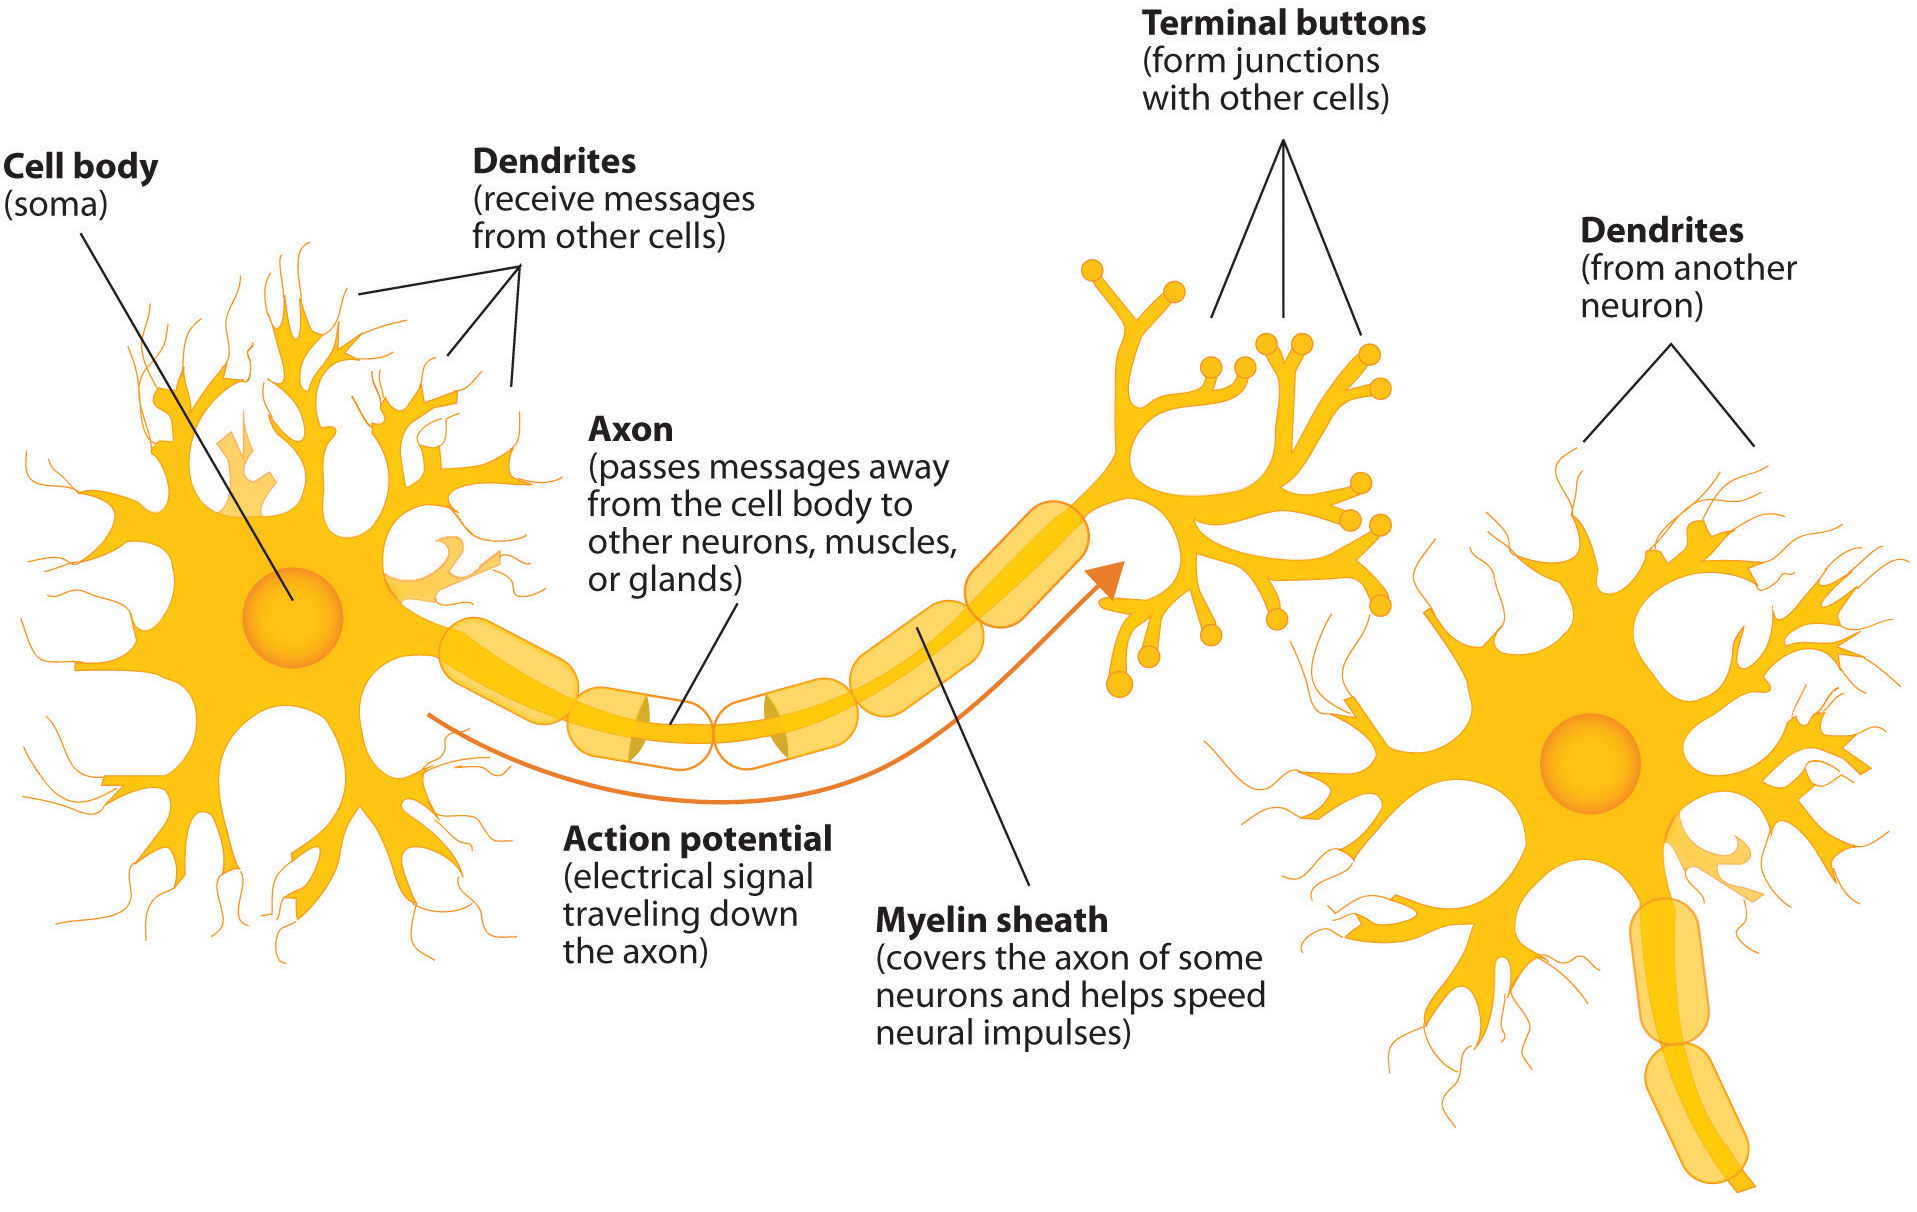
\includegraphics[width=0.99\textwidth]{components_of_neuron}
    \caption[Diagram of the components of a biological neuron]{A Diagram of the components of a biological neuron. The image is from \citeay{wiki_neuron}.}
    \figlbl{components_neuron}
\end{figure}

A biological neuron (c.f. \figref{components_neuron}) is a cell that communicates with other neurons through connections called synapses.
Communication takes place through precisely timed electrical pulses called spikes.
Biological neurons are electrically excitable by voltage changes across their membranes.
If the changes are significant enough within a short interval, the neuron generates a pulse called an action potential.
This action potential travels through the axon and activates synaptic connections.
Other neurons, connected through synapses, receive this signal.
The synaptic signal can be excitatory \sidecite{Takagi_2000} or inhibitory \sidecite{Coombs_Eccles_Fatt_1955}, making the post-synaptic neuron more or less likely to fire an action potential.
Biological neurons can be classified into sensory neurons, motor neurons, and interneurons.
Sensory neurons respond to external stimuli such as light or sound and send signals to the spinal cord or the brain.
Motor neurons receive brain and spinal cord signals to control muscles or organs.
Interneurons connect neurons within the same region of the brain or of the spinal cord.
Multiple connected neurons form a neural circuit.
The neural network in the brain is not static but changes through growth and reorganisation.
This process is referred to as neuroplasticity or neural plasticity \sidecite{Costandi_2016}.

Like a biological neuron, an artificial neuron is connected to other neurons.
Artificial neurons are usually organised in layers that forward signals sequentially.
Although the neurons in the first layer could be considered sensory neurons, the neurons in the last layer could be considered motor neurons, and the neurons in the middle layer could be considered interneurons, such a distinction makes less sense because the artificial neurons function similarly regardless of their layer except for the activation function.
Several variants for artificial neurons have been proposed in the literature. These variants are described in the following  \secref{ann}.
Like biological neurons, multiple artificial neurons are connected to artificial neural networks.


\section{Artificial Neural Networks}\seclbl{ann}
The idea for artificial neural networks (ANN) stems from biology and aims to capture the interaction of biological neurons with a mathematical model.
McCulloch and Pitts proposed the first model for a neuron that can be connected to other neurons in 1943 \sidecite{McCulloch_Pitts_1943}.
Similar to how a neuron of the human brain transmits electrical impulses through the nervous system, the artificial neuron of McCulloch and Pitts receives multiple input signals and transforms them into an output signal.
A neuron takes an input vector $\boldsymbol{x} = (x_1, ..., x_n)$ where $x_i \in \{0, 1\}$ and maps it to an output $\hat{y} \in \{0, 1\}$.
The mapping from the input to the output is done by using an aggregation function $g(\cdot)$ that sums up the input vector $\boldsymbol{x}$ and an activation function $f(\cdot)$ that outputs $1$ if the output of $g(\cdot)$ is bigger than a threshold $\theta$ and $0$ otherwise.
%
\begin{equation}\eqlbl{McCulloch_Pitts_agg}%
	z = g(\boldsymbol{x}) = g(x_1, ..., x_n) = \sum_{i=1}^{n}x_i\\
\end{equation}
%
\begin{equation}\eqlbl{McCulloch_Pitts_act}%
		\hat{y} = f(z) = \begin{cases}
      		1, & \text{if}\ z \geq \theta \\
      		0, & \text{otherwise}
    	\end{cases}
\end{equation}
%
In 1958, \sideciteay{Rosenblatt_1958} developed the Perceptron, which works with real numbers as input.
The input vector $\boldsymbol{x} \in \mathbb{R}^n$ is multiplied with a weight vector $\boldsymbol{w} \in \mathbb{R}^n$ with the same length $n$.
%
\begin{equation}\eqlbl{Perceptron_agg}%
	z = g(\boldsymbol{x}) = g(x_1, ..., x_n) = \sum_{i=1}^{n} w_i \cdot x_i\\
\end{equation}
%
The output $\hat{y} \in \{0, 1\}$ is similar to the McCulloch and Pitts neuron $1$ if the aggregated value is greater than a threshold $\theta$ and $0$ otherwise as described in \eqref{McCulloch_Pitts_act}. With real numbers as input, the equations \eqref*{Perceptron_agg} and \eqref*{McCulloch_Pitts_act} can be rewritten as
%
\begin{equation}\eqlbl{Perceptron}%
		\hat{y} =f(g(\boldsymbol{x})) = \begin{cases}
      		1, & \text{if}\ z - \theta \geq 0 \\
      		0, & \text{otherwise}
    	\end{cases}
\end{equation}
%
Later, the step-function \(f(\cdot)\) was replaced with other functions so that the output can also be a real number \(\hat{y} \in \mathbb{R}\). Often-used activation functions are
%
\begin{equation}\eqlbl{act_functions}%
	\begin{aligned}
		\text{Sigmoid: } & \sigma(z) = \frac{1}{1+\mathrm{e}^{-z}}\\
		\text{Rectified linear unit (ReLU): } & (z)^{+} = \max\{0, z\}\\
		\text{Hyperbolic tangent (tanh): }  & \tanh(z) = \frac{\mathrm{e}^{z}-\mathrm{e}^{-z}}{\mathrm{e}^{z}+\mathrm{e}^{-z}}
	\end{aligned}
\end{equation}
%
By convention, a positive bias $b$ is often used instead of the negative threshold $- \theta$, which leads to:
%
\begin{equation}\eqlbl{nn}%
	z = g(\boldsymbol{x}) = \boldsymbol{w} \cdot \boldsymbol{x} + b = \left( \sum_{i=1}^{n}w_i \cdot x_i \right) + b
\end{equation}
%
The neuron's output is calculated with the activation function of $z$:
%
\begin{equation}\eqlbl{nn2}%
	\hat{y} = f(z)
\end{equation}
%
So far, only the output of a single neuron has been discussed.
However, the brain consists of multiple neurons which are connected through synapses.
Therefore, also ANNs consist not only of one neuron but combine multiple neurons in a network. 
These neurons are organized in layers.
In the simplest case, all neurons from one layer are connected with all neurons of the subsequent layer. This is called a fully connected layer.
For a network with multiple neurons within one layer, the input $\boldsymbol{x}$ is fed into all neurons to obtain $\boldsymbol{\hat{y}}$.
If the layer has $k$ neurons, the output of the aggregation function becomes a vector $\boldsymbol{z} = (z_1, ..., z_k)$. The same applies to the output of the activation function $\boldsymbol{y} = (y_1, ..., y_k)$ and the bias $\boldsymbol{b} = (b_1, ..., b_k)$. The weight vector, on the other hand, becomes a matrix $\boldsymbol{W} = (\boldsymbol{w}_1, ..., \boldsymbol{w}_k)$. For a layer with multiple neurons, \eqref{nn} and \eqref{nn2} can be rewritten with matrix operations:
%
\begin{equation}\eqlbl{nn3}%
	\boldsymbol{z} = \boldsymbol{W} \cdot \boldsymbol{x} + \boldsymbol{b}
\end{equation}
\begin{equation}
	\hat{\boldsymbol{y}} = f(\boldsymbol{z})
\end{equation}
%
which is equal to
%
\begin{equation}\eqlbl{nn4}%
		\boldsymbol{z} = \begin{bmatrix}
			z_1\\
			z_2\\
			...\\
			z_k\\
		\end{bmatrix} = \begin{bmatrix}
			\boldsymbol{w}_1 \cdot \boldsymbol{x} + b_1\\
			\boldsymbol{w}_2 \cdot \boldsymbol{x} + b_2\\
			...\\
			\boldsymbol{w}_k \cdot \boldsymbol{x} + b_k\\
		\end{bmatrix} = \begin{bmatrix}
			\left( \sum_{i=1}^{n}w_{1i} \cdot x_i \right) + b_1\\
			\left( \sum_{i=1}^{n}w_{2i} \cdot x_i \right) + b_2\\
			...\\
			\left( \sum_{i=1}^{n}w_{ki} \cdot x_i \right) + b_k\\
		\end{bmatrix}
\end{equation}
\begin{equation}\eqlbl{nn5}%
		\hat{\boldsymbol{y}} = \begin{bmatrix}
			y_1 = f(z_1)\\
			y_2 = f(z_2)\\
			...\\
			y_k = f(z_k)\\
		\end{bmatrix}
\end{equation}
%

The universal approximation theorem\sidecite{Cybenko_1989} proves that a shallow network with one hidden layer (i.e. one layer between input and output layer) and enough neurons can approximate any mapping function between inputs and outputs.
However, very complex mapping functions may need too many neurons in the hidden layer.
Sequentially arranging multiple layers is much more efficient for approximating complex functions.
A sequential arrangement allows learning a hierarchy of features by dividing the mapping function over several successive processing steps.

In an MLP, the input \(\boldsymbol{x}\) is fed into the first layer, and each subsequent layer \(l\) uses the output of the previous layer \(l-1\) as input.
For a network with \(L\) layers, we denote the layer index as superscript square brackets, i.e. $(\cdot)^{[l]}$.
For example, the weights of layer $l$ are denoted as $\boldsymbol{W}^{[l]}$, the bias as \(\boldsymbol{b}^{[l]}\), the output of the aggregation function as \(\boldsymbol{z}^{[l]}\), and the output of the activation function as \(\boldsymbol{a}^{[l]}\).
The input in the first layer is the input data, i.e. $\boldsymbol{a}^{[0]} = \boldsymbol{x}$, and the output of the last layer is the model's prediction, i.e. $\boldsymbol{a}^{[L]} = \hat{\boldsymbol{y}}$. Thus, the mathematical model of an MLP is defined as

\begin{equation}\eqlbl{mlp}
		\boldsymbol{z}^{[l]} = \boldsymbol{W}^{[l]}\boldsymbol{a}^{[l-1]} + \boldsymbol{b}^{[l]}
\end{equation}
\begin{equation}\eqlbl{mlp2}
		\boldsymbol{a}^{[l]} = f({z}^{[l]})
\end{equation}

So far, only the forward pass used to calculate the output $\boldsymbol{\hat{y}}$ has been discussed.
However, the model output $\boldsymbol{\hat{y}}$ will only be close to the target output $\boldsymbol{y}$ if the weights $\boldsymbol{W}^{[l]}$ and biases $\boldsymbol{b}^{[l]}$ are properly defined in every layer $l$.
These parameters are learned during a training period.
The training can take place in a supervised, semi-supervised, self-supervised (sometimes also called unsupervised), or reinforcement learning setting.
In supervised learning, the output of the model $\boldsymbol{\hat{y}}$ is compared to a given target output $\boldsymbol{y}$.
On the other hand, unsupervised learning tries to find patterns in the input data $\boldsymbol{x}$ and cluster the samples into meaningful groups without using pre-defined target labels. Typically, the target $\boldsymbol{y}$ is derived from the data automatically (e.g. predict a masked part of the data); since the model creates the target by itself, this approach is also called self-supervised.
Semi-supervised learning is a hybrid approach of the aforementioned principles that combines a small amount of labelled data with a large amount of unlabelled data.
Lastly, reinforcement learning algorithms aim to maximize the reward that they receive from an environment based on some action they executed.

These learning principles have in common that a loss function (also called objective function) $\mathcal{L}(\cdot)$ can calculate a loss value based on the model output $\boldsymbol{\hat{y}}$ and the target output ${\hat{y}}$. For example, the mean square error (MSE) can be used for regression problems or the negative log-likelihood for classification problems.
The chosen loss function is minimized iteratively with stochastic gradient descent (SGD)\sidenote{there also exist other optimization algorithms such as SGD with momentum, RMSprop, or Adam \citep{Kingma2015AdamAM}} until the network converges to a (local) minima.
The idea behind stochastic gradient descent is to make use of the fact that the negative gradient of the loss value points to the direction of the steepest descent (i.e. in the direction where the loss becomes smaller).
Therefore, SGD updates the network parameters by taking a step of size $\eta$ toward their negative gradient:
%
\begin{equation}\eqlbl{sgd}
	\begin{aligned}
		\Delta \boldsymbol{W}^{[l]} = & -\eta \cdot \left( \nabla_{\boldsymbol{W}^{[l]}} \mathcal{L} \right)\\
		\boldsymbol{W}^{[l]} \coloneqq & \boldsymbol{W}^{[l]} + \Delta \boldsymbol{W}^{[l]}
	\end{aligned}
\end{equation}
%
and
%	
\begin{equation}\eqlbl{sgd2}	
	\begin{aligned}
		\Delta \boldsymbol{b}^{[l]} = & -\eta \cdot \left( \nabla_{\boldsymbol{b}^{[l]}} \mathcal{L} \right)\\
		\boldsymbol{b}^{[l]} \coloneqq & \boldsymbol{b}^{[l]} + \Delta \boldsymbol{b}^{[l]}
	\end{aligned}
\end{equation}
%
The term $\left( \nabla_{\boldsymbol{W}^{[l]}} \mathcal{L} \right)$ is the gradient of the weights \(\boldsymbol{W}^{[l]}\)  with respect to the loss $\mathcal{L}(\cdot)$ and the term $\left( \nabla_{\boldsymbol{b}^{[l]}} \mathcal{L} \right)$ is the gradient of the bias \(\boldsymbol{b}^{[l]}\)  with respect to $\mathcal{L}(\cdot)$.
The gradients of the weights can efficiently be calculated with an algorithm called backpropagation of error \sidecite{Rumelhart_Hinton_Williams_1986}, which is, in fact, just an intelligent implementation of the chain rule\sidenote{While a detailed discussion on backpropagation is out of scope for this thesis, we refer interested readers to the deep learning course by Andrew Ng \cite{Coursera}}.

One of the most critical design decisions in creating ANNs is how the neurons are connected.
So far, only the case where every neuron of one layer is connected to every neuron of the following layer (so-called fully connected layer) has been described. 
Besides such dense connections, there are several alternatives.
Since this work deals with the processing of visual scenes, the most well-known image-processing network architecture, namely Convolutional Neuronal Networks (CNN), is presented below. This architecture is also primarily used in this thesis. However, various alternative architectures exist for computer vision, such as Vision Transformer (ViT) \sidecite{Dosovitskiy_Beyer_Kolesnikov_Weissenborn_Zhai_Unterthiner_Dehghani_Minderer_Heigold_Gelly_2021} or MLP Mixer \sidecite{tolstikhin2021mlp}, which, however, would go beyond the scope of this introduction to deep learning.























\subsection{Convolutional Networks}\seclbl{cnns}
Convolutional Neural Networks (CNNs) are particularly useful for finding patterns in images but can also be used to analyze non-image data such as audio data or time series.
Similar to FCNs, a CNN is composed of an input layer, an output layer, and many hidden layers in between.
A typical CNN consists of subsequently connected convolutional layers and pooling layers.
Usually, an activation function is applied after each convolutional layer while no activation function is used after pooling layers.
Depending on the task, the last layers can be different, e.g. for image classification the last layers are often fully connected.

Convolutional layers use convolution filters or kernels that slide along input features and create translation-equivariant\sidenote{most CNNs apply downsampling operations to the input and are therefore not translation-invariant but translation-equivariant \cite{Mouton_Myburgh_Davel_2020}} responses known as feature maps \sidecite{Zhang_Itoh_Tanida_Ichioka_1990}.
The size of the filter, which is typically a \(3\times 3\) matrix, determines the size of the receptive field.
The filter is applied to an area of the input, with that area having the same size as the filter.
When applying the filter, the dot product is calculated between the input and the filter and then fed into an output array (i.e. the feature map).
Afterwards, the filter shifts by a stride, repeating the process until the entire input has been processed.
Since only the kernel have to be learned, convolutional layers consists of much less parameters than equivalently sized fully connected layers.
This process of re-using the same weights at different locations of the input is also known as parameter sharing.
As described earlier, multiple convolutional layer can follow on each other.
By doing so, CNNs become hierarchical as the later layers can see the pixels within the receptive fields of prior layers.

Pooling layers reduce the size of the input by conducting dimensionality reduction.
Similar to convolutional layers, a filter slides along the input.
However, this filter does not have any learned parameter but apply an aggregation function.
Usually, the filter either select the pixel with the highest value (max pooling) or calculates the average (average pooling) within the receptive field and forwards it to the output array.
Pooling layers usually discard a lot of information but help to reduce complexity and increase robustness.

In the last decades, various CNN architectures have been proposed, usually consisting of different combinations of CNN and pooling layer.
Further improvements have been achieved by using parallel paths of convolutional layers, batch normalization \sidecite{Ioffe_Szegedy_2015}, and skip connections\sidenote{skip connections skips some of the layers in the network and add the output of a layer to the input of a later layer}.
In this thesis I do not go into these specific architectures but provide some references to some well known architectures; LeNet \sidecite{Lecun_Bottou_Bengio_Haffner_1998}, AlexNet \sidecite{NIPS2012_c399862d}, VGGNet \sidecite{Simonyan_Zisserman_2015}, GoogLeNet \sidecite{Szegedy_Liu_Jia_Sermanet_Reed_Anguelov_Erhan_Vanhoucke_Rabinovich_2014}, ResNet \sidecite{He_Zhang_Ren_Sun_2016}, U-Net \sidecite{Ronneberger_Fischer_Brox_2015}, Mask R-CNN \sidecite{He_Gkioxari_Dollar_Girshick_2017}, SSD \sidecite{Liu_Anguelov_Erhan_Szegedy_Reed_Fu_Berg_2016}, and YOLO \sidecite{Redmon_Divvala_Girshick_Farhadi_2016}.

\subsubsection{Training of Convolutional Neural Networks}\seclbl{train_cnns}
CNNs can be used in various applications such as image recognition, video analysis, natural language processing, anomaly detection in time series and many others.
Since this thesis deals with better representations for visual scenes, this chapter is limited to the typical image analysis tasks; image classification, object detection, and image segmentation.
An overview of these tasks is shown in Figure \figref*{img_analysis_tasks}.
The goal of image classification is to predict an image-level label, i.e. to predict what object is in the image.
A classic example of this problem is predicting whether a cat or a dog is in a picture.
This is typically done for images that only contain one object.
With a multi-label classifier, however, it is also possible to predict whether none, one or several classes are present, i.e. whether a cat, a dog or both are present in the image.
With image classification it is unclear where in the image these objects are located.
Object detection provides a remedy.
The aim of object detection is not only to determine what is visible in the image but also where.
The position of the object is usually indicated by a bounding box (i.e. a rectangle).
Especially when there are several objects within a picture, it is helpful to know which object is where, e.g. that the cat is to the left of the dog.
For some applications, predicting the position with bounding boxes is not sufficient.
In this case, semantic segmentation is often used.
Semantic segmentation is the task where each pixel is classified (the image is divided into segments) which leads to a pixel-wise mask for each object in the image.
This gives us exact information about the shapes of the objects.

\begin{figure}[h]
    \centering
    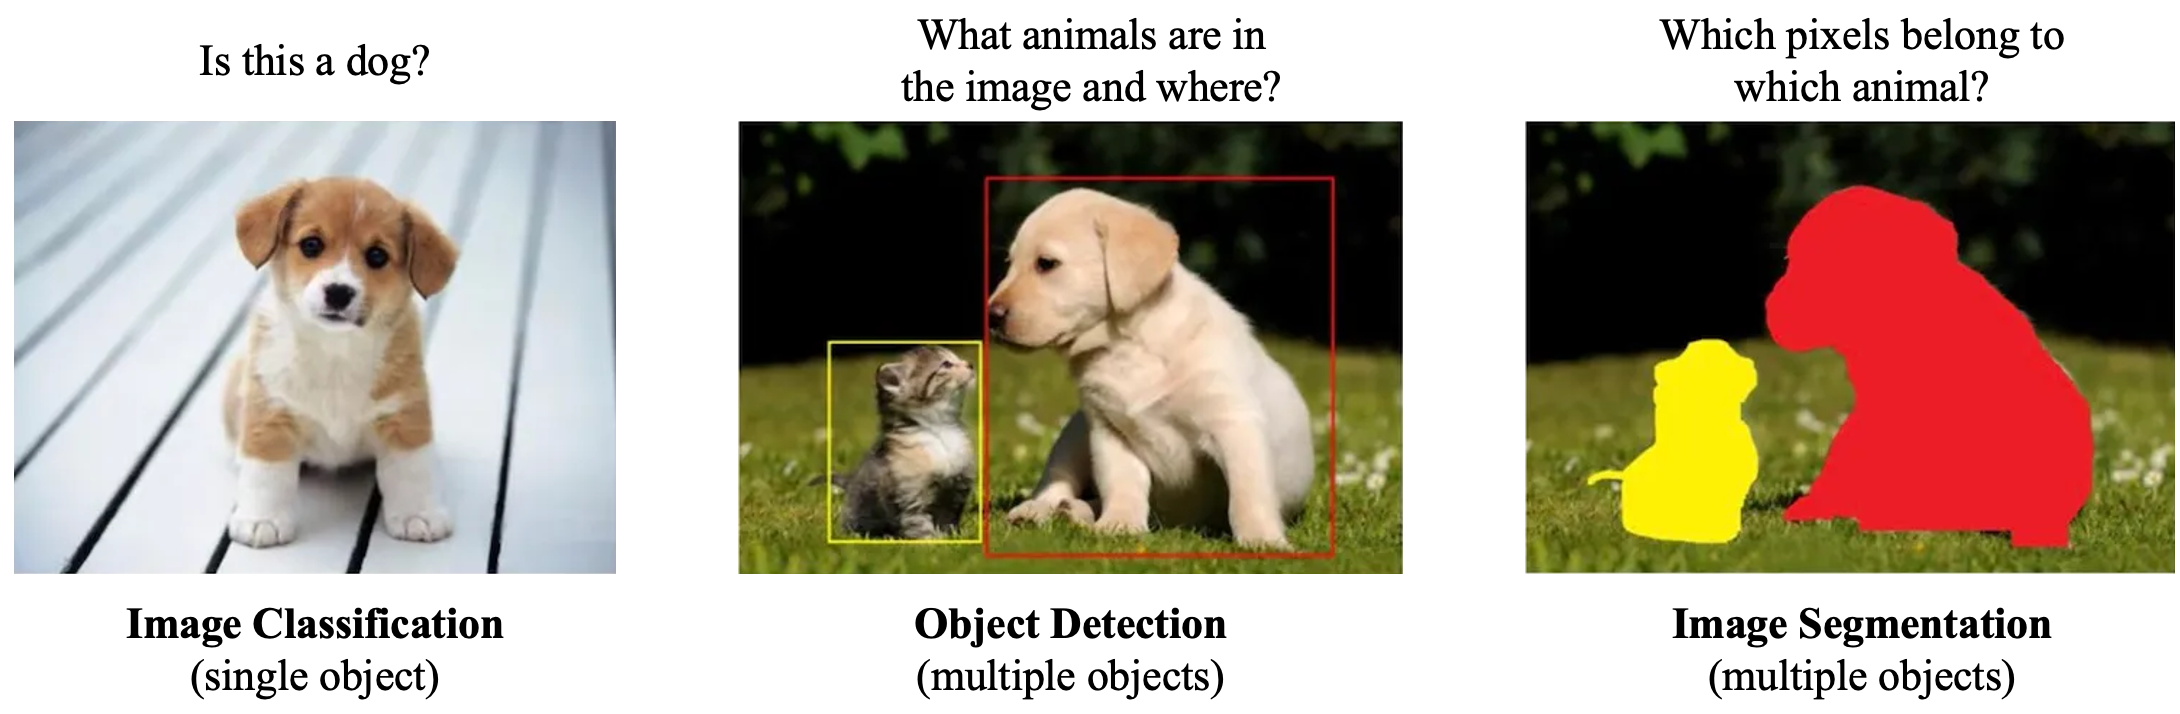
\includegraphics[width=0.99\textwidth]{image_analysis}
    \caption[Overview of different image analysis tasks]{Overview of different image analysis tasks. The image is taken from \citeay{venturebeat_img_analysis} and was slightly adapted.}
    \figlbl{img_analysis_tasks}
\end{figure}


Depending on the task, different kind of labels are required for supervised learning.
Image classification requires labels on image-level (i.e. one or multiple labels per image) \cite{Lecun_Bottou_Bengio_Haffner_1998, NIPS2012_c399862d, Simonyan_Zisserman_2015, Szegedy_Liu_Jia_Sermanet_Reed_Anguelov_Erhan_Vanhoucke_Rabinovich_2014, He_Zhang_Ren_Sun_2016}, object detection requires the coordinates of the bounding box \cite{Redmon_Divvala_Girshick_Farhadi_2016, Liu_Anguelov_Erhan_Szegedy_Reed_Fu_Berg_2016, He_Gkioxari_Dollar_Girshick_2017}, and semantic segmentation requires the labels on pixel-level \cite{Ronneberger_Fischer_Brox_2015, Wu_Zhang_Huang_Liang_Yu_2019} (i.e. each pixel has a label of an object or a label ``background'' for irrelevant pixels).

Besides supervised learning, there are various principles of learning with partial labels or without labels.
These techniques are called weakly-supervised or un-supervised learning and are well summarised in \sidecite{Simmler_Sager_Andermatt_Chavarriaga_Schilling_Rosenthal_Stadelmann_2021}.
Not only specific tasks can be learned, but also task-independent representations.
These representations are typically learned unsupervised\sidenote{also called self-supervised learning because the target labels are derived from the data itself} and can be used for one or several downstream tasks.
More details on visual representation learning are provided in Section \secref*{visual_rep_learning}.
Especially Autoencoders \sidecite{rumelhart1985learning} are explained in this section as they are applied in this thesis.


\section{Limitations}\seclbl{limitationsDL}
The rise of deep learning over the past decade has only been possible because of major technological advances in hardware.
Without the computational resources and the storage capacity of the systems created in the last decades no system could run today's algorithm.
Moreover, much of the progress of recent years was possible due to the improved hardware. 
Moore’s law \cite{Moore_2006} states that the number of transistors in a dense integrated circuit doubles about every two years and is the only known physical process following an exponential curve.
An analysis by OpenAI shows that since 2012 the amount of compute has even increasing exponentially with a doubling time  of \(3.4\) months \cite{OpenAI_compute}.
However, the exponential increase seems to come to an end since the size of transistors hit physical limitations.
It is assumed that Moore's law will end by around 2025 \sidecite{Kumar_2015}.
Besides the progress in the field and the development of new technology, deep learning models also became better because the number of parameters and the size of datasets grew exponentially.
Even the growth in the last five years is astonishing.
While the state-of-the-art language model from 2018 \sidecite{Peters_Neumann_Iyyer_Gardner_Clark_Lee_Zettlemoyer_2018} had around \(94\)M parameters, the state-of-the-art in 2020 \sidecite{NEURIPS2020_1457c0d6} already had \(175\)B parameters. Training such a model on a single V100 GPU would take about 355 years and cost about \(4.6\)M dollars \cite{Lambda_GPT3}.
A recent language model from Microsoft and Nvidia \sidecite{Shoeybi_Patwary_Puri_LeGresley_Casper_Catanzaro_2020} even has \(530\)B parameters.
Only a few institutions with massive resources are able to train such big models.
In general, inference on low-budget hardware such as smartphones or embedded hardware becomes prohibitive with the growing size of deep networks.
Even tough there exist techniques to shrink the model size after training such as quantization \cite{Wu_Judd_Zhang_Isaev_Micikevicius_2020}, model pruning \cite{Choudhary_Mishra_Goswami_Sarangapani_2020}, or model distillation \cite{Hinton_Vinyals_Dean_2015} it is questionable if making models bigger is the best way to develop intelligent systems.

Another major issue of deep learning systems is that they suffer from catastrophic forgetting.
If a model is trained on a specific task and afterwards trained (or fine-tuned) on another task, the model suffers a ``catastrophic'' drop in performance over the first task.
The reason for this effect is that the model during training on the second task adjusts the parameters learned during the first task and therefore ``forgets'' the learned mapping functions.
Just mixing all datasets or to learn all tasks in parallel in a current multi-task setup \cite{Zhang_Yang_2021} doesn't seem feasible to achieve some kind of general intelligence as this involves too many different unrelated tasks.
Catastrophic forgetting is also caused by the fact that learning is mostly done offline\sidenote{Offline in this context means that the model parameters are not adapted after training during inference time}.
Online learning \cite{Sahoo_Pham_Lu_Hoi_2017} and lifelong learning \cite{Parisi_Kemker_Part_Kanan_Wermter_2019} are currently hot research topics.
However, these methods have not yet been established.

Furthermore, there exists problems which may cannot be solved with the current principles used for deep learning.
First of all, it is questionable if deep learning models can achieve \emph{real} generalization\sidenote{Generalization refers to the ability of the model to adapt properly to previously unseen data from the same distribution}.
With enough data, can achieve generalization in the sense that the model can interpolate within the data distribution.
However, deep learning models fail to extrapolate.
For example, convolutional neural networks (CNNs) do not generalize to different viewpoints unless they are added to the training data \sidecite{Madan_Henry_Dozier_Ho_Bhandari_Sasaki_Durand_Pfister_Boix_2022}.

Second, deep learning is not able to learn abstract relationships in a few trials but requires many samples of it and is thus data hungry.\sidenote{Delme!!!}
Marcus Gary \sidecite{Marcus_2018} argues that if he tells that a ``schmister'' is a sister over the age of 10 but under the age of 21, humans can  immediately infer whether they or their best friends have any ``schmister''. However, modern DL systems lacks a mechanism for learning abstractions through explicit, verbal definition and require thousands or even more training samples.

Third, no DL model has been able to demonstrate causal reasoning in a generic way.
Deep learning models find correlations between the inputs and the outputs, but not the causation.
Other AI approaches such as hierarchical Bayesian computing or probabilistic graphical models are better at causal reasoning but cannot be well combined with deep learning models.

Lastly, deep learning models are to some extend too isolated since they have no embodiment and cannot interact with the world.
For example, the human body provides needs, goals, emotions, and gut feeling\sidenote{one could argue that the body is therefore even a co-processor of the brain}.
In current deep learning systems are emotions totally absent and the goals are set externally.
Deep Reinforcement Learning can be considered as a first step in the direction of dissolving this isolation, as they interact with a virtual environment. 
AI systems that interact with the real world do not work well so far.
Moravec's paradox \sidecite{Moravec_1995} states that ``it is comparatively easy to make computers exhibit adult level performance on intelligence tests or playing checkers, and difficult or impossible to give them the skills of a one-year-old when it comes to perception and mobility''.


\section{Biological Learning}\seclbl{biological_learning}
The human brain comprises many interconnected areas processing everything in parallel.
For example, Figure \figref{visual_cortext} illustrates the connections between different organizational units in the cerebral cortex which are responsible for vision.
It can be seen that these areas are connected in a rather complex structure.
\begin{figure}[h]
    \centering
    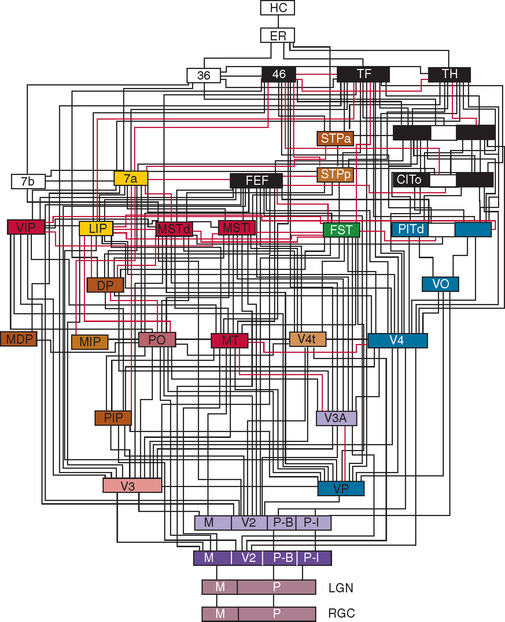
\includegraphics[width=0.99\textwidth]{felleman_visual_cortex}
    \caption[Organization of the visual system in the cerebral cortex]{The organization of the visual system in the cerebral cortex. The image is from \citeay{Felleman_Van_Essen_1991}.}
    \figlbl{visual_cortext}
\end{figure}
Deep learning architectures, on the other hand, are mostly unidirectional and the signal flows unidirectional from layer to layer\sidenote{Except for recurrent connections, skip-connections, or residual-connections}.
However, the choice of the architecture influences the how the model can learn the mapping function from input to output.
It could be that the complex structure of our brain comprises an inductive bias which was learned over time through evolution.

A learning system requires a mechanism that tells the system if something goes well or wrong so that it can learn from it.
This is called the \emph{credit assignment problem}.
Backpropagation (c.f. Section \secref*{fundamentalsDL}) solves this problem by propagating the error backwards through the network.
However, information flows in the brain only in one direction from the presynaptic neurons to the postsynaptic neurons.
Therefore, backpropagation is not biologically plausible.
Lillicrap et al. \sidecite{Lillicrap_Cownden_Tweed_Akerman_2016} shows that an additional set of random feedback weights is able to transmit useful gradients.
Their work has reopend questions how the brain could process error signals and has dispel some long-held assumptions about algorithmic constraints on learning.

Not only the structure of the network and the way how the feedback is calculated is different between biological learning and deep learning.
Also the neurons themselves are different.
While the artificial neuron doesn't have any dynamics (c.f. Equation \eqref*{nn}), biological neurons are highly dynamic:
Biological neurons adapt their firing rate to constant inputs, they may continue firing after an input disappears, and can even fire when no input is active (c.f. Section \secref*{reservoir_comp}).

Lastly, the neurons in the brain are self-organizing.
This means that a group of elementary units such as neurons or a group of neurons perform similar rule of behavior on a sub-set of the available information.
Such a system doesn't have a central supervision that orchestrates these units.
Each unit applies similar deterministic functions to the information received.
Two important principles of such systems are (i) localized learning which means that each unit adapt their behavior to the information they receive; and (ii) emergence which means that there is no explicit loss function that tells the system what to do.


\section{Neurocomputing}\seclbl{neurocomputing}

\subsection{Hebbian Learning}\seclbl{hebbian}
Donald Hebb \sidecite{Hebb_1949} describes how the connections between cells in the nervous system adapt as: ``When an axon of cell A is near enough to excite a cell B and repeatedly or persistently takes part in firing it, some growth process or metabolic change takes place in one or both cells such that A’s efficiency, as one of the cells firing B, is increased''. This statement is often simplified to the well-known phrase ``Neurons that fire together wire together''.

Hebbian learning is based on this principle.
The weight \(w_{ij}\) from neuron \(i\) to neuron \(j\) changes based on the pre-synaptic activity \(r_i\) of neuron \(i\) and post-synaptic activity \(r_j\) of neuron \(j\)

\begin{equation}\eqlbl{hebb_1}
	\Delta w_{ij} = \eta r_i r_j
\end{equation}

where \(\eta\) is the learning rate.
Thus, the weights between frequently co-activated neurons becomes strong which is called Hebbian plasticity.

In its original form, Hebbian learning had the problem that the connections could only become stronger but not weaker.
Therefore, it is often extended based on the covariance of the activity between neurons.
The covariance is positive if two neurons fire often together and negative if they do not often fire together.
The following equation changes the weight relative to the covariance:

\begin{equation}\eqlbl{hebb_2}
	\Delta w_{ij} = \eta (r_i - \psi_i) \cdot (r_j - \psi_j)
\end{equation}

where \(\psi_i\) and \(\psi_j\) are estimates of the expected pre- and post-synaptic activity\sidenote{the expected activity can for example be estimated through a moving average function}.
The formulation above lacks of boundaries, i.e. the weights could grow to infinite.
A simple solution is to enforce hard boundaries \(w_{min} \leq w_{ij} \leq w_{max}\).

Another solution to weaken the connections is given by the Bienenstock-Cooper-Monroe (BCM) learning rule which was introduced by Bienenstock et al. \sidecite{Bienenstock_Cooper_Munro_1982} and extended by Intrator and Cooper \sidecite{Intrator_Cooper_1992}.
They propose a sliding threshold for long-term potentiation (LTP) or long-term depression (LTD) induction.
When a pre-synaptic neuron fires and the post-synaptic neuron is in a lower activity state than the sliding threshold, it tends to undergo a LTD (i.e. the connection is weaken).

Around the same time, Oja \sidecite{Oja_1982} improved the learning rule of Equation \eqref*{hebb_1} with an normalization term:

\begin{equation}\eqlbl{hebb_3}
	\Delta w_{ij} = \eta (r_i r_j - \alpha r^2_j w_{ij})
\end{equation}

The parameter \(\alpha\) is a constant value that determines the size of the norm of the weight vector.
This update rule is also known as the Oja learning rule. 
Furthermore, he has found that a layer of multiple linear neurons converges to the first principle component of the input data.
As all neurons only learn the first principle component, a network of multiple neurons in this setting seem not very useful.
Differentiation between neurons can be achieved with several different methods.
Two well known approaches are the winner-take-all competition (i.e. only the neuron with the most similar activity is selected for learning)\sidenote{in practice is k-winner-take-all often preferred where k instead of one neuron learns} and a recurrent circuit that provides a competitive signal (i.e. the neurons compete with their neighbours to become active to learn).

It is known that independent neurons can encode more information and work better than dependent neurons \sidecite{Simoncelli_Olshausen_2001}.
Anti-Hebbian learning is a method that adds a penalty for similarly active neurons and thus minimizes the linear dependency between neurons.
Vogels et al. implemented this by switching the sign of the weight change \sidecite{Vogels_Sprekeler_Zenke_Clopath_Gerstner_2011}.

There exists many further improvements for Hebbian learning which are not summarized in this thesis.
For example, Joshi and Triesch \sidecite{5178625} as well as Teichmann and Hamker \sidecite{Teichmann} adapt the activation function of the neurons to enforce a certain activity distribution and to stabilize Hebbian learning even in multilayer neural networks.

Similar to large parts of the brain, Hebbian learning is unsupervised and learns based on local information (i.e. neurons in close proximity).
However, the brain is also largely recurrent and could guide neighbouring or preceding units.
This assumption inspired supervised Hebbian learning.
In supervised Hebbian learning, a subset of inputs which should evoke post-synaptic activity can be selected.
Supervised Hebbian learning can be extended to top-down and bottom-up learning \sidecite{Grossberg_1988} which leads to a combination of supervised and unsupervised Hebbian learning.


\subsection{Hopfield Networks}\seclbl{hopfield}
Hopfield networks \sidecite{Hopfield_1982} were introduced 1982 by J. Hopfield.
They serve as associative (i.e. content-adressable) memory systems.
Such systems are particularly useful to retrieve representations based on degraded or partial inputs.
Auto-associative memories return for an input the most similar previously seen sample.
A classical implementation of an auto-associative memory is the nearest neighbour algorithm \sidecite{Fix_Hodges_1989}.
This algorithm compares a given samples with the previously seen training data with a distance metric and returns the most similar sample\sidenote{or the \(k\) most similar samples in the case of the k nearest neighbour (k-NN) algorithm}.
Memory networks \sidecite{Weston_Chopra_Bordes_2015} implement an auto-associative memory within the deep learning framework.
Such networks convert an input \(\boldsymbol{x}\) to a internal feature representation \(I(\boldsymbol{x})\), update memories given the new input \(m=G(m, I(\boldsymbol{x}))\), and compute the output features \(o=O(m, I(\boldsymbol{x}))\).
This process is applied during the training and inference phase.
The only difference is that the parameters for the functions \(I\), \(G\), and \(O\) are only updated during training.

In a Hopfield network are all neurons are connected, but there are no self-connections: \(w_{ii}=0\) where \(w_{ij}\) is the weight between neuron \(i\) and neuron \(j\).
Furthermore, the weights are symmetrical \(w_{ij} = w_{ji}\).
A Hopfield network in its original form works only with binary units.
For consistency, this networks are called binary Hopfield networks in the following.
The output of a neuron in a binary Hopfield network depends on the output of the other neurons within the network:

\begin{equation}\eqlbl{hf_1}
	x_i = \sum_{i \neq j} w_{ij} y_j + b
\end{equation}

\begin{equation}\eqlbl{hf_2}
	y_i = \begin{cases}
      		1, & \text{if} x > 0 \\
      		-1, & \text{otherwise}
    	\end{cases}
\end{equation}

TODO in equation: check where to use y and where to use y with hat


Hopfield networks have their own dynamics and the output evolves over time.
If the initial value \(y_i\) of a binary Hopfield network has a different sign than \(\sum_{i \neq j} w_{ij}y_j + b\) the output will flip (i.e. change its sign).
This will in turn influence all other neurons which may also flip.
The term \(y_i(\sum_{i \neq j} w_{ij}y_j + b)\) is negative if \(y_i\) is not equal to \(\sum_{i \neq j} w_{ij}y_j + b\), otherwise it is positive.
Since the neuron flips if the term \(y_i(\sum_{i \neq j} w_{ij}y_j + b)\) is negative or stays the same if this term is positive, the change of this term can only be positive:

\begin{equation}\eqlbl{hf_3}
	\Delta [y_i(\sum_{i \neq j} w_{ij} y_j + b)] \geq 0
\end{equation}

The negative sum of the term \(y_i(\sum_{i \neq j} w_{ij}y_j + b)\) for the entire network is called the energy \(E\) of the network:

\begin{equation}\eqlbl{hf_4}
	E(\boldsymbol{y}) = -\sum_{i} y_i \left( \sum_{j>i} w_{ji} y_j + b \right)
\end{equation}

As we have shown in \eqref*{hf_3}, the energy function \(E\boldsymbol{y})\) of the network can only decrease.
Moreover, the energy function has a lower bound and thus the network reaches after a finite number of iterations a stable state. 
A stable pattern of the network (i.e. no neurons flip their sign) is a local minima of the energy function and is called a point attractor.
A pattern is attracted by the closest stable pattern.
Thus, the network can be used as associative memory because an input pattern can be matched to the closest stable pattern.

McElice \sidecite{1057328} has shown that a binary Hopfield network with \(N\) neurons has a capacity of \(C=0.138N\) (i.e. the number of patterns that can be stored.
Hebbian learning (c.f. Section \secref*{hebbian}) can be used to store pattern in a Hopfield network.
To store a pattern, the weights \(\boldsymbol{w}\) must be choosen in a way so that the desired local patterns \((\boldsymbol{y}^1, ..., \boldsymbol{y}^P)\) are local minima of the energy function.
By combining Hebbian learning with some smart mathematical transformations it can be shown that the weights can be directly learned with only one iteration over the training patterns\sidenote{for the derivation of this equation refer to \citep{Hopfield_1982}}:

\begin{equation}\eqlbl{hf_5}
	\boldsymbol{w} = \frac{1}{p} \sum_{k=1}^{P} \boldsymbol{y}^k \times (\boldsymbol{y}^k)^T - \boldsymbol{I}
\end{equation}

where \(\boldsymbol{I}\) is the identity matrix.
Later, Hopfield et al. \sidecite{Hopfield1983} extended the binary Hopfield network so that it can either learn pattern during an awake cycle or forget patterns during a sleep cycle.

One of the limiting factors of binary Hopfield networks is the capacity of \(C=0.138N\).
The problems comes from the fact that the energy function is a quadratic function.
More than three decades after the introduction of the binary Hopfield networks, Krotov and Hopfield \sidecite{10.5555/3157096.3157228} reformulated the energy function as a polynomial function to get polynomial capacity \(C\approx N^{a-1}\) where \(a\) is the order of the function.
Later, the energy function was reformulated as exponential function \sidecite{Demircigil_Heusel_Löwe_Upgang_Vermet_2017} and thus modern Hopfield networks have an exponential capacity of \(C\approx 2^{\frac{N}{2}}\).

The second limiting factor of binary Hopfield networks is that only binary patterns can be stored.
Ramsauer et al. \sidecite{Ramsauer} extended the binary Hopfield network to continous patterns by reformulating the energy function and the corresponding update rule.
Continous Hopfield networks can retrieve continous patterns or even combination of several similar continous patterns.
The authors claim that a continous Hopfield networks can replace fully-connected layers, attention layers \cite{10.5555/2969033.2969073}, LSTM layers \cite{Hochreiter_Schmidhuber_1997}, support vector machines (SVM) \cite{Cortes_Vapnik_1995}, and k nearest neighbor (k-NN) \cite{Cover_Hart_1967}.


\subsection{Spiking Neural Networks}\seclbl{spiking_networks}
Biological neurons emit spikes.
To transmit information, especially the firing rate (i.e. the number of spikes per second in Hz) and precise timing of the spikes are relevant.
The amplitude and duration of the spike does not matter much.
This behaviour has also been implemented in ANNs.
So called Spiking neural networks (SNNs) incorporate the concept of time into their model.
SNN do not transmit information in each forward-pass but rather transmit a signal when the membrane potential reaches a threshold value\sidenote{the membrane potential is related to the electrical charge of the membrane of a biological neuron}. 
The neuron fires as soon as the threshold is reached and thereby influences the potential of other neurons.
The most prominent model of a spiking neuron is the leaky integrate-and-fire (LIF) neuron \sidecite{Abbott1999LapicquesIO}.
The LIF neuron models the membrane potential with a differential equation.
Incoming spikes can either increase or decrease the membrane potential.
The membrane potential either decays over time or is reset to a lower value if the threshold value is reached and the neuron has fired.
There exists different integrate-and-fire (IF) neurons models such as the Izhikevich quadratic IF \sidecite{Izhikevich_2003} or the adaptive exponential IF \sidecite{Brette_Gerstner_2005}.
While each of these model gas different mathematical properties, the concept of a membrane potential that is increased or decreased through spikes from other neurons and decays over time or by emitting a spike is similar to the LIF.

Biological neurons have different dynamics.
Some neurons fire regularly if the receive an input current, others slow down the firing rate over time or emits bursts of spikes.
Modern models of spiking neurons can recreate this behaviour of biological neurons \sidecite{Paugam_Moisy}.

The synaptic plasticity can be modeled with Hebbian learning (c.f. Section \secref*{hebbian}).
The spike-timing dependent (STDP) plasticity rule \sidecite{Bi_Poo_2001} distinguishes the tiring behaviour of pre-synaptic and post-synaptic neurons.
If the pre-synaptic neurons fires before the post-synaptic neuron, the connection is strengthen, otherwise it is weaken.

For a long time, SNN only worked for very shallow networks.
In 2018, Kheradpisheh et al. \sidecite{KHERADPISHEH201856} has proposed a SNN based on the idea of CNNs called a deep spiking convolutional network.
This network uses convolutional and pooling layers with IF neurons instead of classical artificial neurones and is trained with STDP.
First, the image is fed into DoG cells.
This cells apply the difference of Gaussians (DoG) feature enhancement algorithm.
This algorithm subtracts a Gaussian blurred version of an image from the original image.
By doing so, positive or negative contrast is detected in the input image.
The higher the contrast is, the stronger is a cell activated and the earlier it emits a spike.
Thus, the order of the spikes depends on the order of the contrast.
These spikes are forwarded to a convolutional layer.
Deep spiking convolutional networks use two types of LIF neurons: On-center neurons fire when a bright area is surrounded by a darker area, off-center neurons do the opposite.
Convolutional neurons emit a spike as soon as they detect their preferred visual feature\sidenote{the location of the feature is not relevant as convolution layers are translation invariant}.
Neurons that fire early perform the STDP update with a winner-takes-all mechanism.
This means that the neurons within a layer compete with each other and those which fire earlier learn the input pattern.
This prevents other neurons from firing and guarantees a sparse connection.
Later convolutional layers detect more complex features by integrating input spikes from the previous layer.
The features from the last convolutional layer are flatten and a Support Vector Machine is used to classify the features.


\subsection{Reservoir Computing}\seclbl{reservoir_comp}
As described in Section \secref*{biological_learning}, biological neurons are highly dynamical while artificial neurons are not.
Reservoir computing introduces such dynamics into an artificial network.
Reservoir computing is an umbrella term for networks based on the concepts of Echo State Networks (ESN) \sidecite{esn} and Liquid State Machines (LSM) \sidecite{Maass_Natschlager_Markram_2002}.
A reservoir is a fixed non-linear system that maps a input vector \(\boldsymbol{x}\) to a higher dimensional computation space.
After the input vector is mapped into computation space, a simple readout mechanism is trained to return the desired output based on the reservoir state.
In principle, the system should be capable of any computation if it has a high enough complexity \sidecite{Konkoli_2018}.
However, not every system is suited as reservoir.
A good reservoir system distributes different inputs into different regions of the computation space \cite{Konkoli_2018}.

A ESN is a set of sparsely connected recurrent neurons as visualized in Figure \figref*{reservoir}.

\begin{figure}[h]
    \centering
    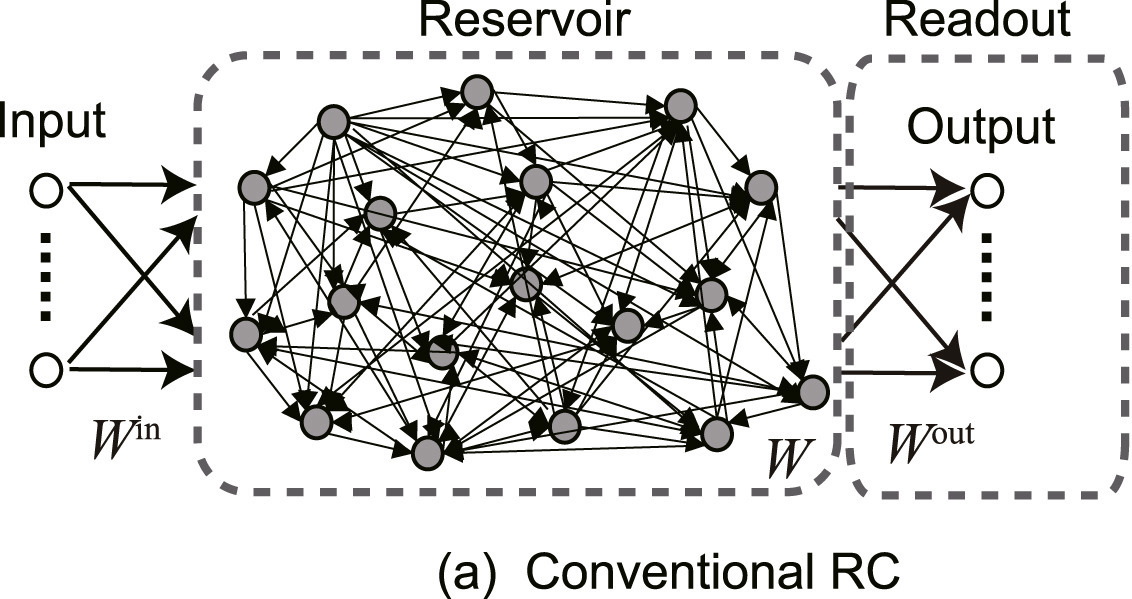
\includegraphics[width=0.99\textwidth]{reservoir}
    \caption[Structure of a Echo State Network]{Structure of a Echo State Network. The image is from \citeay{Tanaka_Yamane_Héroux_Nakane_Kanazawa_Takeda_Numata_Nakano_Hirose_2019}.}
    \figlbl{reservoir}
\end{figure}

The reservoir consists of \(N\) nodes which are connected according a Erdős–Rényi graph model\sidenote{The Erdős–Rényi model is a model for generating random graphs where all graphs on a fixed set of vertices and edges is equally likely} \sidecite{erdos59a}.
This graph model is represented by an adjacency matrix \(\boldsymbol{w}\)\sidenote{Figure \figref*{reservoir} uses upper case letter \(\boldsymbol{W}\)} of size \(N \times N\).
The time varying input signal \(\boldsymbol{x(t)}\) is mapped to a sub-set of \(N/M\) graph nodes by multiplying it with \(\boldsymbol{w}_{\text{in}} \in \mathbb{R}^{N\times M}\) and the output by multiplying the reservoir state with \(\boldsymbol{w}_{\text{out}} \in \mathbb{R}^{M\times N}\).
We refer interested reads to \sidecite{Lukoševičius_2012} to read more about the mathematical properties and how network is updated in detail.

In the original form of ESN, only the readout weights are learned, the rest is chosen randomly.
The input \(\boldsymbol{x(t)}\) brings the recurrent units in a initial state.
The recurrent connections inside the reservoir create different dynamics in the network.
The readout neurons linearly transform the recurrent dynamics into temporal outputs.
The readout weights \(\boldsymbol{w}_{\text{out}}\) are trained to reproduce a target function \(\boldsymbol{y(t)}\).

Liquid State machines use a spiking neural network instead of a graph of recurrent units as reservoir.
The nodes of the spiking neural network are randomly connected together.
Thus, every node receives time varying inputs from the inputs as well as from other nodes.
The recurrent connections turns the varying input into a spatio-temporal pattern.
Similar to ESN, the spatio-temporal patterns of activation are read out by a linear layer.

In general, reservoirs are universal approximators and can approximate any non-linear function given there are enough neurons in the reservoir.
They generalize better and faster than equivalent MLP.
The main drawback of current systems is that cannot deal well with high-dimensional inputs such as images.







\setchapterpreamble[u]{\margintoc}
\chapter{Related Work}\chlbl{rel_work}
%% related_work.tex

\section{Natural Intelligence}\seclbl{natural_intelligence}
This thesis is inspired by the work ''A Theory of Natural Intelligence` from von der Malsburg et al. \sidecite{von_der_Malsburg_Stadelmann_Grewe_2022}.
Therefore, we dedicate this section to summarize their work in detail.

According \cite{von_der_Malsburg_Stadelmann_Grewe_2022}, the process of learning is influenced by ``nature'', ``nurture'', and ``emergence''\sidenote{nature refers to the influence of genes and evolution, nurture to the influence of experience and education}.
They point out that human genome (as of nature) only contain 1GB of information \sidecite{hbcrd} and humans only absorb a few GB into permanent memory over a lifetime (as of nurture) but it requires about 1PB to describe the connectivity in human brain.
Therefore, it is important to distinguish the amount of information to describe a structure from the amount of information needed to generate it.
Similar, nature and nurture only require a few GB to construct, respectively instruct the entire human brain.
Therefore, they argue that the human brain must be highly structured (i.e. nature and nurture ``generate'' the human brain by selecting from a set pre-structured patterns).
The authors call the process of generating the highly structured network in the human brain the ``Kolmogorov \sidecite{Kolmogorov_1998} Algorithm of the Brain''\sidenote{as the Kolmogorov complexity describes the number of bits required by the shortest algorithm that can generate the structure}.
Network self-organization is the only mechanism that has not yet been disproved by experiments as the brains Kolmogorov algorithm \sidecite{Willshaw_VonDerMalsburg_1976, Willshaw_VonDerMalsburg_1979}.
This mechanism loops between activity and connectivity, with activity acting back on connectivity through synaptic plasticity until a steady state, called an attractor network, is reached.
The consistency property of an attractor network means that a network has many alternative signal pathways between pairs of neurons \sidecite{Malsburg_1987}.
Thus, the brain develops as an overlay of attractor networks called net-fragments \sidecite{vonderMalsburg_2018}.
Net-fragments consist of small sets of neurons, whereby each neuron can be part of several net fragments.
The network self-organization has to start from an already established coarse global structure which is improved in a coarse-to-fine manner to avoid being caught in a local optima.

Also, von der Malsburg et al. \cite{von_der_Malsburg_Stadelmann_Grewe_2022} discuss scene representation (i.e. how a scene is represented in the brain) even tough they point out that this is a contested concept \sidecite{freeman1990representations}.
Scene representation is a organization framework to put abstract interpretation of scene layouts, elements, potential actions, and emotional responses in relation.
The details are not rendered as in photographic images but the framework supports the detailed reconstructions of narrow sectors of the scene.
The basic goal if learning is to integrate a behavioral schema into the flow of scene representations.
They propose the hypothesis that the network structure resulting from self-organization together with the neural activation in the framework of scene representation are the inductive bias that tunes the brain to the natural environment.

Finally, they discuss how net fragments can be used to implement such structures and processes using vision as an example.
They point out that a neuron is grouped in one or multiple net fragments through network self-organization.
The net fragments can be considered as filters that detect previously seen patterns in the visual input signal.
An object is represented by multiple net fragments, where each fragment responds to the surface of that object and has shared neurons and connections with other net fragments representing that object.
Thus, net fragments render the topological structure of the surfaces that dominate the environment.
Von der Malsburg et al. \cite{von_der_Malsburg_Stadelmann_Grewe_2022} propose that net fragments represent shape primitives which can adapt to the shape of actual objects\sidenote{adapt in spite of metric deformations, depth rotation, and position}.
Shifter circuits are one possible implementation of networks that enable invariant responses to the position- and shape-variant representations \sidecite{Arathorn_2002, Olshausen1995}.
They are composed of net-fragments that can be formed by network self-organization \sidecite{Fernandes_vonderMalsburg_2015}.
Ref. \cite{von_der_Malsburg_Stadelmann_Grewe_2022} also argue that net fragments are the compositional data structure used by the brain.
A hierarchy of features may be represented by nested net fragments of different size.
Complex objects, such as mental constructs, can thus be seen as larger net fragments composed as mergers of pre-existing smaller net fragments.


\section{Self-Organization}\seclbl{self_org_related}
%% THIS WAS MOVED TO INTRO
%The human brain is self-organizing \sidecite{kelso1995dynamic}.
%Self-organization is the process by which systems consisting of many units spontaneously acquire their structure or function without interference from a external agent or system.
%The absence of a central control unit allow self-organizing systems to quickly adjust to new environmental conditions.
%Additionally, such systems have in-built redundancy with a high degree of robustness as they  are made of many simpler individual units.
%These individual units can even fail without the overall system breaking down.
%Dresp \sidecite{Dresp2020SevenPO} describes seven clearly identified properties of self-organization in the human brain: (i) modular connectivity, (ii) unsupervised learning, (iii) adaptive ability, (iv) functional resiliency, (v) functional plasticity, (vi) from-local-to-global functional organization, and (vii) dynamic system growth.

%Before summarizing the literature specific to self-organization of neural networks, the general literature on self-organization with a focus on deep learning is described in the following.
%Many of these fundamental algorithms for self-organization serve as inspiration for how ANNs can be designed to be self-organizing.

In nature, groups of millions units that solve complex tasks by using only local interactions can be observed.
For example, ants can navigate difficult terrain with a local pheromone-based communication and thus form a collective type of intelligence.
Such observations inspired researchers to build algorithms which are based on local communication and self-organization, for example ant colony optimization algorithms \sidecite{dorigo1997ant}.
DeepSwarm \sidecite{Byla_Pang_2020} is a neural architecture search method that uses this algorithm to search for the best neural architecture.
This methods achieves competitive performance on rather small datasets such as MNIST, Fashion-MNIST, and CIFAR-10.

%Robotic is another research area that uses ideas from collective intelligence such as self-assembly or self-organization.
%For example, swarm systems consist of multiple robots that work together to solve complex tasks \sidecite{Hamann_2018}.
%A famous example of self-assembling robots was presented in 2014 by Rubenstein et al. \sidecite{Rubenstein_Cornejo_Nagpal_2014}.
%They teach kilobots\sidenote{kilobots are 3.3cm tall low-cost swarm robots developed at Harvard University} to self-assemble into target shapes such as letters or stars solely based on local communication between robots.
%However, the kilobots still rely on hand-crafted algorithms to determine their position in the global coordinate system.

%TODO: Write more about swarm intelligence or delete thie paragraph above (does not really fit in here....)

Cellular Automata mimic developmental processes in multi-cell organisms.
They contain a grid of similar cells with an internal state which is updated periodically.
The transition from a given state to a subsequent state is defined by some update rules.
During an update, cells are only allowed to communicate with the neighbouring cells.
Thus, self-organization is enforced by the definition of the update rules.
Such automata can be used to study biological pattern formations \sidecite{Wolfram1984} or physical systems \sidecite{VICHNIAC198496}.
Neural Cellular Automata \sidecite{Wulff1992LearningCA} use neural networks to learn the update rule.
The input in such a neural network is the state of a given cell and its neighbours, the output the subsequent cell state.
Usually, the same network is applied to all cells.
In this case, a fully connected neural network which is applied to each cell and its local neighbours can be reformulated as a CNN\sidecite{PhysRevE}.
NCAs can be trained efficiently with gradient descent to grow given 2D patterns such as images\sidecite{48963, Mordvintsev_Randazzo_Fouts_2022}.
These images are grown through self-organisation (i.e. the pixels pick a color based on the color of neighboring pixels) and are surprisingly resistant to damage.
For example, large parts of the images can be removed and the system is able to rebuild these pixels\sidenote{a demo of this regeneration process is available at \cite{NCAs_distill}}.
However, the aforementioned approaches can only grow the pattern they were trained on.
A recent method called Variational Neural Cellular Automata \sidecite{Palm_GonDuque_Sudhakaran_Risi_2022} use an NCA as decoder of a Variational Autoencoder \sidecite{Kingma_Welling_2014}.
This probabilistic generative model can grow a large variety of images from a given input encoded in a vector format.
However, there is still a big gap in performance compared to state-of-the-art generative models.
Besides growing 2D patterns, NCAs can also create 3D patterns such as buildings in the popular video game Minecraft by utilizing 3D CNNs \sidecite{Sudhakaran_Grbic_Li_Katona_Najarro_Glanois_Risi_2021} or generate structures with specific function such as simulated robots able to locomote\sidecite{Horibe_Walker_Risi_2021}.
Moreover, self-assembling approaches based on NCAs are not restricted to grid-structures.
NCAs can be generalized to graph neural networks \sidecite{Grattarola_Livi_Alippi_2021}.
Graph cellular automata (GCA) use graph neural networks \sidecite{Zhou_Cui_Hu_Zhang_Yang_Liu_Wang_Li_Sun_2021} instead of CNNs to learn the state transition rules and can thus deal with more complex pattern structures than just 2D and 3D grids.
The process of growing images from cells of an NCA can also be inverted.
Randazzo et al. \sidecite{randazzo2020self_classifying} propose to use NCA to classify given structures such as images.
They apply the same network to each pixel and its neighbours of an image.
In an iterative process based on local communication, the image fragments then agree on which object they represent.
NCAs can even be used to control reinforcement learning (RL) agents.
Variengien et al. \sidecite{Variengien_Nichele_Glover_Pontes_Filho_2021} use the observations of the environment as state of the NCA, the subsequent state predicted by the NCA are used as Q-value estimates of a deep Q-learning algorithm \sidecite{Mnih_Kavukcuoglu_Silver_Graves_Antonoglou_Wierstra_Riedmiller_2013}.

Self-organization can not only be used to generate structures but also to optimize the weights of a neural networks over the agents lifetime.
For example, a Hebbian learning rule for meta-learning can be used to self-organize the weights of a RL agent over his lifetime\sidecite{NEURIPS2020_ee23e7ad}.
This means that across multiple episodes the weights of a Hebbian based model are learned.
The weights of the agents policy are reset in every episode and the Hebbian based model is used to update them.
This allows the agent to adapt better to the changed conditions within the environment.

Besides optimizing the weights, self-organization has also been used to change the learning rule itself.
The method ``Evolve and Merge`` \sidecite{Pedersen_Risi_2021} uses the so called ``ABCD'' Hebbian learning rule which updates the weights as follows:
\begin{equation}\eqlbl{McCulloch_Pitts_act}
	\Delta w_{ij} = \alpha (A o_i o_j + B o_i + C o_j + D)
\end{equation}%

$\alpha$ is the learning rate, $o_i$ and $o_j$ are the activity levels of connected neurons and $A$, $B$, $C$, and $D$ are learned constants.
For each connection in the network is one learning rule initialized and the constants are learned.
After a pre-defined number of epochs, the learning rules are clustered and the ones with similar constants are merged.
By repeating this process, the number of parameters can be reduced and robustness increases according to the authors.

Alternatively, it is also possible to initialize the network with shared parameters instead of starting with many rules and merging them over time.
Kirsch and Schmidhuber \sidecite{kirsch2021meta} use multiple tiny recurrent neural networks (RNNs) that have the same weight parameters but different internal states\sidenote{Intuitively, these tiny RNNs can be interpreted as more complex neurons.}.
By using self-organization and Hebbian learning, they show that it is possible to learn powerful learning algorithms such as backpropagation while running the network in forward-mode mode only.
However, it works only for small-scale problems as it can get stuck in local optima.
In general seem self-organizing systems to be hard to optimize and only to work for small datasets or simple problems so far.

Risi \sidecite{risi2021selfassemblingAI} describes why self-organizing systems are hard to train;
First, the system is hard to control because there is no central entity in charge but the system must still be nudges into the right direction.
Second, self-organizing systems are unpredictable (i.e. there exist no mathematical model that tells the outcome of the self-organizing process).

\subsection{Growing Networks}
Unsupervised learning techniques usually map high dimensional input data to a lower-dimensional representation.
One approach to do so are self-organizing maps (SOM) \sidecite{Kohonen_1982, Kohonen_1989}.
They map the input data to a discretized representation of the input space of the training samples, called a map.
In opposite to ANNs, they use competitive learning instead of error correction learning (i.e. back-propagation with gradient descent).
A weight vector is used to map the data to a node in the mapping field.
The datapoints ``compete'' for the weight vectors.
The weight vector of a node in the map that best matches a datapoint is moved closer to that input, as are nodes that are in the neighbourhood.
By doing so, samples that are close in the input space are also closed in the resulting maps.

However, SOM have two major limitations; First, the network structure must be pre-defined which constraints the result mapping accuracy. Second, the capacity of the map is predefined through the number of nodes.
Growing networks are able to overcome this limitations.
Growing networks add nodes or whole layers of nodes into the network structure at the positions of the map where the error is highest.
Many growing networks \sidecite{NIPS1994_d56b9fc4, Reilly_Cooper_Elbaum_1982, Fritzke_1994} add such units after a fixed number of iterations in which the error is accumulated.
After adding a unit, it takes several iterations to accumulate the error again until the next node can be added.

Grow When Required (GWR) networks \sidecite{Marsland_Shapiro_Nehmzow_2002} use a different criterion to add nodes.
Instead of adding nodes to support the node with the highest error, nodes are added when a given input samples cannot be matched with the current nodes by some pre-defined accuracy.
This allows the network to adapt the growing process rather fast; The networks stops growing when the input space is matched b the network with some accuracy and the networks starts growing again if the input distribution changes.

Such GWR networks can be used to build self-organizing architectures.
For example, Mici et al. \sidecite{Mici_Parisi_Wermter_2018} build a self-organizing architecture based on GWR to learn human-object interactions from videos.
They use two GWR in parallel, one to process feature representations of body postures and another to process manipulated objects.
A third GWR is used to combine these two streams and to create action–object mappings in a self-organized manner.
By doing so, they are able to learn human-object interactions and exhibit a model which is more robust to unseen samples than comparable deep learning approaches.


\subsection{Self-Organization in Spiking Neural Networks}\seclbl{self_org_spiking}
Spiking neural networks (SNNs) (c.f. Section \secref{spiking_networks}) communicate through binary signals known as spikes and are very efficient on special event-based hardware\sidecite{8259423}.
There exist several methods to self-organize such architectures.
For the sake of completeness, two well-known approaches are described in the following.
However, since this thesis focuses on self-organization in Deep Learning systems, these approaches are only roughly described and for detailed explanations please refer to the respective literature.

Similar to deep learning, there exists a multitude of different network architectures; Shallow \sidecite{masquelier2007unsupervised, 6469239} and deep networks \sidecite{kheradpisheh2018stdp, mozafari2019bio} structures, fully connected \sidecite{diehl2015unsupervised} and convolutional layers \sidecite{cao2015spiking, tavanaei2016bio}, as well as based on different learning rules such as supervised \sidecite{diehl2015fast, zenke2018superspike}, unsupervised \sidecite{diehl2015unsupervised, ferre2018unsupervised} and reinforcement learning based \sidecite{mozafari2018first}.

A representable method for self-organization in SNNs is proposed by Raghavan et al. \sidecite{Raghavan_Lin_Thomson_2020}.
They introduce a stackable tool-kit to assemble multi-layer neural networks.
This tool-kit is a dynamical system that encapsulates the dynamics of spiking neurons, their interactions as well as the plasticity rules that control the flow of information between layers.
Based on the input, spatio-temporal waves are generated that travel across multiple layers.
A dynamic learning rule tunes the connectivity between layers based on the properties of the waves tiling the layers\sidenote{for more information please refer to \cite{Raghavan_Lin_Thomson_2020}}.

An alternative method proposed by Raghavan and Thomson \sidecite{Raghavan2019NeuralNG} grows a neural network.
They start with a single computational ``cell'' and use a wiring algorithm to generate a pooling architecture in a self-organizing fashion.
The pooling architecture emerges through two processes; First, a layered neural network is grown. Second, self-organization of its inter-layer connections is used to form defined ``pools'' or receptive fields.
They us the Izikhevich neuron model \sidecite{Izhikevich_2003} in the first layer to generate spatio-temporal waves.
The units in the second layer learn the ``underlying'' pattern of activity generated in the first layer. 
Based on the learned patterns, the inter-layer connections are modified to generate a pooling architecture\sidenote{for more information please refer to \cite{Raghavan2019NeuralNG}}.

In general, SNNs have to ``convert'' static input data such as images to a dynamic signal.
For example, images are often converted to such signals by using Difference of Gaussian (DoG) convolution filters \sidecite{Vaila_Chiasson_Saxena_2019, KHERADPISHEH201856}.
Such filters subtract one Gaussian blurred version of an original image from another, less blurred version\sidenote{DoG filter can thus be used to reduce noise and to detect edges}.
This subtraction results in spikes for each pixel.
To encode the filter output into a temporal signal, bigger spikes are forwarded earlier in time than smaller spikes.
However, such approaches lose a lot of information about the input.
For example, in the process described above are all information about color and thin structures lost.
To the author of this thesis, this seems to be the reason why these SNNs can't match the performance of deep learning algorithms so far and often only work well for small gray-scale image-datasets such as MNIST.

\section{Correlation within CNNs}
Self-organization in neural networks can be done based on the input data.
If Hebbian learning is used\sidenote{``Cells that fire together wire together''}, cells are connected based on their correlation (i.e. cells with a high correlation are wired together).
One way to capture the correlation within CNNs are Gram matrices.
Gram matrices are essentially the dot-product between the channels of a feature map and can capture the style of given image.
They are for example used for image style transfer\sidecite{Gatys_Ecker_Bethge_2015} or related fields such as texture synthesis \sidecite{Gatys_Ecker_Bethge_20152}.
Appendix \chref{image_style_transfer} provides an intuitive explanation what image style transfer is and how it is related to Gram matrices.

A Gram matrix can be calculated based on the output of a convolutional layer.
Each filter of a convolutional layer (i.e. each channel) produces a so called convolutional map.
A convolutional map contains information about the content of the image such as object structure and positioning as well as information about the style.
Calculating a Gram matrix eliminates content-related information from the convolutional layer output but does not affect style information (c.f. Appendix \chref{image_style_transfer}).
A Gram matrix calculates the correlations between the convolutional maps (i.e. between the filter responses) of a convolutional layer output.
For a convolutional filter output $F$ of layer $l$ and two flattened convolutional maps $i$ and $j$ it is defined as \sidecite{7780634}:

\begin{equation}\eqlbl{Gram_mat}
		G_{ij}^{l} = \sum_k F^{l}_{ik} \cdot F^{l}_{jk}
\end{equation}%

Thereby, $k$ is a hyperparameter defining how many elements of the convolutional output $F$ are compared.
Gatys et al. \sidecite{7780634} applied this formula the first time to convolutional filters but did not fully explain why it works.
However, they found that the style is captured well in the correlation between convolutional maps.
Later, it was shown \sidecite{10555531720773172198} that matching the Gram matrices between two convolutional filters can be reformulated as minimizing the Maximum Mean Discrepancy (MMD) \sidecite{JMLRv13gretton12a} and thus that the style information is intrinsically represented by the distribution of activations in a CNN.

Intuitively, several filters together can describe the style of the image.
For example, if one filter reacts to vertical white and black lines and a second filter reacts to horizontal white and black lines and the input image has a checkerboard style, then these two filters have a high correlation, which is reflected in the Gram Matrix (c.f. Appendix \chref{image_style_transfer}).

When Hebbian learning is used for self-organization, neurons of filters that often trigger together are connected.
A dataset usually contains specific patterns, which are represented in the Gram Matrix\sidenote{In the following the term pattern is used instead of style, because the Gram matrix can represent not only styles like photorealistic images, drawings, etc., but any non-content related information.
For example, for an animal dataset, one filter could have high activation on white color, a second filter on black vertical lines, and a third filter on black dots.
For a photo of a zebra, the first and second filters would have a high correlation while for a dalmatian, the first and third filters would have a high correlation}.
Thus, neurons are connected that alone represent a certain filter but together represent a certain more complex pattern.


\section{Leveraging Neuroscience for Deep Learning Based Object Recognition}
Prior to this thesis, Lehmann \sidecite{lehmann} examined self-organizing deep learning architectures in Master thesis at the Zurich University of Applied Sciences.
He proposes a new layer called the laterally connected layer (LCL).
The LCL layer extends convolutional layers by forming lateral intra-layer connections based on the Hebbian learning rule (c.f. Section \secref{hebbian}).
Similar to a convolutional filter, the convolutional feature map is calculated.
Afterwards, the convolutional feature maps are compared and the lateral impact between the feature maps is calculated (i.e. how strongly the feature maps influence each other based on their covariance).
When two feature maps are simultaneously in the same pixel locations, their connection strength is increased.
By using Hebbian learning, lateral connections are formed between the feature maps with a high lateral impact.

Lehmann found that LCL layers increase robustness for object recognition.
He shows on the MNIST dataset that for a small reduction in accuracy of 1\%, the performance on corrupted images increases by up to 21\% and that it works especially well for noisy types of corruptions.

\section{Rotation Invariant Convolutions}\seclbl{rotation_invariant_conv}
In this thesis, I show the capability of self-organization to deal with object transformations.
Common transformations of objects in visual scenes are translations, rotations, zooming, and deformations.
While most state-of-the-art architectures are translation invariant\sidenote{STOA architectures for visual scene interpretation are mainly based on convolutional neural networks and vision transformers \cite{Dosovitskiy_Beyer_Kolesnikov_Weissenborn_Zhai_Unterthiner_Dehghani_Minderer_Heigold_Gelly_2021}. These architectures are by definition translation invariant.}, they suffer from the other aforementioned transformations.
The model can be trained to be more robust against most kind of transformations through data augmentation \sidecite{Simard_Steinkraus_Platt_2003}.
For example, dynamically increasing and decreasing image sizes works very well to obtain robustness against different object sizes.
Robustness against deformations, on the other hand, can be learned to a great extend through data pre-processing such as random grid-based deformations \sidecite{Ronneberger_Fischer_Brox_2015, Sager_Salzmann_Burn_Stadelmann_2022}.
However, deformations are often domain specific.
In this thesis, I mainly focus on rotation invariance of visual perception systems as this is a challenging task and is for many applications the most important transformation invariance beyond translation.
Although transformation invariant models can be obtain with data augmentation \cite{Simard_Steinkraus_Platt_2003, Fasel_Gatica_Perez_2006}, this approach is considered inefficient as the model has to learn many redundant parameters, independent for each rotation angle.
In the following, we focus on methods that overcome this limitation.

A simple approach to achieve rotation invariance is to find the main axis of an image patch and to rotate it until it is aligned with the samples from the training set \sidecite{Jafari_Khouzani_Soltanian_Zadeh_2005}.
Another common strategy is to define features that are rotation invariant or equivariant, i.e. to use features whose output is either not affected by rotating the input image or whose output is rotated the same way as the input image by definition.
Some well-known approaches are Local Binary Patterns \sidecite{Ojala_Pietikainen_Maenpaa_2002}, spiral resampling \sidecite{Wen_RongWu_ShiehChungWei_1996}, and steerable pyramid filters \sidecite{greenspan1994rotation}.

Other approaches learn rotatable filters from the input data.
Dieleman et al. \sidecite{Dieleman_DeFauw_Kavukcuoglu_2016} propose four new neural networks blocks.
The probably most important block proposed in their work is a pooling operation that is applied over rotated feature maps to  reduce the number of parameters and to learn rotation invariance more explicitly.
Another approach \sidecite{Laptev_Savinov_Buhmann_Pollefeys_2016} also applies convolutional filters to rotated versions of the image but aggregates the result by taking the maximum activation over the feature maps as output.

Another category of approaches apply rotations to learned convolutional filters.
Earlier approaches \sidecite{Schmidt_Roth_2012, Kivinen_Williams_2011, Sohn_Lee_2012} use a Convolutional Restricted Boltzmann Machine (C-RBM)\sidenote{A C-RBM is a generative stochastic network that can learn a probability distribution over its inputs. Multiple layers of C-RBM are also known as deep belief networks.} \sidecite{Lee_Grosse_Ranganath_Ng_2009} to tie the weights.
Besides using C-RBM, it is also possible to tie the weights within several layers of a CNN to enforce rotation invariance and to reduce the number of parameters to learn. 
Teney and Herbert \sidecite{Teney_Hebert_2016} split the filters of a CNN in orientation groups and constraint their weights.
Such models achieve rotation covariance\sidenote{rotation covariance means that applying a rotation to the input image results in a shift of the output across the features} and only need to learn a single canonical filter per orientation group.
This concept can also be applied to the rotation group in the final layers of a CNN to obtain invariance to global rotations \sidecite{Wu_Hu_Kong_2015}.



%https://numenta.com/htmschool/






TODO: somewhere it is argued that biologically-motivated algorithms work bad: This is shown here: https://arxiv.org/pdf/1807.04587.pdf -> add this as source -> \sidecite{Bartunov_Santoro_Richards_Marris_Hinton_Lillicrap_2018}

\setchapterpreamble[u]{\margintoc}
\chapter{Preliminary Study}\chlbl{pre_study}
%% pre_study.tex
In this preliminary study, I examine how representations of typical deep learning architectures look like.
Especially net fragments are of interest, i.e. (groups of) neurons that represent certain (parts of) objects.
According to \sidecite{von_der_Malsburg_Stadelmann_Grewe_2022}, net fragments are a compositional data structure (c.f. Section \secref*{natural_intelligence}), meaning that net fragments in the last layers are complexer and are composed of simpler fragments of previous layers.
Thus, some (group) of neurons in the first layer should be active if some low-level features (e.g. part of objects) are present in the input.
If several groups of such neurons are active, these neurons activate some other neurons in subsequent layers that represent higher-level net fragments.

A typical task in the field of image analysis is image classification (cf. Section \secref*{train_cnns}).
Usually, the last layer of an image classification architecture has exactly as many neurons as there are classes to predict.
Each neuron corresponds to a class, and the neuron with the highest activity (i.e. the most active neuron) is eventually used to predict the image-level label.
Such architectures thus have the design constraint that the last layer of neurons must represent distinct classes.
Therefore, each neuron in the last layer can be interpreted as a net fragment that represents a class-object.
Since the last layer of a classification network represents entire classes, such architectures seem to be well suited to investigate whether the preceding layers represent less complex objects that are composed by the last layer.

Deep Learning architectures usually consist of several layers with millions of neurons, leading to millions of activations \cite{Szegedy_Liu_Jia_Sermanet_Reed_Anguelov_Erhan_Vanhoucke_Rabinovich_2014, He_Zhang_Ren_Sun_2016, Ronneberger_Fischer_Brox_2015, He_Gkioxari_Dollar_Girshick_2017, Liu_Anguelov_Erhan_Szegedy_Reed_Fu_Berg_2016, Redmon_Divvala_Girshick_Farhadi_2016}.
In addition, the input data is processed in a complex way, which makes the analysis of activations difficult.
To simplify the analysis of network activations, a novel straightforward classification task is proposed;
The dataset consists of $10$ images as shown in Figure \figref*{pre_study_dataset}.
Each image has a size of $9\times9$ pixels and depicts a number between $0$ and $9$.
The images have only one channel and contain binary values (i.e. pixels are either set to $0$ or $1$).

\begin{figure}[h]
    \centering
    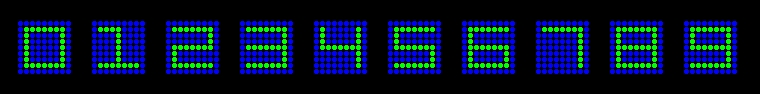
\includegraphics[width=0.99\textwidth]{pre_study_dataset}
    \caption[Straight Line Digits Dataset]{A novel dataset created to investigate the properties of modern deep learning architectures. The dataset consists of images of the numbers $0-9$, each image has a size of $9\times9$ pixels. The blue dots represent pixels with the value $0$, green dots represent pixels with the value $1$.}
    \figlbl{pre_study_dataset}
\end{figure}

The goal of this task is to predict the number (labels $0-9$) that is shown in the image.
This task is neither for humans nor deep learning architectures challenging.
However, it is simple enough to investigate the activations of neural networks and to search for net fragments.

The following example explains how net fragments could theoretically be built in this data set.
In total, the data set consists of $9$ basic lines, that can be composed to $10$ different digits.
A low-level net fragment could represent such a basic line and be composed to higher-level net fragments such as digits.
Figure \figref*{pre_study_components} visualizes these components (basic lines on the left, digits on the right).

\begin{figure}[h]
    \centering
    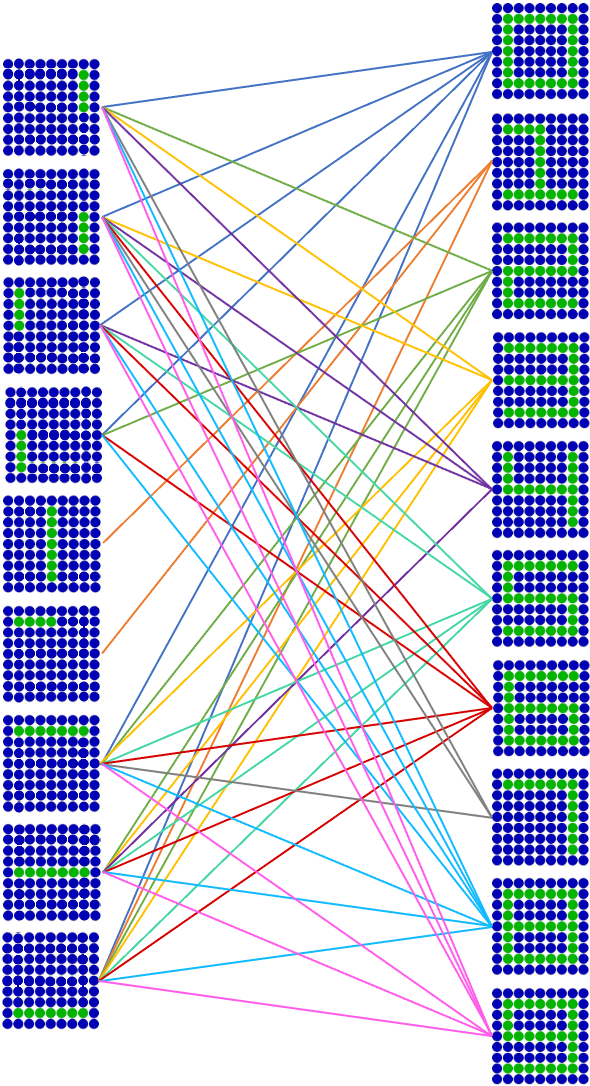
\includegraphics[width=0.99\textwidth]{pre_study_components}
    \caption[Line Types in Straight Line Digits Dataset]{A visualisation of all the lines (left) needed to compose the digits in the data set (right). The coloured lines in-between illustrate the relationship between the lines and the digits.}
    \figlbl{pre_study_components}
\end{figure}

Thereby, each low-level fragment can be part of one or multiple digits.
The composition can either take place across one or multiple layers.
The visualization in Figure \figref*{pre_study_components} can be interpreted as a composition across one layer, i.e. the low-level fragments are combined to high-level fragments within one step.

The composition can also take place across multiple layers. 
An exemplary composition of net fragments of the number $9$ across $4$ subsequent layers is shown in Figure \figref*{pre_study_composition}.
In this example, it is demonstrated that a fragment representing a digit can be composed of other fragments that also represent digits.
However, net fragments do not necessarily have to represent digits as shown in this example but can be a composition of multiple pixels without semantic.

\begin{figure}[h]
    \centering
    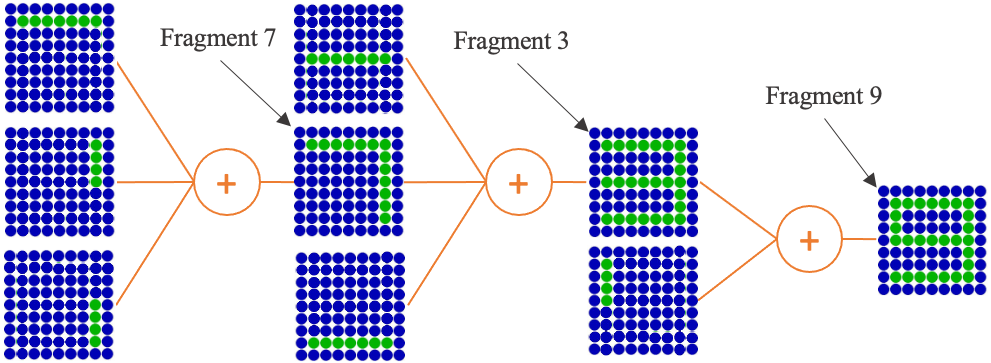
\includegraphics[width=0.99\textwidth]{pre_study_composition}
    \caption[Sample Net Fragment Composition]{A sample composition of the net fragment that could represent the digit $9$.}
    \figlbl{pre_study_composition}
\end{figure}

The fragments described so far are to be understood as an explanatory example.
A neural network might extract features in the first layers that do not correspond to vertical and horizontal lines and subsequently compose those features into more complex net fragments that are not as simple-to-interpret.
Meaning that looking for neurons of a (for us humans) simple to interpret meaning might be hard.
Regardless of what these net fragments represent, the network should have certain characteristics;
If a neuron or a group of neurons are part of a net fragment that represents a feature in the input, then these neuron(s) should be strongly active if the feature is present and not or only very weakly active if the feature is not present.
This leads to a sparse activation map and net fragments should only be active for digits with specific characteristics.
Furthermore, digits have common traits;
for example, the $7$ is contained in the $3$, the $3$ is contained in the $9$ and the $9$ is contained in the $8$.
The $1$, on the other hand, has nothing in common with the $4$, etc.
This means that at least one net fragment should be active for the $7$, $3$, $9$, and $8$ but not all net fragments that are composed to the digit $8$ should be active if the input depicts a $9$, $3$, or $7$.
The net fragments between the $1$ and $4$, on the other hand, should be completely different.
These properties should be visible in the activations of the network if it forms proper net fragments and are analysed in the following.

\section{Methods}\seclbl{pre_study_methods}
To investigate the emergence of net fragments, different deep learning models are trained.
The models are trained on a supervised classification task to predict the corresponding class of the images of the dataset shown in Figure \figref*{pre_study_dataset}.
The model's parameters are optimised by minimising the cross-entropy loss with the Adam optimizer \sidecite{Kingma2015AdamAM}.
The learning rate is $5 \cdot 10^{-4}$, the mini-batch size is $32$ samples and the model is trained for a total of $10$ epochs.

The models used have different feature extractors consisting of either convolutional (Conv.) layers (models no. $1$-$8$, no. $11$) or fully connected (FC) layers (models no. $10$) as shown in Table \tabref*{pre_study_models}.
Model no. $9$ has no feature extractor as the input images are so simple that they can be considered as features by themself, model no. $10$ uses a FC layer as feature extractor, and model no. $11$ has a Conv. layer with two hand-crafted kernels to extract horizontal and vertical lines as feature extractor.
After the feature extractor, all models have a similar ``head'' consisting of $2$ fully connected layers.
The feature extractor aims to extract certain features from the image, that are combined into higher-level net fragments in the first fully connected layer of the ``head'' and composed into predictions per class (i.e. net fragments corresponding to classes) in the last fully connected layer of the ``head''.
The first FC layer of the ``head'' consists of $12$ neurons.
The number of neurons was determined empirically by training various architectures and examining the number of active neurons.
It was found that there are always fewer than $12$ neurons active and that this capacity is therefore sufficient.
The last fully connected layer consists of $10$ neurons since this corresponds to the number of classes to predict.
The encoders of the models used are described in more detail in Table \tabref*{pre_study_models}.
The ``head'' is identical for all models and consists of a sequence of the following layers; FC ($12$ neurons) $\rightarrow$ ReLU $\rightarrow$ FC ($10$ neurons) $\rightarrow$ Softmax.

\begin{table}[h]
\newcolumntype{L}[1]{>{\raggedright\let\newline\\\arraybackslash\hspace{0pt}}m{#1}}
\newcolumntype{C}[1]{>{\centering\let\newline\\\arraybackslash\hspace{0pt}}m{#1}}
\newcolumntype{R}[1]{>{\raggedleft\let\newline\\\arraybackslash\hspace{0pt}}m{#1}}
    \tablbl{pre_study_models}
    \centering
	 \begin{tabular}{|l L{9cm}|} 
    	\hline
    	\textbf{No.} & \textbf{Encoder Description} \\
        \hline
		1 & Conv. Layer (kernel size=$3\times3$, channels=$2$) $\rightarrow$ ReLU $\rightarrow$ head \\ \hline
		2 & Conv. Layer (kernel size=$3\times3$, channels=$4$) $\rightarrow$ ReLU $\rightarrow$ head \\ \hline
		3 & Conv. Layer (kernel size=$5\times5$, channels=$2$) $\rightarrow$ ReLU $\rightarrow$ head \\ \hline
		4 & Conv. Layer (kernel size=$5\times5$, channels=$4$) $\rightarrow$ ReLU $\rightarrow$ head \\ \hline
		5 & Conv. Layer (kernel size=$3\times3$, channels=$2$) $\rightarrow$ ReLU $\rightarrow$ Conv. Layer (kernel size=$3\times3$, channels=$4$) $\rightarrow$ ReLU $\rightarrow$ head \\ \hline
		6 & Conv. Layer (kernel size=$3\times3$, channels=$4$) $\rightarrow$ ReLU $\rightarrow$ Conv. Layer (kernel size=$3\times3$, channels=$8$) $\rightarrow$ ReLU $\rightarrow$ head\\ \hline
		7 & Conv. Layer (kernel size=$3\times3$, channels=$2$) $\rightarrow$ ReLU $\rightarrow$ Max Pooling $\rightarrow$ Conv. Layer (kernel size=$3\times3$, channels=$4$) $\rightarrow$ ReLU $\rightarrow$ head\\ \hline
		8 & Conv. Layer (kernel size=$3\times3$, channels=$4$) $\rightarrow$ ReLU $\rightarrow$ Max Pooling $\rightarrow$ Conv. Layer (kernel size=$3\times3$, channels=$8$) $\rightarrow$ ReLU $\rightarrow$ head\\ \hline
		9 & head \\ \hline
		10 & FC ($9*9$ neurons) $\rightarrow$ ReLU $\rightarrow$ head \\ \hline
		11 & Hand Crafted Conv. Layer for vertical \& horizontal edge detection (kernel size=$3\times3$, channels=$2$) $\rightarrow$ ReLU $\rightarrow$ head \\
        \hline
    \end{tabular}
    \caption[Different Architectures for Preliminary Study]{A description of the different models used in the preliminary study.}
\end{table}

After each epoch, the model's weights are stored as well as the activations of each layer.
These vectors are visualized and investigated for net fragments.

Furthermore, the most relevant input features for a fully trained model are analysed.
This is done by freezing the model's parameters so that they cannot change.
Instead, an empty image is fed into the network and updated with backpropagation of error such that the probability for a given class is maximized.
This leads to an input image that has the highest probability to be predicted by the model as a specific class (e.g. generate the image that has the highest probability to be predicted as digit $3$ by the model).


\section{Results}\seclbl{pre_study_results}
All the models learn to classify these digits perfectly within a few epochs.
Interestingly, not only the accuracy reaches $100\%$ but some models also achieve a cross-entropy loss of $0.0$, meaning that they can find a global minimum.
However, the goal is not to achieve high accuracy but to exhibit net fragments.
It is not feasible to visualise all activations of all layers in this thesis.
Therefore, only the activations of the second last FC layer (i.e. the first FC layer of the ``head'') after the ReLU function are shown.
Since the last layer contains the net fragments that depict classes, this is the layer with the highest-level fragments.
Furthermore, it is the only layer that has a global view on the input, i.e. can access all the features extracted by the encoder\sidenote{convolutional layers only consider a local neighbourhood by sliding a kernel over the input (c.f. \secref{cnns})} (except for the encoder consisting of FC layers only).
Some higher-level net fragments should be visible in this layer, which are subsequently composed in the last layer to net fragments corresponding to classes.
Interested readers who want to investigate the activations from all layers, as well as the network weights by themselves, can view an interactive visualisation at \url{http://160.85.252.38:8501}.

\figref{pre_study_activations} shows the activations of the first fully connected layer in the ``head'' of the different models.
The FC layer has $12$ neurons whose activation is indicated along the vertical axis (per model), and the horizontal axis depicts the activation of the same neuron for the classes $0$-$9$.
For example, the circle in the top left corner indicates the activation of the first neuron for class $0$, the circle in the top right corner the activation of the first neuron for class $9$, and the circle in the bottom left corner the activation of the last neuron for class $0$.
Blue circles show activations that are exactly $0$, red circles are low activations $>0$, and green circles represent strong activations\sidenote{activations $<0$ do not exist because they are set to exactly $0$ by the ReLU function}.

It can be seen in the visualization that none of the models utilises all $12$ neurons and certain neurons are always inactive regardless of the class.
Also, no obvious net fragments can be identified;
Most neurons are always similarly strongly active regardless of the class.
If net fragments are formed, however, the neurons of a fragment would have to be strongly active in the presence of certain features and weakly active otherwise.
Such behaviour is not observable in these activations.

Furthermore, some digits are very similar and differ in only two pixels.
Some examples are the digit pairs $5$ and $6$, $8$ and $9$, $0$ and $8$, or $3$ and $9$.
However, when the activations of the corresponding classes are compared, it is obvious that almost always all activations change a little bit, and not one neuron is turned on or off depending on the presence of these two pixels.

\begin{figure}[h]
    \centering
    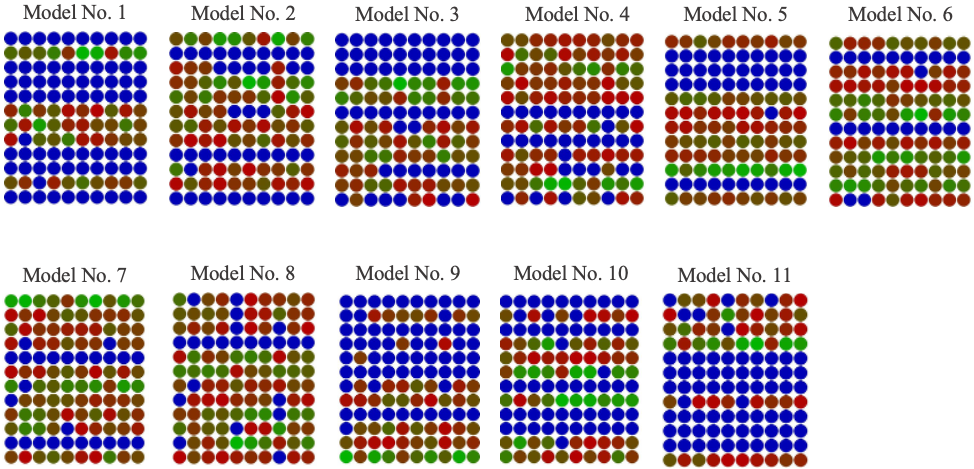
\includegraphics[width=0.99\textwidth]{pre_study_activations}
    \caption[Network Activations for Straight Line Digits Dataset]{The activations of the first fully connected layer in the ``head'' of the different networks. For each model, the activity of the $12$ neurons is shown for each class (activations along the vertical axis, classes along the horizontal axis). Red means low activation, green means high activation, blue means activation is off (i.e. $0$).}
    \figlbl{pre_study_activations}
\end{figure}

%It can also be observed that roughly the same neurons are always active.
%For different classes, however, these neurons do not switch on or off, but the strength of the activity changes.

\figref{pre_study_inputs_max} visualizes the input that maximizes the probability for each class.
It is obvious that all models focus on the wrong features and it can be assumed that these networks would not be robust to slight perturbations in the input.
This also indicates that net fragments are not present in current deep learning models (or at least not to the desirable extent);
if a class-level net fragment is composed of several lower-level net fragments, then some of these lower-level net fragments have to be active.
Since these lower-level net fragments represent specific input features, corresponding pixel constellations should be visible in this visualisation.
However, since these rather random-looking pixel combinations maximise the probability of predicting a specific class, this suggests that pixel combinations are not composed into hierarchically more complex net fragments.

\begin{figure}[h]
    \centering
    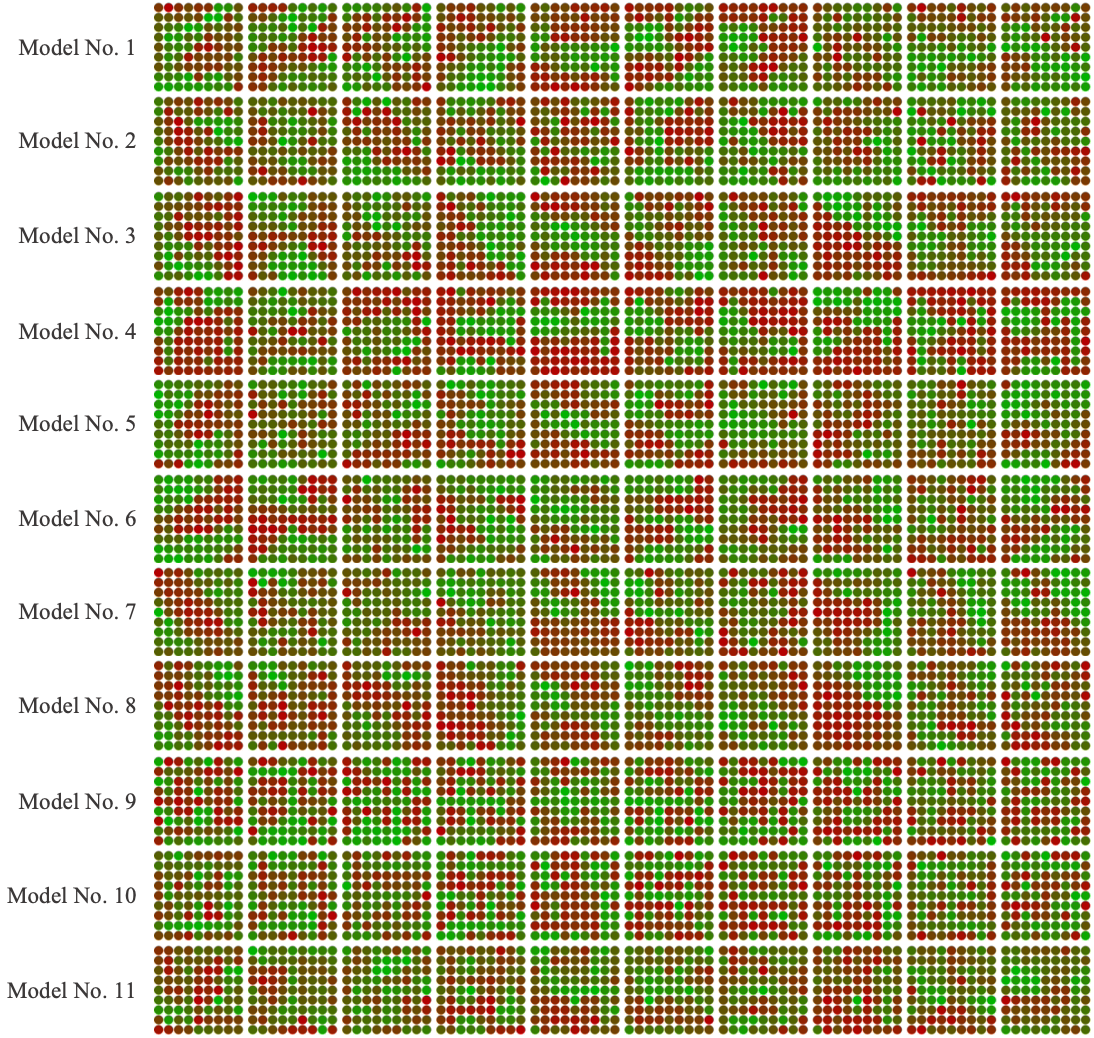
\includegraphics[width=0.99\textwidth]{pre_study_inputs_max}
    \caption[Inputs that Maximize the Class Output Probability]{The inputs that maximize the probability that the different models predict a specific class. For example, the image in the top left corner maximizes the probability that model number $1$ predicts that this is class $0$ (digit $0$).}
    \figlbl{pre_study_inputs_max}
\end{figure}


\section{Conclusion}\seclbl{pre_study_conclusion}
Different architectures have been trained on a very simple and therefore easily interpretable data set.
It was found that certain neurons are never active, while the active neurons usually remain active regardless of the class of the input data and only change their activity slightly.
Net fragments, on the other hand, rely on being strongly active when the corresponding feature they represent is present in the input and are weakly active or not active at all when it is not present.
Therefore, I argue that deep learning architectures do not comprise net fragments by default.

This assumption is further strengthened by the visualisation of the input that maximises the probability per class.
If a class is represented by a net fragment and this net fragment is composed of other net fragments, then some of these lower-level fragments would have to be active.
Such a set of low-level net fragments can directly be mapped to a set of pixels that has to be active.
However, since the input does not contain a meaningful (sub-) set of active pixels, it can be assumed that these lower-level fragments are either not present or at least do not represent any meaningful features.




\setchapterpreamble[u]{\margintoc}
\chapter{Methods}\chlbl{methods}
%% methods.tex
This chapter describes the methodology used.
A large part of the contribution of this thesis consists of identifying appropriate findings from neuroscience and adapting them to a deep learning setting.
This identified concept and the link between the two disciplines is described in chapter \secref*{neuro_concepts}.
It should be noted that this section presents only one possible interpretation for the implementation of neuroscientific concepts in the context of deep learning and that alternative interpretations might also be promising.
Afterwards, two possible implementation approaches are described, which differ mainly in the type of local self-organisation.
These types of self-organisation are referred to as horizontal and vertical self-organisation and are described in Section \secref*{vertical_self_org} and Section \secref*{horizontal_self_org} respectively.




\section{Neuroscientific Concepts}\seclbl{neuro_concepts}
It is known that large parts of the human brain are self-organizing \sidecite{kelso1995dynamic}.
Recently, renowned scientists \sidecite{von_der_Malsburg_Stadelmann_Grewe_2022} put forward the hypothesis that this process of self-organization is the key mechanism of natural intelligent systems such as the human brain.




Dresp \sidecite{Dresp2020SevenPO} describes seven clearly identified properties of self-organization in the human brain: (i) modular connectivity, (ii) unsupervised learning, (iii) adaptive ability, (iv) functional resiliency, (v) functional plasticity, (vi) from-local-to-global functional organization, and (vii) dynamic system growth.

However, it is not obvious how these insights from neuroscience can be integrated into a deep learning framework.
One interpretation of self-organization may be that instead of optimizing the entire network by statistical learning for a single task (i.e. using backpropagation), local optimization based on local input data takes place.
The suitability of backpropagation for explaining how the brain learns was questioned soon after it was published \sidecite{Crick_1989, Grossberg_1987}.
Many alternative and biologically more plausible algorithms have been proposed in recent years such as the feedback alignment (FA) algorithm \sidecite{Lillicrap_Cownden_Tweed_Akerman_2014}, contrastive Hebbian learning \sidecite{Movellan_1991}, generalized recirculation \sidecite{O_Reilly_1996}, as well as target propagation (TP) and its variants \sidecite{Le__Cun_1986, hinton2007backpropagation, Lee_Zhang_Fischer_Bengio_2015}.
However, Bartunov et al. \sidecite{Bartunov_Santoro_Richards_Marris_Hinton_Lillicrap_2018} have shown that these algorithms do not scale to large vision datasets such as ImageNet \cite{deng2009imagenet} and only work for smaller datasets such as MNIST \cite{MNIST} and CIFAR-10 \cite{cifar_10}.
The biologically most plausible learning algorithm is Hebbian learning (c.f. Section \secref{hebbian}).
However, even tough I obtain some promising results in preliminary results with Hebbian learning (c.f. Appendix \secref{exp_hebb_learning}), this algorithm doesn't seem to be well suited to learn good image representation if a network is trained from scratch.

TODO: Füge FF-Algorithmus von Hinton hinzu

Another interpretation of self-organization within neural network is that the networks adapts its structure during training.
According to von der Malsburg et al. \cite{von_der_Malsburg_Stadelmann_Grewe_2022}, neurons form net-fragments (a.k.a. sub-networks) that represent objects with different levels of abstraction within an image (c.f. section \secref{natural_intelligence}).
For example, some net-fragments may represent shapes and structures while a multitude of such net-fragments together represent objects such as persons or entire scenes.
Thus, self-organization could be the algorithm to form net-fragments that represent objects independent of their transformation.

Such a mechanism to form networks that can capture scenes in the form of net-fragment has not been successfully implemented in deep learning nor neurocomputing systems.
This thesis aims to develop a learning paradigm that explicitly foster creation of net-fragments that represent objects independent of their transformation.
... TODO ...




% TODO: VON HIER SCHIEBE IN NEUES KAPITEL -> ABSTRAKTE KONZEPTE von Neuroscience IN DL Übertragen
In addition to these well-defined terms, there are various biological principles observed in the field of Neuroscience that are either not completely understood or it is unclear how they can be incorporated into artificial networks.
The concepts relevant for this thesis are discussed in the following.
However, due to the aforementioned challenges, no definition of these principles is given but rather my own interpretation in the context of this work.

A central concept of this work are sub-networks.
Typically, in current DL architectures for computer vision, an encoder is used to compute object representations in a latent space.
Thus, the output of a single layer can be understood as an object representation\sidenote{this is also true for image classification: Usually, a classification head consisting of fully connected layers and subsequent softmax activation is used after an image encoder}.
According to von der Malsburg et al. \cite{von_der_Malsburg_Stadelmann_Grewe_2022}, biological sub-networks span multiple layers.
This concept is interpreted in such a way that the latent representations should not be extracted from the last layer of an encoder but from several layers.
While the first layers of an image encoder contain more local information, the last layers contain very global information.
It is known from speech representation learning that different layers capture different speech information \sidecite{Chung_Hsu_Tang_Glass_2019}.
For example, the first layers contain more information to distinguish speakers, while representations in later layers provide more phonetic content.
However, such information seems to be poorly exploited in computer vision architectures.
One could argue that skip connections in segmentation networks \sidecite{Ronneberger_Fischer_Brox_2015} exploit such information.
While this may be true to some extent, information from previous layers is still squeezed into a feature vector and can be poorly exploited by downstream tasks.
TODO: Umsetzung Sub-Networks beschreiben

In addition to forward connections, lateral connections are also located in visual cortex \sidecite{gilbert1990lateral}.
Thus, the biological neurons are not only connected to the neurons in the subsequent layer but also within the same layer.
TODO: Je nach Umsetzung erklären, wie lateral connections in ANN interpretiert werden (+ Zeichnung einfügen)

Another principle that seems important in biological neural networks is sparsity.
Over time, the number of active neurons in the visual cortex decreases.
For example, in the visual cortex of mice are more than 75\% of the neurons active before the first opening of the eyes, 36\% after the opening of the eyes and only 12\% in adulthood \sidecite{Rochefort_Garaschuk_Milos_Narushima_Marandi_Pichler_Kovalchuk_Konnerth_2009}.
Thus, a sparsification of neuronal activations takes place through visual experience.
In the field of deep learning, sparisty is often interpreted in two different forms; sparse weight matrices and sparse activation matrices.
Sparse weight matrices are often chosen to make models smaller or to increase inference speed \cite{Louizos_Welling_Kingma_2018, Hoefler_Alistarh_Ben_Nun_Dryden_Peste_2021}.
From a biological point of view, this process of first creating a large network and then shrinking it is obviously not plausible\sidenote{otherwise we would have a large brain at the beginning, which becomes smaller by factors in the course of time}.
Sparse activations, on the other hand, can increase robustness \cite{Panousis_Chatzis_Theodoridis_2021}.
Intuitively, sparse activations enforce that only the most relevant information is passed to the subsequent layer.
Furthermore, sparse activations can help to obtain sub-networks.
Objects are represented in sub-networks (i.e. in multiple layers).
If all neurons in all layers are always active, then object representations cannot be extracted from sub-networks, since it is unclear which activation pattern represents which object.
If, on the other hand, only a fraction of the neurons are active, then certain neuron combinations can infer objects.
TODO: Umsetzung Sprase Activations beschreiben

A biological intelligent organism has an embodiment and can interact with the world.
At the same time, the visual system perceives continuous input all the time (except when sleeping or blinking).
As a result, the visual signal changes only minimally from one perceived frame to the next over a long course of time.
An ANN, on the other hand, is typically trained on samples that have little relation to each other.
When the system is trained on images, each frame is different; with videos, each sequence of frames is different.
A continuous input might help to get better representation of objects through self-supervised learning.
If an input is continuous and shows the same object from different angles or in different transformations (e.g. stretching) and it can be inferred that it is the same object then the object representations derived from this continuous stream can be homogenized.
These principles are already applied to some extent by self-supervised learning systems for computer vision.
In contrastive learning, a popular form of self-supervised learning, two different views are derived from one image by data augmentation, and their representations are then pushed closed together in the feature space \sidecite{chen2020simple, chen2020big, caron2020unsupervised}.
However, this paradigm is still quite limited since only two views of the same scene and not the continuous transformation of an object are presented to the learning system.
TODO: Umsetzung beschreiben


\section{Vertical Self-Organization}\seclbl{vertical_self_org}
2 Arten von Loss: 1x Diversity + Sparsity, 1x MI zwischen vorherigem und nachfolgendem Layer

\section{Horizontal Self-Organization}\seclbl{horizontal_self_org}

\setchapterpreamble[u]{\margintoc}
\chapter{Results}\chlbl{results}
This chapter presents the results of the conducted experiments. First, an overview of the results achieved with the entire system is provided. Subsequently, individual components of the system are examined in more detail.
The code and documentation are made publicly available. Further information can be found in the appendix \chref{online_sources}.

\section{Entire System}
%
\begin{figure}[h]
    \centering
    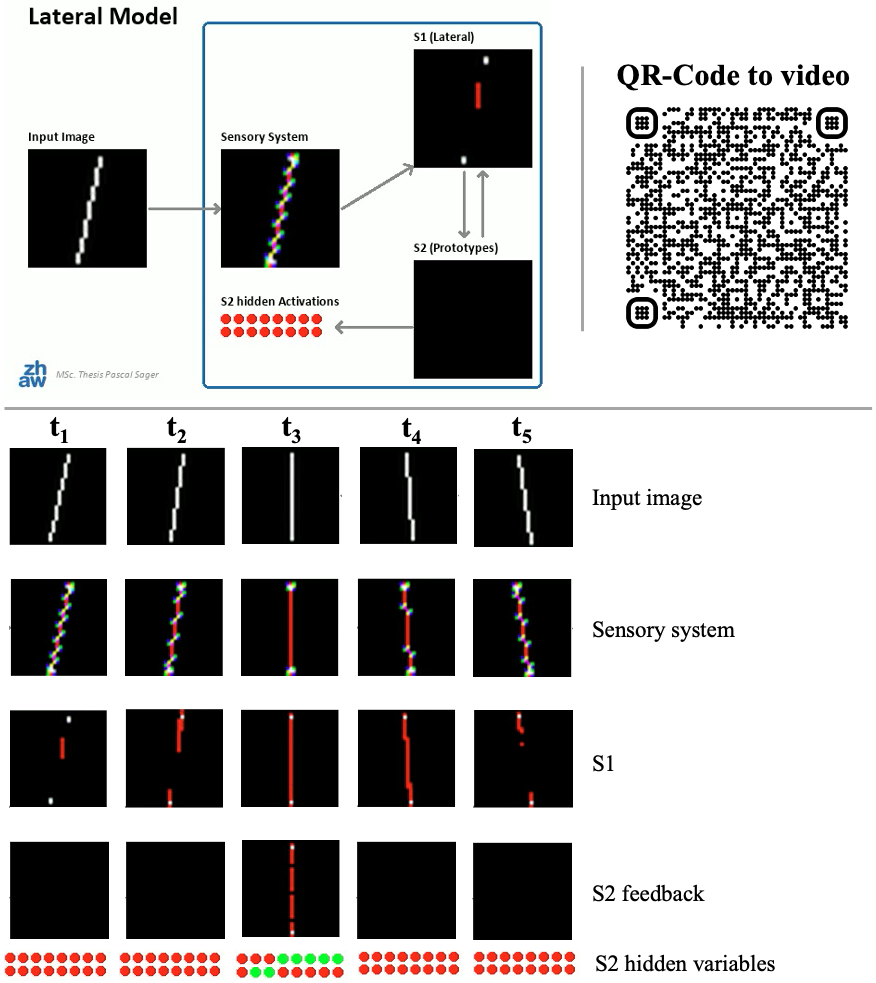
\includegraphics[width=0.99\textwidth]{r1_overview}
    \caption[Frames of a video visualising the model's activations]{Frames of a video visualising the model's activations. At the top of the image, an actual video frame and a QR code linking to the video are shown. At the bottom of the image, the changing network activations over time are visualised.}
    \figlbl{r1_overview}
\end{figure}
%
An overview of the entire system is provided in \figref{r1_overview}.
This image is derived from a video available online at \href{https://sagerpascal.github.io/lateral-connections/results/final_results.html#video-visualisations}{sagerpascal.github.io/lateral-connections} or with the QR code on the top right of the figure.
For a detailed explanation of the components shown in the video, please refer to appendix \secref{result_video}.
The video shows the network's activations for a straight line rotated counterclockwise around its centre.
In the lower part of \figref{r1_overview}, a series of five network states is shown shortly before and after a vertical line is reached.

The network has only been trained on vertical, horizontal, and diagonal lines.
Therefore, many lines fed into the network in this video represent unknown objects\sidenote{With projection fibres, such transformed objects instances should be mapped to the same prototype. However, the memory used cannot deal with such transformations.}.
Nevertheless, \emph{S1} still detect some learned patterns, such as multiple pixels aligned vertically, horizontally, or diagonally.
Therefore, it can provide lateral support between local pixel groups representing such a local pattern.
The closer the input becomes to a learned pattern, the bigger the lateral support.
At time $t_3$, the input corresponds to a vertical line as observed during training.
In that case, all pixels receive enough lateral support to remain active.

For the conducted experiments, \emph{S2} does not map the net fragments to a reference frame but acts as a memory of learned objects.
As long as the net fragments represent an unknown pattern, no latent cells in \emph{S2} are activated and no feedback to \emph{S1} is provided.
However, when the net fragments in \emph{S1} correspond to a learned pattern, \emph{S2} provides feedback and further increases certainty in \emph{S1}.
When replacing the memory used to simulate \emph{S2} with projection fibres, the feedback should be even better, as \emph{S2} will be able to detect transformed objects.

The network's behaviour is as expected: \emph{S1} builds net fragments based on well-known patterns observed during training.
All input features observed during training receive full lateral support.
Moreover, images not seen during training also contain local patterns similar to those from the training data and, therefore, still receive local support.
\emph{S2} responds to patterns stored in its memory, only providing support to \emph{S1} for objects seen during training.

Furthermore, all samples seen during training have automatically been saved in \emph{S2}.
The system is able to produce net fragments that roughly reassemble the input from the sensory system.
However, the net fragments are more robust than the sensory system, as shown in the following sections.

\subsection{Effect of Noise}
%
\begin{figure}[h]
    \centering
    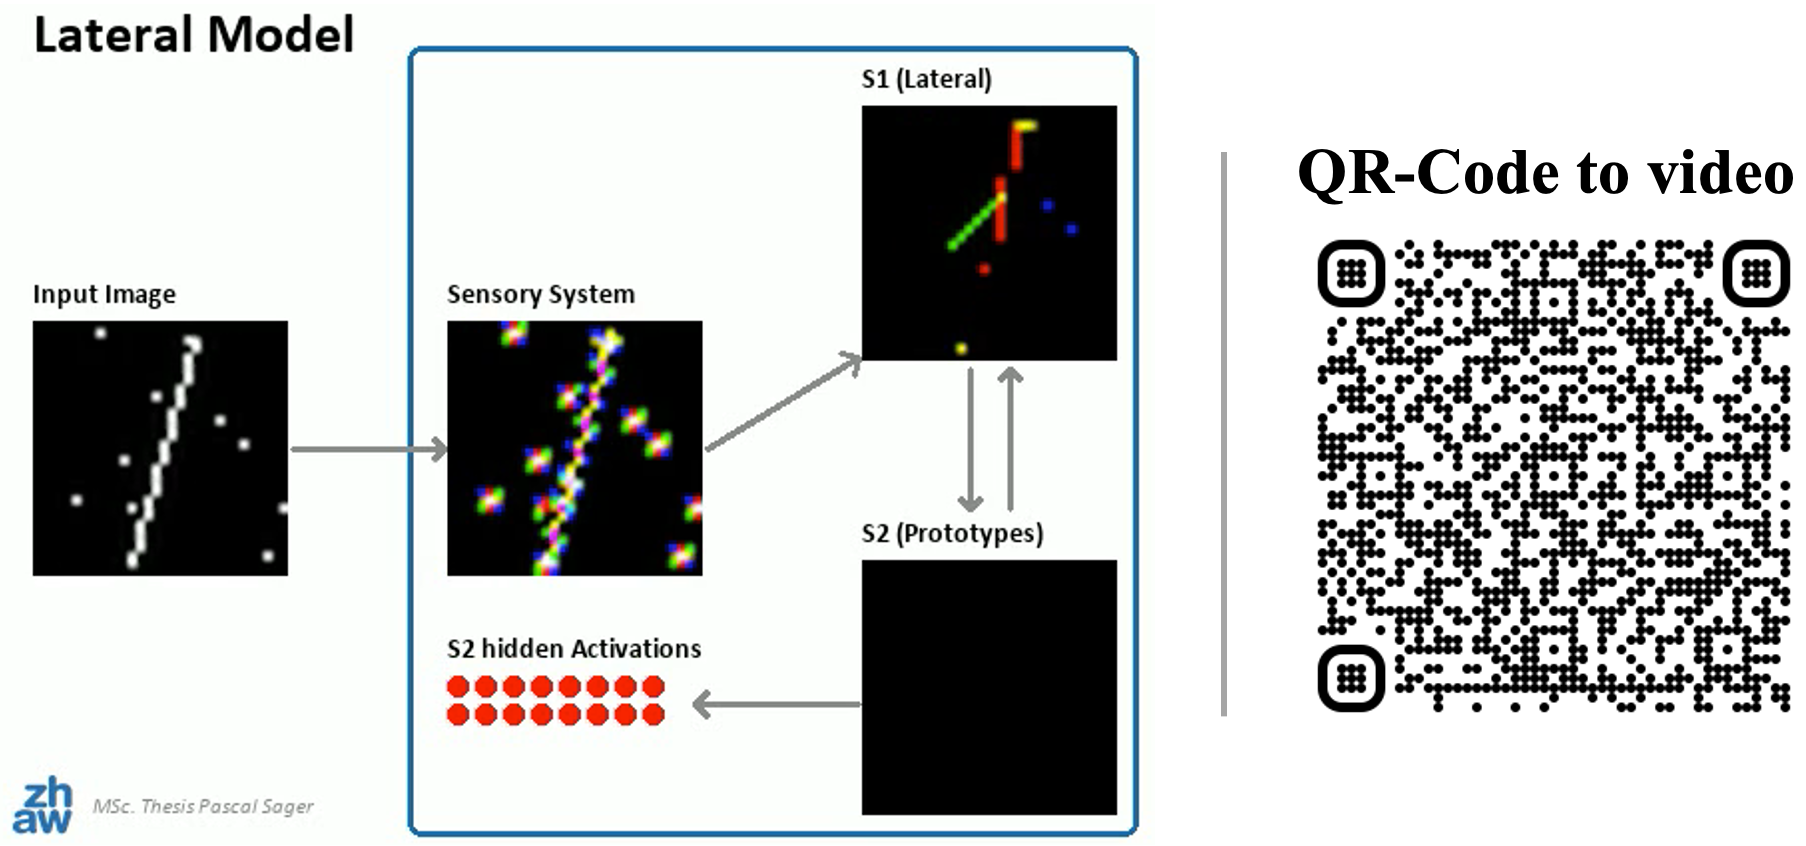
\includegraphics[width=0.99\textwidth]{r2_overview}
    \caption[Video visualising the network's behaviour with noise in input]{A frame of a video visualising the network's behaviour if noise is added to the data. The QR code on the right links to the corresponding video.}
    \figlbl{r2_overview}
\end{figure}
%
\figref{r2_overview} refers to a video demonstrating the network's behaviour when noise is added to the input data.
The noise is generated by randomly flipping a pixel in the input data from $0$ to $1$ or vice versa with a probability of $0.005$.

To assess the network's ability to deal with noise, the same input is fed into the model twice: once with and once without noise. The activations of \emph{S1} for these two versions of the input image are compared, and the percentage of feature cells that are initially triggered by the introduced noise but subsequently deactivated due to insufficient support is measured.

This analysis shows that the system can remove about $71.2\%$ of the noise from the input data. However, this effectiveness is mainly because a single noise pixel triggers $3$ cells in each feature channel of the sensory system, resulting in $12$ active cells. After building net fragments, only the cells at the centre of the four feature channels remain active, giving the impression that the noise has been removed while, in reality, it only has been reduced.

\begin{figure}[h]
    \centering
    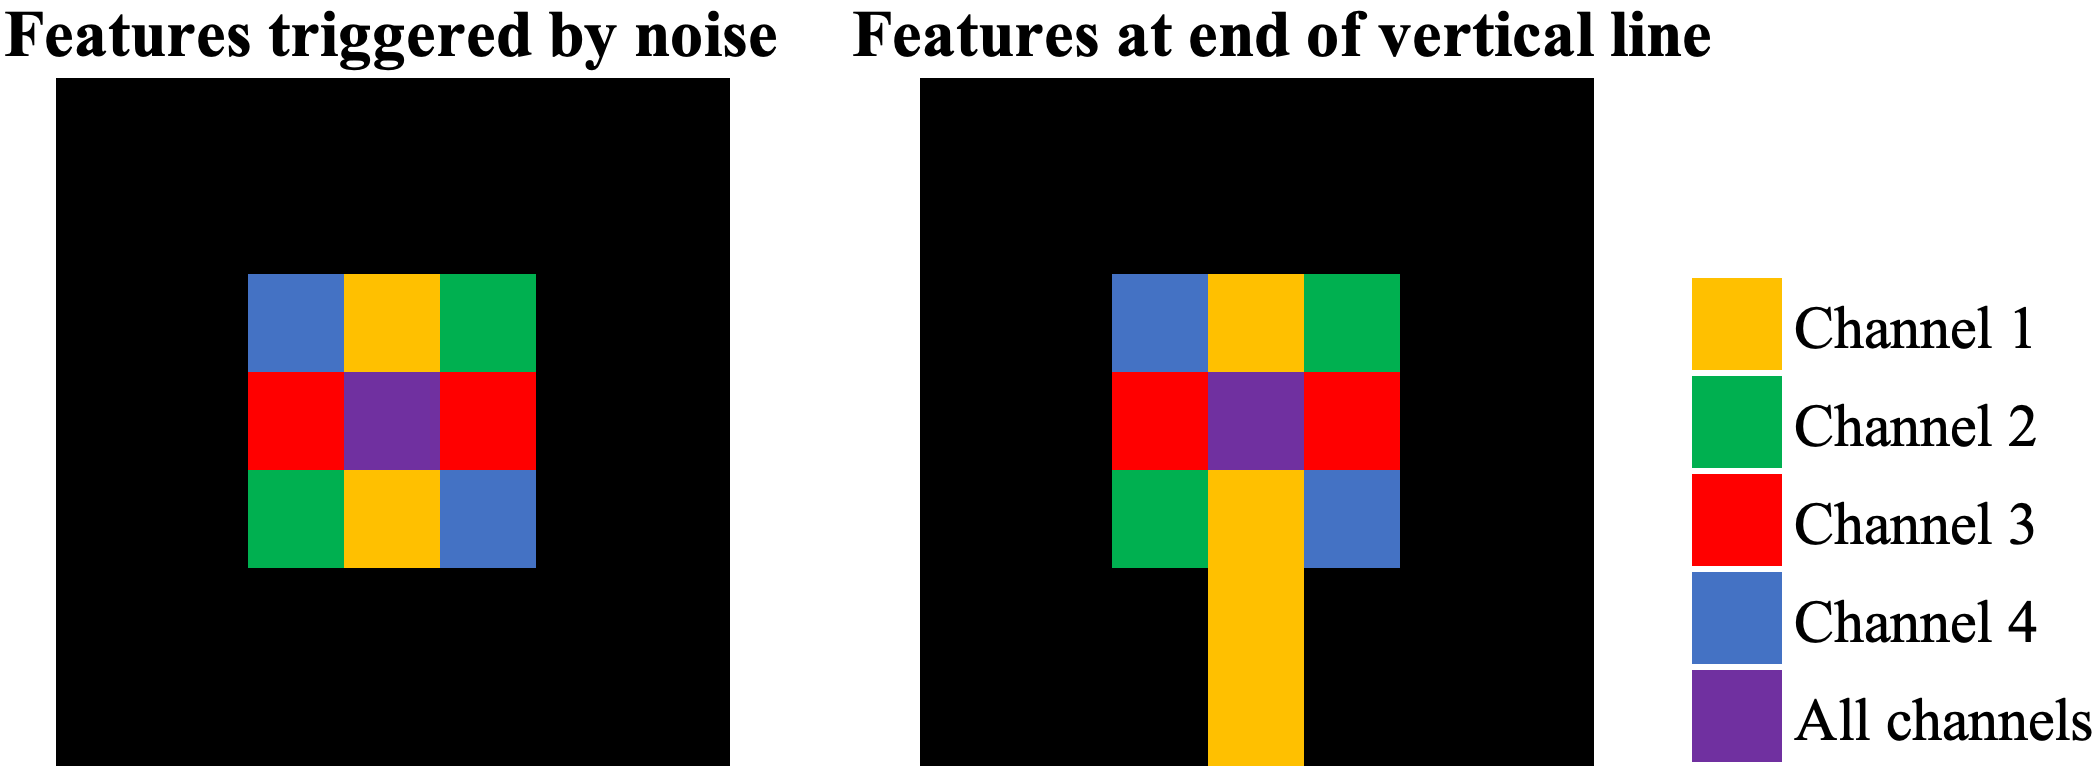
\includegraphics[width=0.79\textwidth]{features_noise_data}
    \caption[Features triggered by noise]{The features triggered by noise (on the left) compared with the features triggered by a line end (on the right).}
    \figlbl{features_noise_data}
\end{figure}
%
In fact, only in $23.8\%$ of the cases is noise in the input completely removed.
Several reasons contribute to the difficulty of obliterating noise: First, noise can be located close to the line or other noise and thus receives lateral support from other cells. Second, when observing noise in the input, the sensory system triggers activations in all feature channels similar to activations found at line ends as visualised in \figref{features_noise_data}.
As a result, activations triggered by noise are very similar to learned patterns. Therefore, these cells support each other and cannot be adequately filtered by the system.
Overall, this behaviour is to be expected, and noise should only be filtered out if it is significantly different from learned patterns.

Although the noise cannot be completely filtered out, the net fragments are still accurately mapped to the correct prototype in \emph{S2}. Thus, the system still correctly interprets the input despite the noise.

\subsubsection{Noise per Channel}
%
\begin{figure}[h]
    \centering
    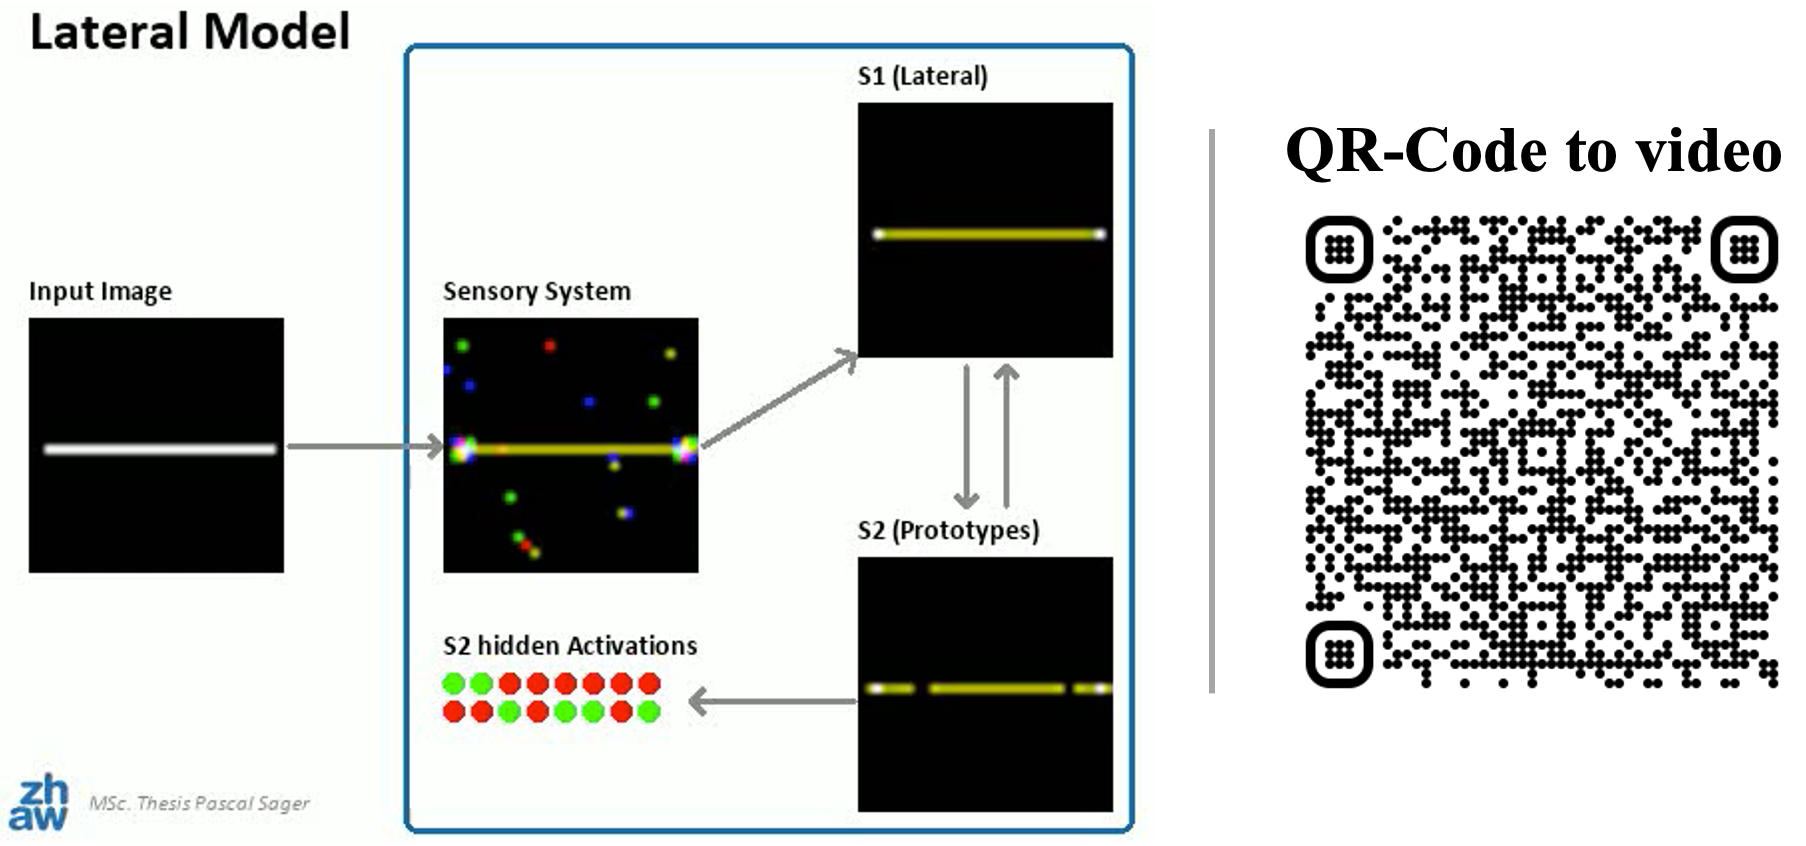
\includegraphics[width=0.99\textwidth]{r3_overview}
    \caption[Video visualising the network's behaviour with noise in the feature channels]{A frame of a video visualising the network's behaviour if noise is added to the feature channels. The QR code on the right links to the corresponding video.}
    \figlbl{r3_overview}
\end{figure}
%
In this section, it is investigated whether noise can be filtered when there is no correlation between the locations of the noise within the feature channels.
Thus, the noise does not correspond to learned patterns anymore.
Therefore, noise is not added to the input data but to each feature channel of the sensory systems' output separately.
This experiment is considered more relevant for real-world scenarios, as future systems that deal with real-world data will have a much larger number of input channels and more diverse patterns, making it unlikely that noise resembles a learned pattern that the network considers valid.

\figref{r3_overview} refers to a video demonstrating the networks' behaviour when noise is added to each feature cell with a probability of $0.005$.
In this case, about $91.7\%$ of the noise is removed, demonstrating the network's high robustness to such perturbations.
The noise that is not removed is the noise that is very close to the actual line and therefore receives support from a valid object.

\subsection{Discontinuous Line}
%
\begin{figure}[h]
    \centering
    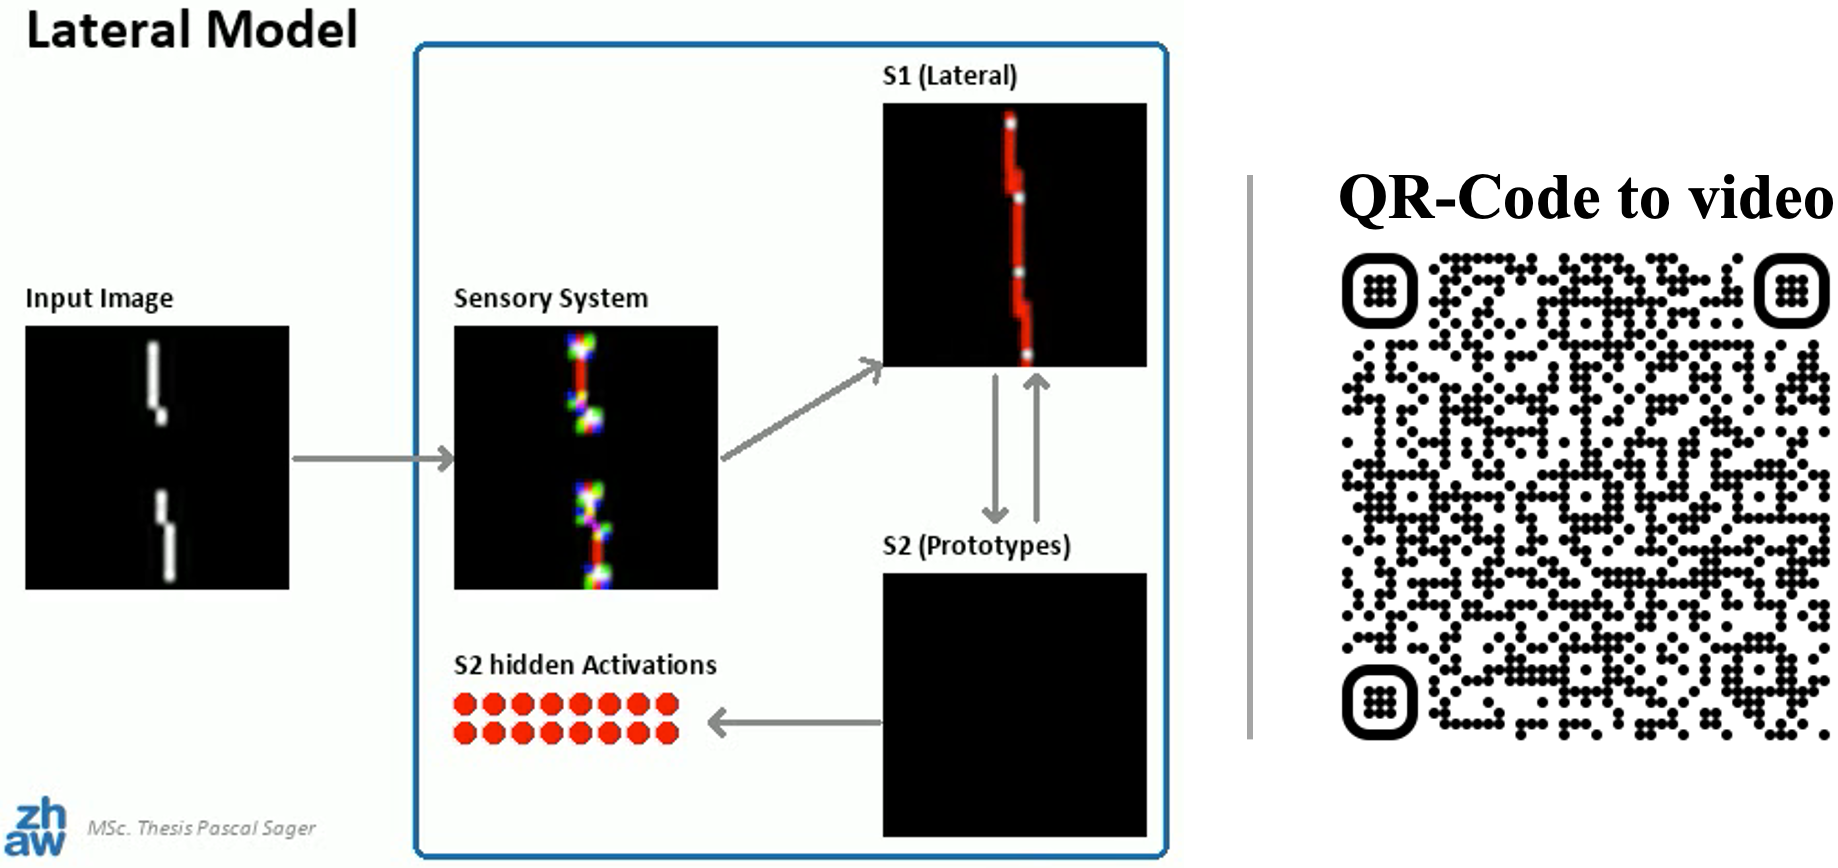
\includegraphics[width=0.99\textwidth]{r4_overview}
    \caption[Video visualising the network's behaviour for discontinuous lines]{A frame of a video visualising the network's behaviour for discontinuous lines. The QR code on the right links to the corresponding video.}
    \figlbl{r4_overview}
\end{figure}
%
Net fragments \sidecite{von_der_malsburg_theory_2022, von_der_malsburg_concerning_2018} can not only reduce noise but also recreate occluded objects.
This phenomenon is demonstrated by analysing the network's behaviour if a discontinuous line is fed into the network.
In \figref{r4_overview}, a QR code is contained linking to a video demonstrating that \emph{S1} is able to reconstruct lines that are interrupted by up to $8$ pixels.

In the experimental setup, the centre of the line is detected, and a varying number of pixels starting from the centre are intentionally switched off.
The feedback from \emph{S2} is switched off so that only the reconstruction based on net fragments within \emph{S1} is tested.
Remarkably, the \emph{S1} consistently succeeds in reconstructing the original training input when up to $6$ pixels are removed. Furthermore, in many cases, it can reconstruct lines with up to $8$ pixels missing, although it fails with more than $8$ pixels removed.

The extent to which the network can reconstruct discontinuous lines depends on the range of lateral connections $n_l$. As expected, increasing the value of $n_l$ allows \emph{S1} to reconstruct lines with more missing pixels, improving its performance in recovering objects.
However, $n_l$ should not be too large so that \emph{S1} build net fragments based on local features (c.f. \secref{neuroscience_findings_net_fragments}).

In the conducted experiments, the lateral range is set to $n_l=11$.
The impressive ability to reconstruct up to $8$ missing pixels with this setting suggests that recreating occluded patterns works effectively.


\subsection{S2 Feedback}\seclbl{results_s2_feedback}
In the following, feedback from \emph{S2} is additionally incorporated in \emph{S1}, and it is analysed if \emph{S1} can efficiently utilise it to reconstruct lines.
Please note that not all aspects from \emph{S2} are implemented, and it is a memory that returns stored net fragments if they are similar to an observation.
Therefore, it only works for the examples the network encountered during the training process, i.e. for vertical, horizontal, and diagonal lines.

\begin{figure}[h]
    \centering
    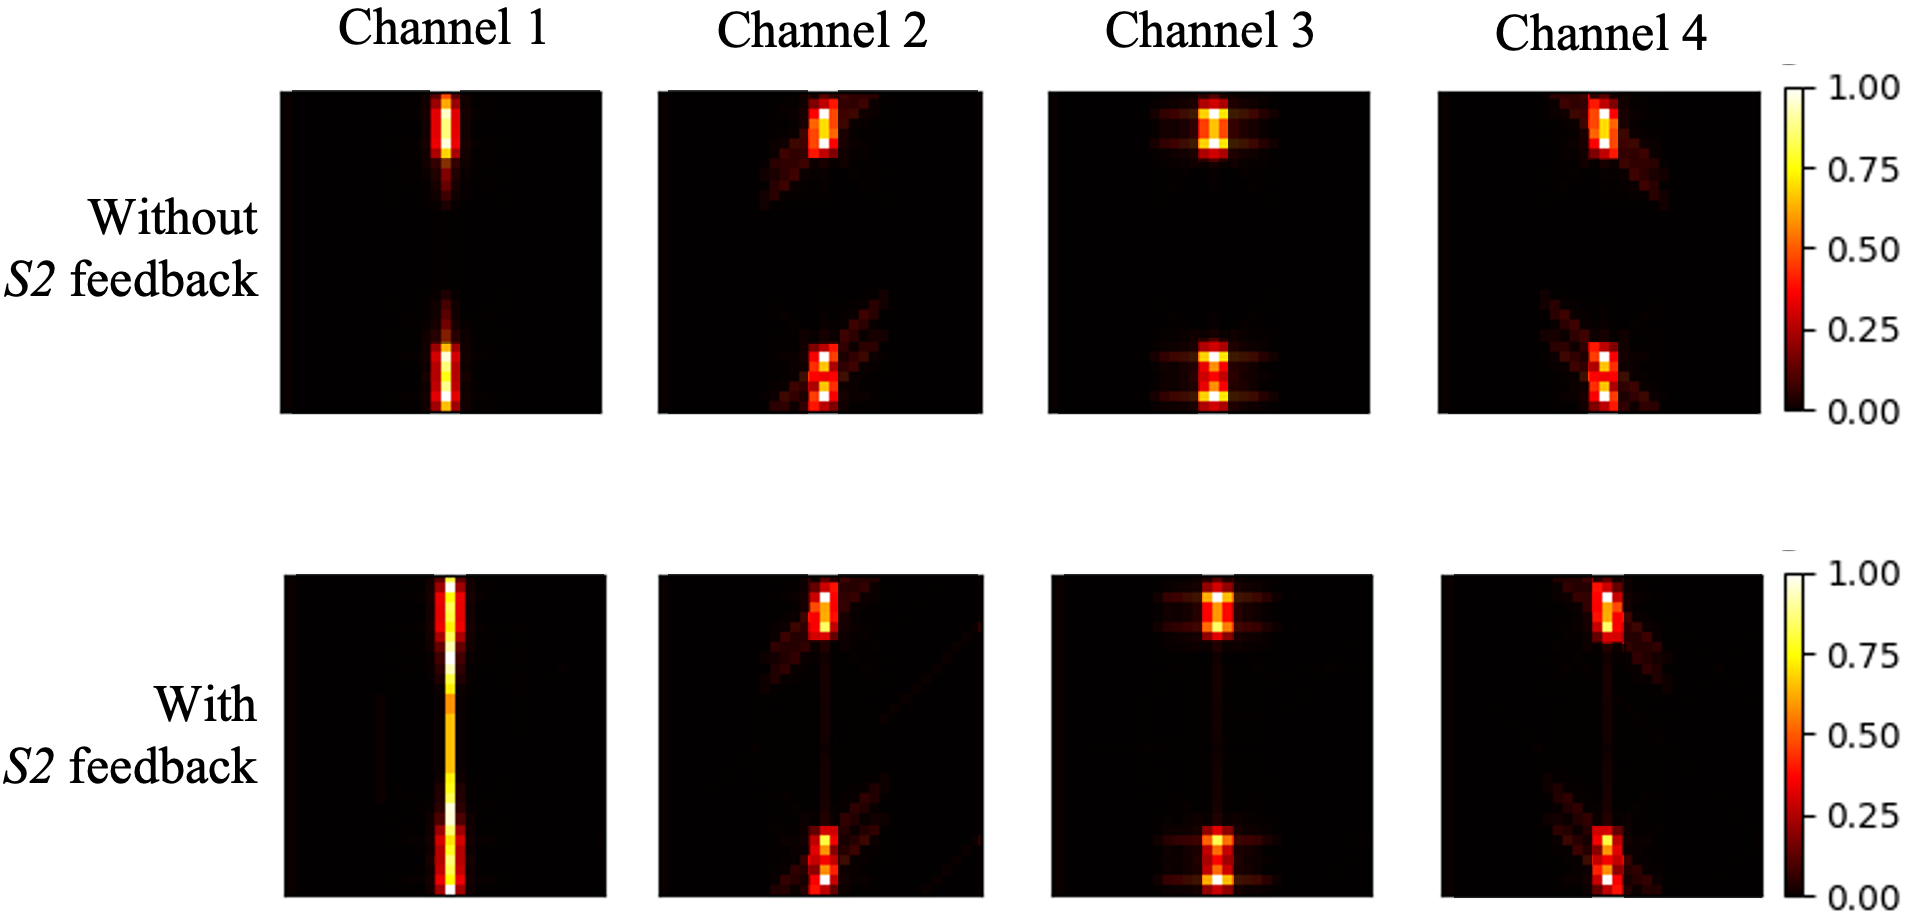
\includegraphics[width=0.99\textwidth]{s2_feedback_heatmap}
    \caption[Activation probabilities with and without \emph{S2} feedback]{The activation probabilities per cell across all four channels with and without feedback from \emph{S2}. The input is a discontinuous vertical line with $20$ pixels missing.}
    \figlbl{s2_feedback_heatmap}
\end{figure}
%
In \figref{s2_feedback_heatmap}, the activation probabilities for all cells across the four output channels for a vertical line with $20$ missing pixels are visualised.
The top row shows the probabilities when no feedback form \emph{S2} is incorporated, and the bottom row the probabilities after the feedback is incorporated.

As visible in the top row of \figref{s2_feedback_heatmap}, without incorporating feedback from \emph{S2}, the line cannot be fully reconstructed using lateral connections in \emph{S1}, as $20$ of missing pixels exceeds the range of lateral connections. However, \emph{S2} is still able to map the line with missing pixels to the correct prototype and provide appropriate feedback. After the feedback is incorporated, the activation probabilities for the entire vertical line increase significantly. Especially in the middle section of the first channel, the activation probabilities increase from $0\%$ to approximately $65\%$.

When a continuous vertical line is fed into the system, the activation probability in the middle section of the line is above $90\%$.
This high probability aligns with the fact that the sensory signal and the memory's feedback are consistent.
However, when the memory expects activations that are not detected by the sensory system (e.g. due to the missing pixels), the activation probability decreases. This behaviour reflects meaningful modelling of the network's uncertainty when integrating feedback from \emph{S2} while encountering occluded objects.

In conclusion, the feedback from \emph{S2} can be effectively incorporated into \emph{S1}.
It helps to deal with occluded objects and creates stability in net fragments, even when the sensory system does not detect (occluded) parts of the object.



\section{Model Weights}
%
\begin{figure}[h]
    \centering
    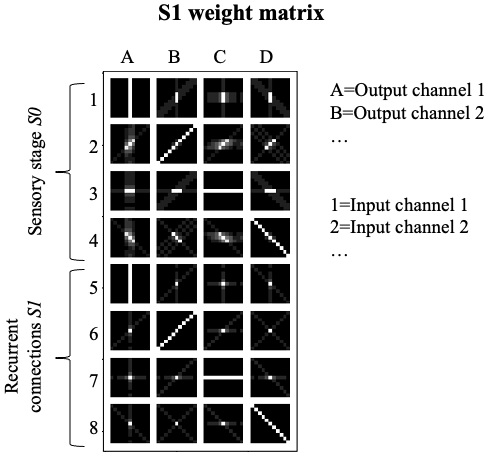
\includegraphics[width=0.79\textwidth]{S1_weight_matrix}
    \caption[Weight matrix of \emph{S1} after training]{The weight matrix of \emph{S1} after training.}
    \figlbl{S1_weight_matrix}
\end{figure}
%
The weight matrix of \emph{S1}, which contains the strength of the learned lateral connections, is discussed in the following section.
In \figref{S1_weight_matrix}, the learned weights are visualised. 
The input of \emph{S1} consists of four channels from the sensory stage (rows labelled as $1$-$4$) and four channels from recurrent connections (labelled as $5$-$8$).
\emph{S1} produces four output channels, and the kernels contributing to each output channel are depicted in columns labelled from $A$ to $D$.
Each output channel specialises in a different type of line: Output channel $A$ focuses on vertical lines, channel $B$ on diagonal lines with a positive slope, channel $C$ on horizontal lines, and channel $D$ on diagonal lines with a negative slope.

An analysis of output channel $A$, which focuses on horizontal lines, is presented in the following.
However, it is important to note that the four output channels have similar characteristics, with the main difference being that the filters are rotated by $45°$. Consequently, insights from channel $A$ are also transferable to all other channels.

\begin{figure}[h]
    \centering
    \includegraphics[width=0.99\textwidth]{S1_weight_analysis}
    \caption[Analysis of the data processed by the weight matrix \emph{S1}]{An overview of the data processed by the weight matrix of \emph{S1}.}
    \figlbl{S1_weight_analysis}
\end{figure}
%
In \figref{S1_weight_analysis}, the features processed when a horizontal line is fed into the system are visualised.
First, the sensory system extracts four features from the input (visualised in the box named ``output sensory system'').
Channel $1$ contains ``vertical-line features'', spanning the entire vertical length of the image. 
The channels $2$-$4$ contain features of diagonal and horizontal lines. However, the sensory system recognises these features only at the ends of the lines.
Thus, at the ends of the vertical line, about three neurons respond for each channel $2$-$4$ to represent these features.
These features extracted by the sensory system are fed into the channels $1$-$4$ of \emph{S1}.
As expected, these features have been incorporated into the weight matrix accordingly (see $A1$-$A4$).

Based on these features, output channel $A$ generates a response roughly corresponding to the vertical line initially fed into the system.
Thus, channel $A$ fulfils its purpose and represents vertical lines.
Besides channel $A$, also the channels $B$-$D$ become active.
However, these channels specialise in different lines and only activate exactly one pixel at the line ends, where the sensory system produces a very high activity across all channels.
Thus, many cells are active at the line end, supporting each other.

The output of \emph{S1} is reused as an input signal in the next timestep $t+1$.
This is implemented as a recurrent connection between the output channels $A$-$D$ and the input channels $5$-$8$.
As expected, the filters processing the recurrent input for output channel $A$ specialise in the activity that is produced by \emph{S1} for vertical lines:
When a vertical line is processed, the output channel $A$ produces a vertical line and the channels $B$-$D$ a single-cell activation, corresponding to the filters $A5$-$A8$.


\subsection{Weight Normalisation}
%
\begin{figure}[h]
    \centering
    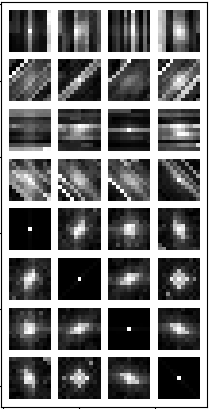
\includegraphics[width=0.35\textwidth]{weights_no_norm}
    \caption[Weights after training without normalisation]{Weight matrix of \emph{S1} after training without weight normalisation.}
    \figlbl{weights_no_norm}
\end{figure}
%
As described in \secref{framework_norm}, the weight is normalised in the range $(0, ..., 1)$.
Normalising the weights is crucial for the proper functioning of the network. Without weight normalisation, lateral support could be dominated by a single cell, resulting in infinite lateral support if trained long enough. In the human brain, there is no such dominance of single cells, and neighbouring cells play an equally important role in providing support \sidecite{kandel_principles_2013}.

After $10$ epochs without weight normalisation, some lateral connections reach a weight above $74$ and dominate the decision process of whether neighbouring cells should remain active.
This leads to undesired activations and weight updates. 
In \figref{weights_no_norm}, the weight matrix after training for $10$ epochs without weight normalisation is depicted.
No clear structure is visible within the weights, and the support provided within the network appears somewhat random. 
Thus, normalisation is not only biologically more plausible but also a necessity to obtain meaningful lateral weights.



\subsection{Initialisation}
In this section, the crucial aspect of weight initialisation is discussed.
In \secref{lateral_init}, it is described that initialising the weight with self-support is essential for the proper functioning of the network.
Two different approaches exist to initialise weights with self-support, as shown in \figref{init_weight_self_support}.
Regardless of the strategy chosen, both approaches lead to identical weight matrices after the training process.
\begin{figure}[h]
    \centering
    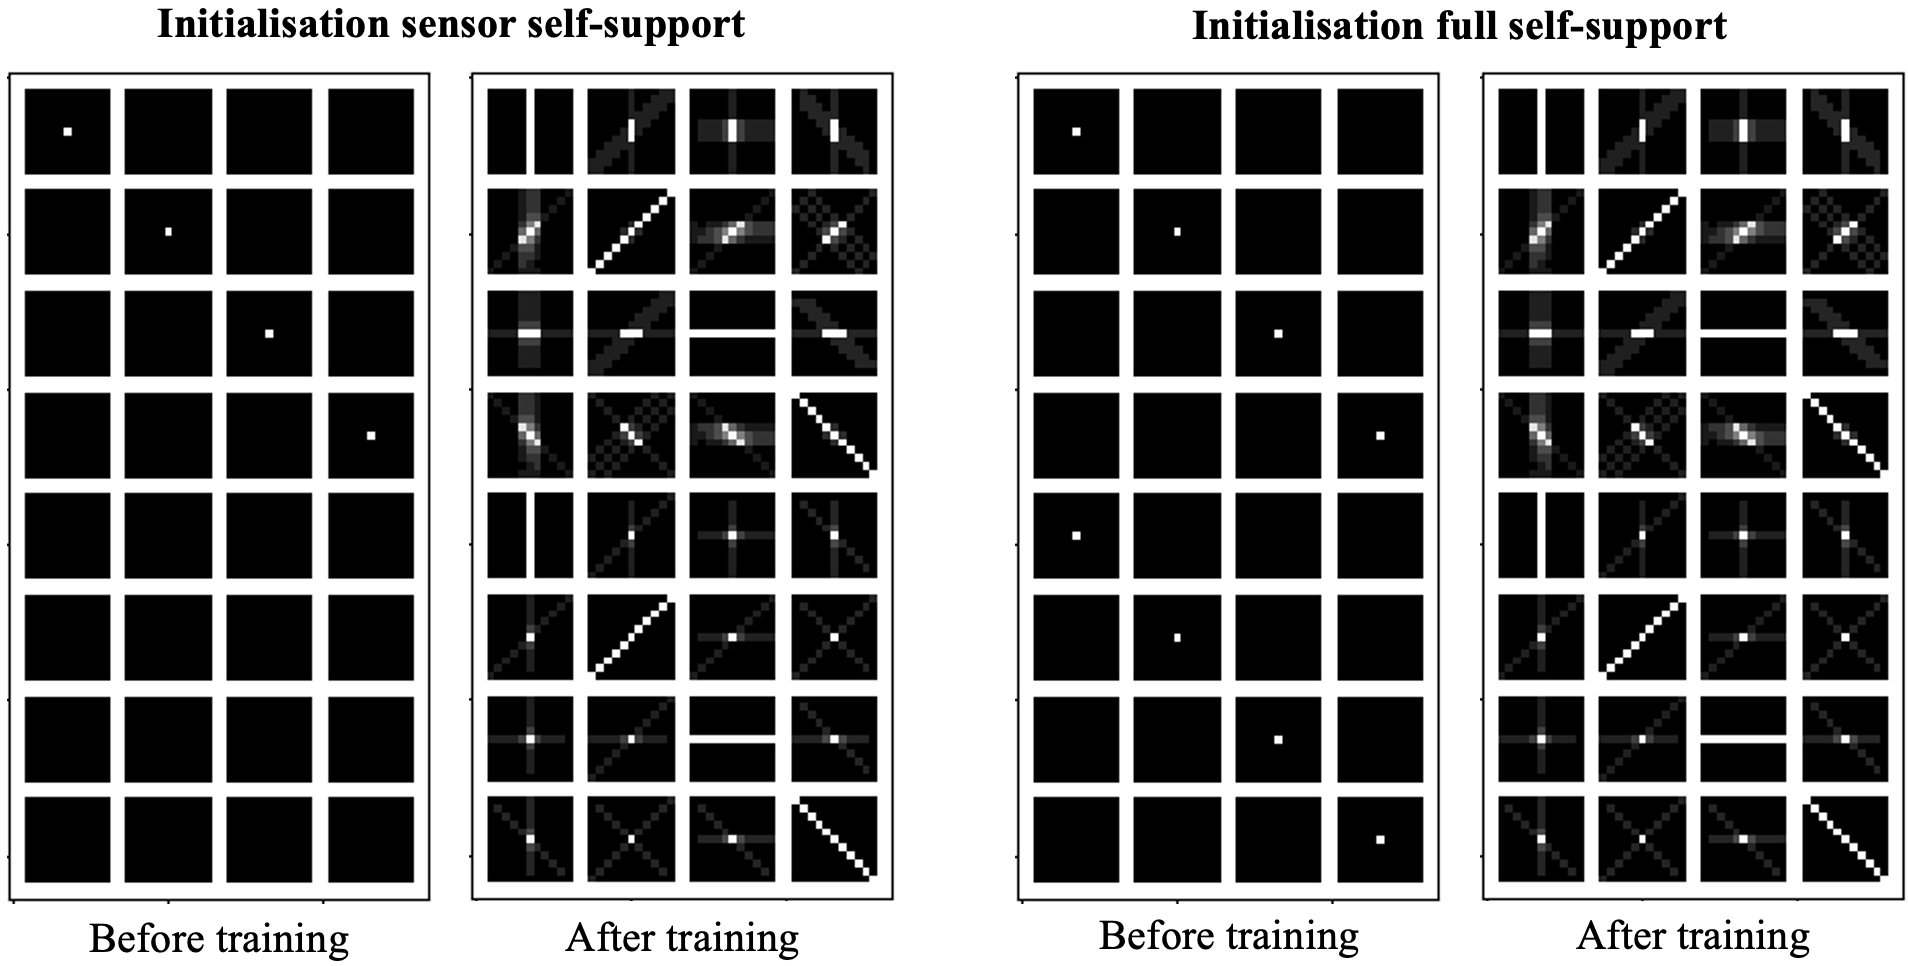
\includegraphics[width=0.99\textwidth]{init_weight_self_support}
    \caption[Weight initialisation with self-support]{Two different ways of initialising the weights of \emph{S1} with self support. For both initialisation strategies, the initial weights are shown on the left and the weights after training on the right.}
    \figlbl{init_weight_self_support}
\end{figure}
\begin{figure}[h]
    \centering
    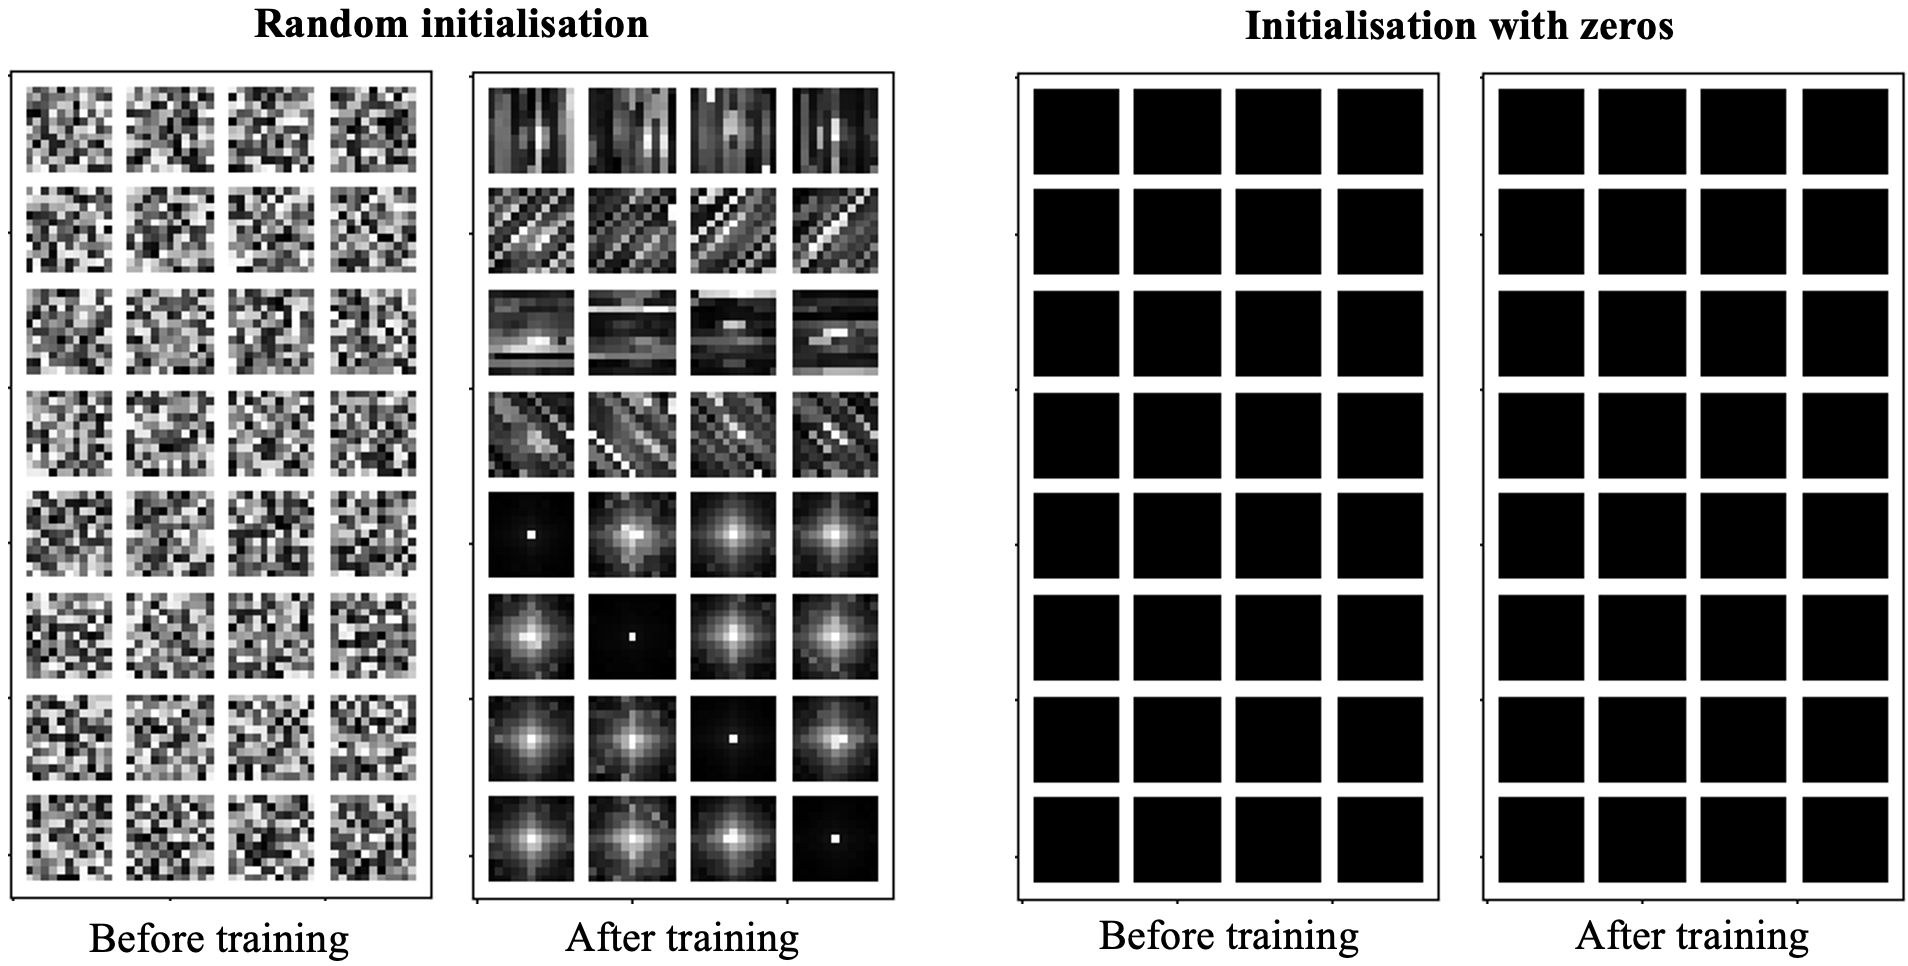
\includegraphics[width=0.99\textwidth]{init_weight_not_working}
    \caption[Random weight initialisation]{Two different ways of initialising the weights of \emph{S1}. The random weight initialisation strategy is shown on the left side of the image, and the zero initialisation strategy is shown on the right side. For both initialisation strategies, the initial weights are shown on the left and the weights after training on the right.}
    \figlbl{init_weight_not_working}
\end{figure}

However, it is important to note that not all weight initialisation strategies lead to good results. 
In \figref{init_weight_not_working}, two other strategies and the resulting weight matrix after training is shown:
Initialising the weights randomly leads to support between cells that should not support each other.
Consequently, this results in unwanted network activations, and the network converges towards weight parameters where the weights are almost identical across all output channels and do not provide lateral support in the desired manner.
If, on the other hand, the weights are initialised with zeros, the network has no active outputs. Consequently, all cells are immediately deactivated, and the weights remain unchanged during Hebbian learning.

In conclusion, using one of the two self-support weight initialisation strategies shown in \figref{init_weight_self_support} is crucial. These methods ensure proper functioning and effective learning, unlike the random or zero weight initialisation strategies depicted in \figref{init_weight_not_working}.

\section{Support Quality}
%
\begin{figure}[h]
    \centering
    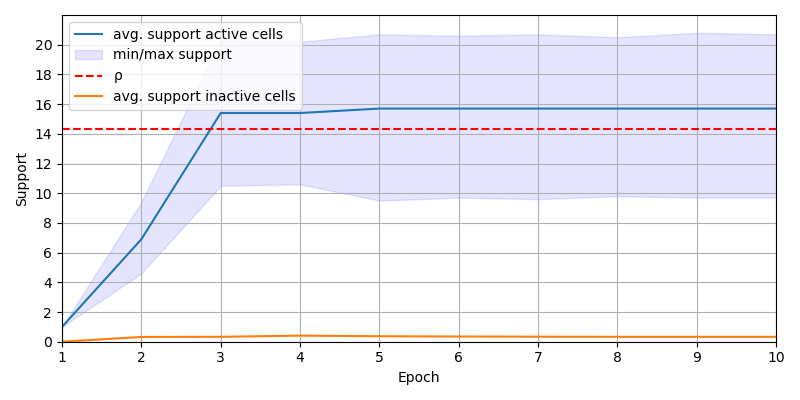
\includegraphics[width=0.99\textwidth]{support_strength}
    \caption[Average lateral support]{The average lateral support received by active and inactive cells during training. The y-axis shows the support, and the x-axis the training epoch. The blue line is the average, and the light blue interval is the min./max. support an active cell receives during training when no inhibition is used; the green interval represents the average/min./max. support an active cell receives support when inhibition is used; the orange line is the average support inactive cells receive. The dotted red line is the inhibition limit $\rho$, marking the threshold where the support is reduced.}
    \figlbl{support_strength}
\end{figure}
%
In \figref{support_strength}, the support strength received by active and inactive cells during training is presented before the activation strength is normalised and translated into an activation probability.
The green interval depicts the support with inhibition and the blue interval without inhibition.

Before training, only self-support exists, i.e. the received support for active cells is $1$.
After training for $3$ epochs, the average support active cells receive increases to $13.8$ with inhibition and $15.7$ without inhibition.
At this point in training, most lateral connections have converged to a synaptic weight strength of $1$.
Thus, on average, a single cell is supported by approximately $14$ neighbouring cells.
On the other hand, inactive cells receive, on average, a lateral support of $0.3$, significantly less than active cells.
Thus, active cells receive much more lateral support after training, while inactive cells still do not receive significant support.
The support difference between active and inactive cells increases from $1$ at the beginning of training to $13.8$ after training.
This increase in support implies that it becomes much more difficult for individual cells to become active and explains why noise can be filtered efficiently.

The support active cells receive is limited by the inhibitory strength $\rho = 1.3\cdot n_l = 14.3$.
When a cell exceeds this threshold $\rho$, its activation probability is linearly reduced.
This effect is visible when comparing the blue interval (without inhibition) with the green interval (with inhibition). With inhibition, the support strength for each cell is pushed below $\rho$, depicted as the red dotted line.

In \figref{support_strength}, it is shown that cells can receive lateral support strengths of up to $21$ when no inhibitory signals are present in the network (see the max. values of the blue interval).
However, such strong support leads to undesired effects, as discussed in the next section.

The results depicted in \figref{support_strength} demonstrate that \emph{S1} builds net fragments as expected. The gap between the support strength of active and inactive cells becomes bigger during training, ensuring that only cells representing known patterns remain active.

\subsection{Inhibition}\seclbl{results_inhibition}
%
\begin{figure}[h]
    \centering
    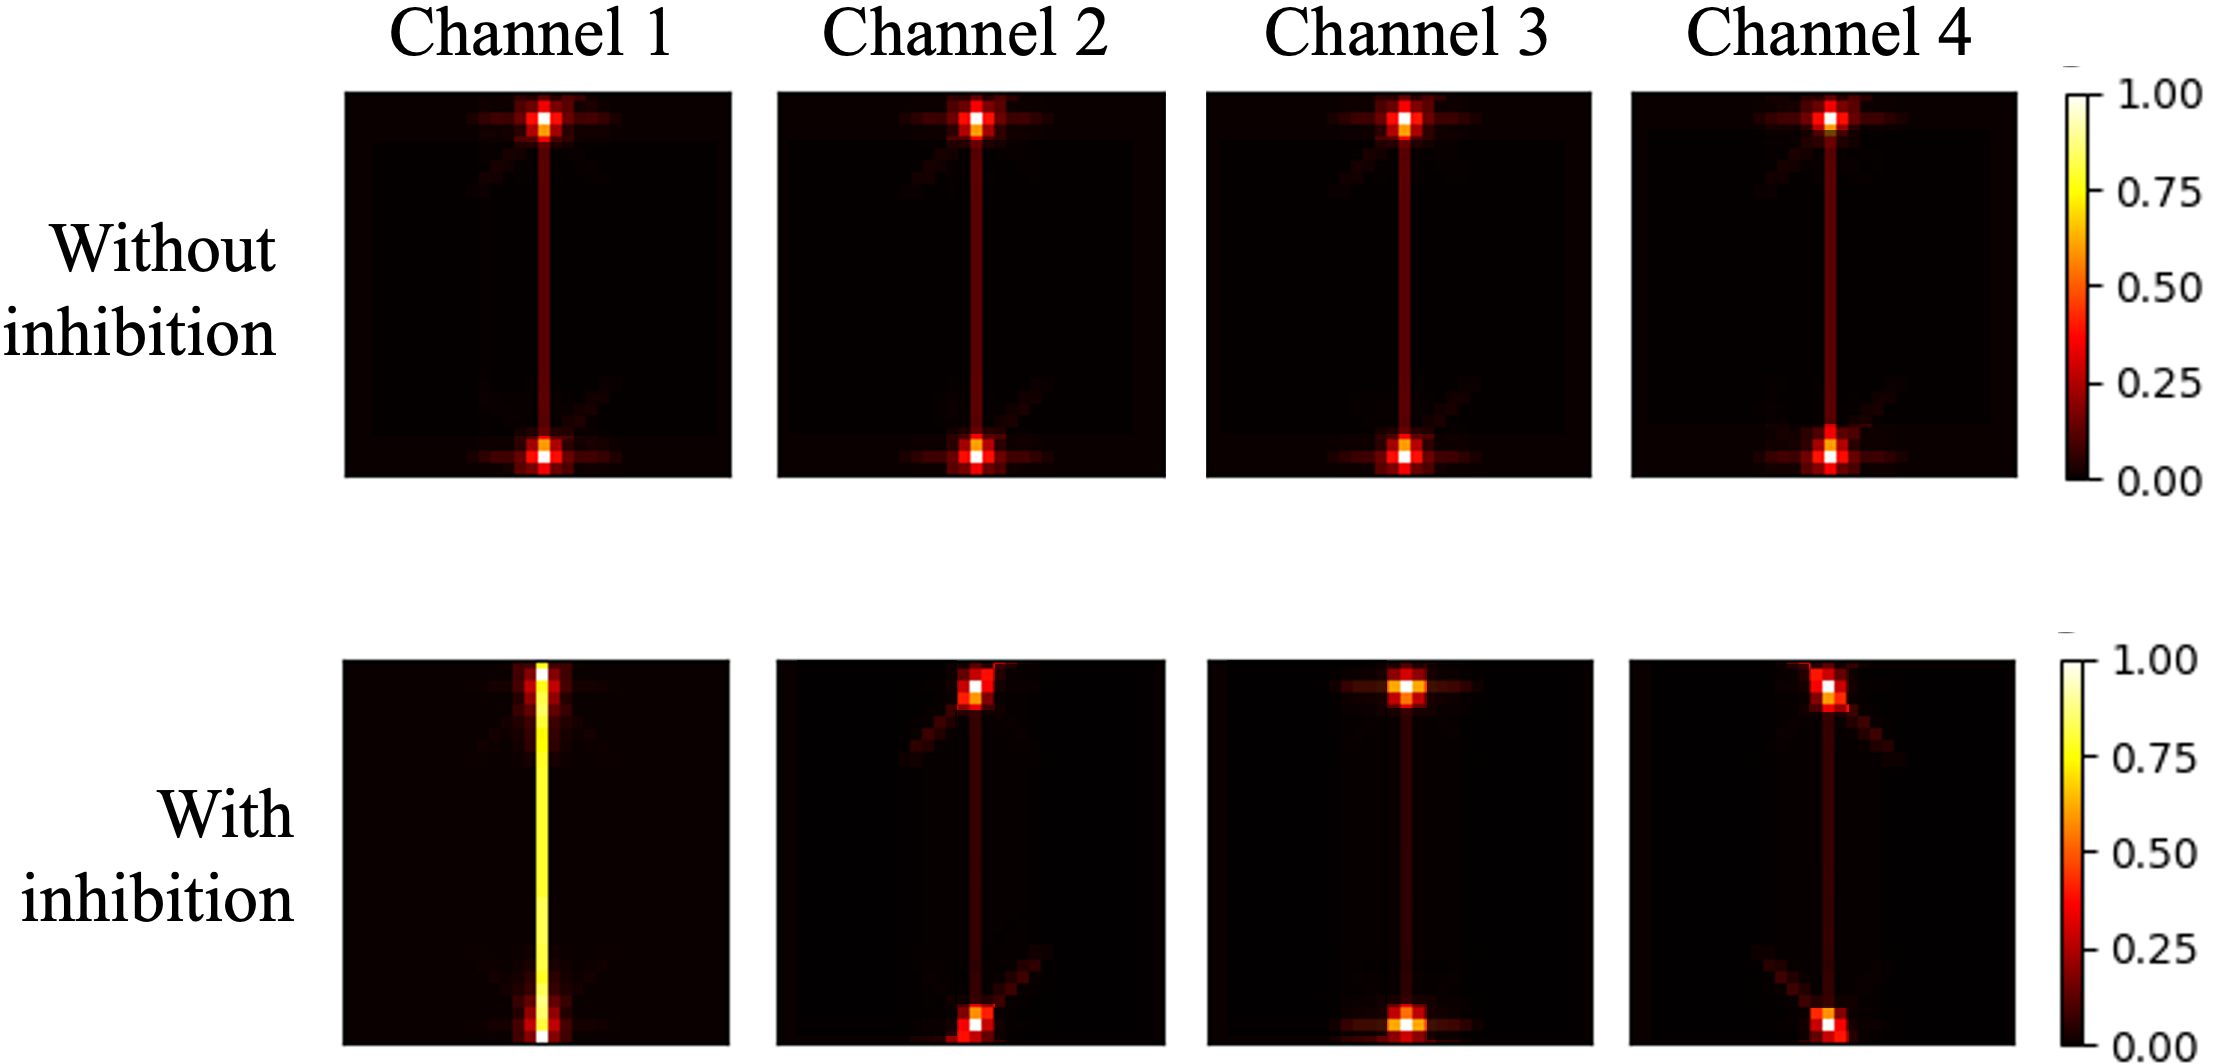
\includegraphics[width=0.79\textwidth]{inhibition_heatmap}
    \caption[Activation heatmap with and without inhibition]{The activation heatmap indicates the activation probability for all cells across the four channels. The upper row shows the probability without inhibition and the lower row with inhibition.}
    \figlbl{inhibition_heatmap}
\end{figure}
%
The following examines the impact of the inhibition threshold $\rho$. The activation heatmap shown in \figref{inhibition_heatmap} displays the activation probabilities for cells across four channels when a vertical line is fed into a model.
The top row shows the probabilities of a model trained without inhibition, while the bottom row shows the probabilities of a model trained with inhibition.

As discussed, all filters are active at the line ends, leading to many active cells and high lateral support in that region.
Specifically, the cell located at the line end receives lateral support from up to $21$ neighbouring cells if no inhibition is used.
When an activation strength of $21$ is mapped to an activation probability of $1.0$ and an activation strength of $0$ to $0.0$, the cells receive activation probabilities as visualised in the upper row of \figref{inhibition_heatmap}.
The pixels at the line ends are dominant and have an activation probability of $1.0$, while the other pixels on the line have an activation probability of approximately $0.4$.
Therefore, only the cells at the line ends have a high activation probability but not the other cells depicting the middle of the line.

Introducing inhibition effectively addresses this issue.
With inhibition, the lateral support is limited to $\rho$.
The effect of inhibition on the activation probability per cell is shown in the second row of \figref{inhibition_heatmap}.
Notably, the activation probabilities of cells at the line ends remain high. However, the activation probabilities of the other pixels depicting the vertical line increase significantly, especially in the first channel, which represents vertical line features.
Thus, inhibition introduces an upper activity threshold so that regions with many active features are limited in providing mutual support.

Please note that the two heatmaps in \figref{inhibition_heatmap} stem from different models.
Inhibition strongly influences the training process, and ``turning on'' inhibition would not convert the activation probabilities in the first into the ones shown in the second row.
Instead, inhibition normalises the activation probabilities throughout the training process, influencing weight updates.
Without inhibition, the activations are dominated by line ends, causing all channels to learn similar features.
With inhibition, the channels specialise more on distinct features as no feature dominates the learning process. Therefore, the weights (and thus the activation probabilities shown on the second row of \figref{inhibition_heatmap}) are more diverse.

\section{Conclusion}
The previous sections discuss the obtained results, thereby focusing on specific aspects.
In conclusion, \emph{S1} can build net fragments \sidecite{von_der_malsburg_theory_2022, von_der_malsburg_concerning_2018}, and it is demonstrated that these fragments associate input patterns with learned patterns, thereby removing noise or reconstructing occluded parts of objects.
Thus, the experiments demonstrate that net fragments can be implemented according to the proposed principles.
Since removing noise and reconstructing objects improves representations over multiple timesteps, it is considered a hierarchical processing of features without being subject to early commitment \sidecite{marr_vision_2010}.

This is considered an essential step towards implementing the proposed framework.
Implementing projection fibres \sidecite{tanigawa_organization_2005, greig_molecular_2013} is based on the principle of comparing local features in \emph{S1} and \emph{S2} and initiating a mapping between them if neighbouring fibres agree \sidecite{bienenstock_neural_1987, lades_distortion_1993, wiskott_face_1996}.
Such a mapping only works well if patterns in the two stages are highly similar.
As demonstrated in this chapter, this can be achieved with net fragments that either turn off cells representing unknown patterns that are not present in \emph{S2} and thus cannot be mapped or support and reconstruct (i.e. optimise) existing patterns to become more similar to patterns stored in \emph{S2}.
Thus, the conducted experiments lay the foundation for future research and implementing projection fibres.


\setchapterpreamble[u]{\margintoc}
\chapter{Future Work}\chlbl{future_work}
\section{Discussion}
Deep learning networks have demonstrated their exceptional capabilities as feature extractors. 
Recent advancements in scaling have brought them to a level where they hold the potential for widespread applicability across various tasks in our everyday lives.
Nevertheless, they have intrinsic limitations, and the prospect of overcoming these barriers remains uncertain.
This thesis presents a vision framework that addresses several of these challenges, primarily focusing on mitigating early commitment and facilitating object-agnostic transformation invariance.

The proposed framework is strongly inspired by the biological brain, the only known system to which we attribute true intelligence.
One of this thesis's main contributions is identifying neuroscientific findings and their subsequent integration within the contours of a computational framework.

A key difference between the proposed system and deep networks is that deep learning lies in the mechanism of building consistency:
Deep networks optimise consistency at a single point in the network by comparing its prediction with a teaching signal.
A global error correction algorithm such as backpropagation adjusts all components in the network to minimise inconsistencies at a single point.

In contrast, the proposed framework implements a model that optimises consistency at every point in the network, akin to the human brain.
It encompasses three building blocks, all using binary Bernoulli neurons.
These biologically plausible neurons allow net fragments to be implemented and improve robustness. However, their full optimisation within the prevailing computational framework remains an ongoing endeavour.

The sensory stage \emph{S0} corresponds in the biological context to the eyes and extracts features from images.
The implementation could involve the first convolutional layer of a pre-trained autoencoder. Given the well-established feature extraction capabilities of CNNs, it is reasonable to expect the suitability of this layer without having done extensive experiments within this thesis.

The feature building stage \emph{S1}, inspired by the primary visual cortex, leverages lateral connections to form net fragments, groups of neurons that support each other's activity.
This stage is well examined in this thesis and iteratively refined based on empirical investigations.
The experiments confirm the usefulness of lateral connections in tasks such as occluded object reconstruction and noise reduction.

The prototype stage \emph{S2} takes inspiration from the ventral visual stream and the temporal cortex.
It uses projection fibres to map network fragments onto object prototypes. While this aspect is well explained theoretically in this thesis, it lags behind \emph{S1} in empirical validation and refinement.


At its core, the entire network is based on the principles of self-organisation, locality and cell consistency.
Network fragments arise from cells communicating with their spatial neighbours, while projection fibres connect neighbouring cells in \emph{S1} and \emph{S2} and seek consistency with neighbouring fibres.
These basic principles are fundamentally different from existing deep networks. In addition, the network incorporates constraints aimed at reducing early commitment and increasing robustness. The iterative process of assembling net fragments and mapping them to object prototypes leads to transformation-invariant feature processing independent of specific objects.

In summary, the proposed framework introduces several promising principles. However, as elaborated in the next section, these principles must be explored and refined further in future work.
Comparing the proposed framework with deep networks is not possible at its current stage as it is far from being developed enough. 
I speculate that deep networks excel at well-defined tasks that can be measured with corresponding metrics because they optimise all network neurons to maximise consistency between a prediction and a task-specific teaching signal at a single network node. Conversely, optimising the consistency at every single point in the network, as done in the proposed framework, might be a way towards more intelligent systems. Such a configuration could harmonise different signals, each contributing to coherent representations in the decision-making processes. By doing so, each signal and cell would cast its vote for a particular course of action and seek consensus without an external source providing a global teaching signal.


\section{Future Work}
This work is a preliminary study for a possible dissertation, focusing on refining the proposed framework.
Consequently, numerous avenues exist for future work to improve the proposed framework. The following section outlines some of the most pressing issues and proposes the next steps.


\subsection{Alternative Cells in \emph{S1}}\seclbl{future_alt_cells}
In the context of \emph{S1}, individual cells represent distinct features that are localised in a specific spatial location. These cells support each other's neuronal activity. As outlined in \secref{framework_neuroscience}, these cells can contribute to mutually exclusive net fragments. For example, cell $A$ may participate in a fragment with cell $B$ and another fragment with cell $C$, while cell $B$ and $C$ avoid simultaneous activation. This exceeds the functional capacity of cell $A$, and a copy of $A$ is needed to establish separate lateral connections with cell $B$ and $C$.

The \secref{framework_alt_cells} described that alternative cells could be implemented by duplicating the output channels of the weight matrix $\boldsymbol{W}$ of \emph{S1}.
Alternative cells contribute to different net fragments and are mutually exclusive.
Consequently, competition between these alternative cells is required to ensure that only a winning cell can become active and that activity in alternative cells is suppressed\sidenote{Activity can be suppressed by inhibition, as it is already implemented in \emph{S1}.}.

Preliminary experiments suggest that the initially similar characteristics between alternative cells make it difficult to establish effective competition and that this initial symmetry that needs to be broken first.
Introducing controlled randomness during the initial phase could increase the stochasticity of the learning process. This randomness can potentially enhance differentiation and separation between these different cells.

Furthermore, an extension of Hebbian learning is needed to enable the forgetting of previously learned patterns.
Currently, each update only increases the weights, which strengthens lateral support.
However, some updates could inadvertently create incorrect connections between different (alternative) cells.
The following section describes negative Hebbian learning, a mechanism that allows forgetting learned connections and seems crucial to implementing alternative cells.
This mechanism eliminates the need to carefully prevent false updates during the initial training phase, as erroneous updates can be corrected as soon as the alternative cells are separated enough.

\subsection{Negative Hebbian Learning within \emph{S1}}
The previous section describes how negative Hebbian learning can help to realise alternative cells.
While conventional Hebbian learning increases the synaptic weights between simultaneously active neurons, negative Hebbian learning introduces a complementary process by decreasing the synaptic weight between cells that fire disjoint.
These negative updates are not only crucial in the formation of alternative cells but also in gradually eliminating less significant patterns that have been imprinted during the training phase.

Implementing negative Hebbian updates is challenging, especially when the data is dominated by negative correlations\sidenote{The dataset contains more samples where two feature cells are active separately than simultaneously.}, as shown in \chref{neg_hebb_updates}.
One possible strategy to overcome this problem is using a significantly lower learning rate for negative updates than for positive ones.
This asymmetry ensures that the process of forgetting is slower than the process of learning, preventing the abrupt erasure of acquired patterns.
Another solution is alternative cells: If two patterns have a positive correlation at one point and a negative correlation at another point (as in the example shown in \chref{neg_hebb_updates}), these patterns can be processed differently by employing alternative cells, effectively maintaining their distinct representations.


\subsection{Refine \emph{S2}}
An important task for future work is the empirical improvement of \emph{S2}, which has only been theoretically developed based on identified neuroscientific findings. The current blueprint describing its implementation has to be further refined by conducting experiments.

In the first phase, the integration and evaluation of projection fibres based on shifter circuits \sidecite{anderson_shifter_1987, olshausen_neurobiological_1993} should be done and explored within the proposed framework.
During this process, also different object views should be explored (provided by the medium processing loop). Currently, these views are only used during evaluation, but once \emph{S2} is implemented, they can be crucial in learning to associate different views to the same prototype, encouraging transformation-invariant mappings.

Once an initial effective mapping has been created, the presumed simplifications can be avoided (c.f. \secref{framework_s2}). In particular, novel prototypes from unseen objects can be stored automatically, the prototypes can be iteratively improved throughout training, projection fibres can be learned dynamically, and the network can be extended to interpret complete scenes, thus going beyond the limits of object-centric images.






\subsection{Scaling to Different Datasets}
In the experiments, a dataset comprising straight lines is used, effectively illustrating the principles and enhancing understanding of the proposed framework.
Nevertheless, assessing the models' scalability to larger and more diverse datasets is important.
One possible avenue is to use traditional classification datasets such as MNIST \sidecite{lecun_gradient-based_1998}, CIFAR-10 \sidecite{krizhevsky_learning_2009}, or ImageNet \sidecite{russakovsky_imagenet_2015}.
However, it is important to note that the primary goal is not to push benchmarks for image classification.
Rather, the goal is to obtain high-quality object representations.

This endeavour may require building new datasets generated by an image rendering engine capable of simulating 3D objects and generating data in real-time.
Using such an engine allows to generate visualisation of objects undergoing realistic-looking transformations and depth rotations.
This method allows the evaluation of the model's ability to process complex and diverse visual data that more closely resembles real-world scenarios.
Moreover, these transformations are an integral part of the proposed processing loop and even allow interaction with objects. For example, the model could determine the optimal viewing angle when looking at an object and thus improve its representation to ensure internal consistency.




\subsection{Multi-Modality}\seclbl{framework_multi_modality}
This work focuses on a framework for computer vision. However, the architecture has broader applicability and can be used for processing different sensor signals and be used in multimodal settings \cite{ngiam_multimodal_2011, liu_learn_2018, baltrusaitis_multimodal_2019}.
Having similar cell architectures processing different kinds of signals is also in line with findings from neuroscience \sidecite{mountcastle_organizing_1978, mountcastle_columnar_1997}.

In the case of images, net fragments in \emph{S1} represent learned visual patterns that are part of an object's surface and are mapped with protection fibres to object prototypes that describe the visual appearance of objects. 
The same architectural structure can be applied to other types of signals. For example, an alternative sensory system could perceive audio signals. In this scenario, the local support in \emph{S1} would extend over nearby frequency ranges and time intervals. Consequently, phonemes or syllables could correspond to frequently occurring patterns that are captured and supported by net fragments. In the second stage (\emph{S2}), a sequence of phonemes or syllables could be mapped onto word prototypes.

Different sensory systems could even have separate domain-specific \emph{S1} stages in a multimodal setting, while the prototypes in \emph{S2} could be shared across modalities. This arrangement would allow the integration of various sensor signals and facilitates the creation of internal object representations with multiple modalities.

%%%%%%%%%%%%%%%%%%%%%%%%%%%%%%%%%%%%%%%%%%%%%%%%%%%%%%%%%%%%%%%%%%%%%%%%%%%%%%%%
\appendix

% Transition page
\pagelayout{wide}
\addpart{Appendix}
\pagelayout{margin}

\renewcommand\home{./}
\chapter{Results: Online Sources}\chlbl{online_sources}
%
\begin{figure}[h]
    \centering
    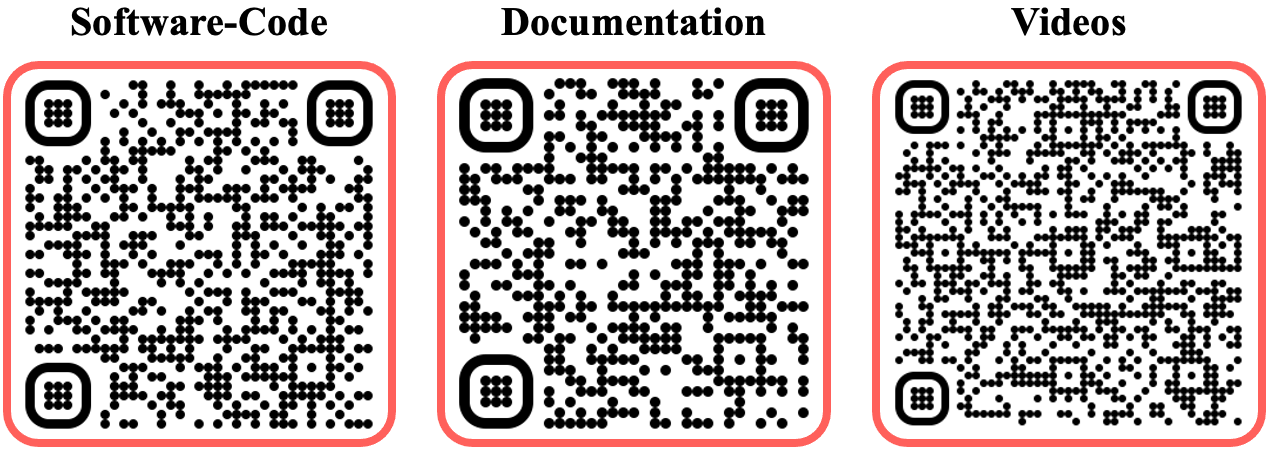
\includegraphics[width=0.79\textwidth]{qr_links}
    \caption[QR-Codes with links to sources]{QR-Codes with links to sources. The first code directs to the GitHub repository containing the source code, the second code to the repository containing the \LaTeX files to build this documentation, and the third code points to video visualisations of the results.}
    \figlbl{qr_links}
\end{figure}
%
The codebase and results from this thesis have been released as open source on GitHub: The code is available at \href{https://github.com/sagerpascal/lateral-connections}{github.com/sagerpascal/lateral-connections}, and the documentation is available at \href{https://github.com/sagerpascal/msc-thesis}{github.com/sagerpascal\\/msc-thesis}.
Furthermore, a GitHub webpage provides video visualisations from some of the results is available at \href{https://sagerpascal.github.io/lateral-connections/results/final_results.html}{sagerpascal.github.io/lateral-connections/results/final\_results}.
QR codes linking to these URLs are provided in \figref{qr_links} for convenient access using electronic devices.


\section{Video}\seclbl{result_video}
%
\begin{figure}[h]
    \centering
    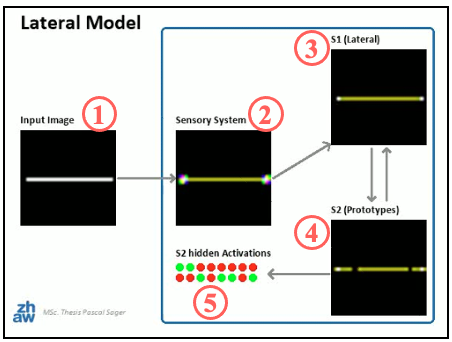
\includegraphics[width=0.99\textwidth]{video_overview}
    \caption[Overview of components visualised in the videos]{An overview of the components visualised in the videos.}
    \figlbl{video_overview}
\end{figure}
%
In the following, the video visualisations accessible at \href{https://sagerpascal.github.io/lateral-connections/results/final_results.html}{sagerpascal.github.io\\/lateral-connections/results/final\_results} are explained.
These explanations are limited to an overview of which components are shown in each video.
An interpretation of the video contents is provided in the corresponding result section.

Two video versions are shown for each experiment, both produced by the same model using the same parameter weights.
In the first video version, the Bernoulli neuron is replaced by a neuron using a fixed threshold.
This provides a video output that is more stable and has no flickering activations caused by sampling from a probability distribution.
For the \emph{S0} and \emph{S1} stages, a threshold of $0.5$ is used. Consequently, neurons with a probability of $\geq 0.5$ are set to $1$, while the other neurons are set to $0$.
A threshold of $0.9$ is used for the \emph{S2} stage, visualising only activities with high certainty that roughly correspond to those accepted by \emph{S1} as feedback signals.
The second video shows the network activities when the Bernoulli neurons are used.

Each video visualises the processing of the input over time.
The first six video frames show how the video is processed over the $T=6$ timesteps of the fast loop, followed by five additional frames depicting the final prediction after the fast loop.
By doing so, viewers have time to analyse the network's activations during this short interruption before the next input is fed into the model, and the process repeats.

\figref{video_overview} shows a single video frame, providing an overview of the components displayed in each video:
\begin{enumerate}
    \item The left part of the video displays the input image fed into the sensory system. It is a binary image with one colour channel, whereby active pixels are depicted in white and inactive pixels are depicted in black.
    \item The activations of the sensory system \emph{S0} are shown in the middle of the video. The sensory system extracts $4$ features at each location. Each feature combination is visualised in a different colour, and areas without activations are depicted in black.
    \item \emph{S1} is visualised in the top right corner. It uses the same colours as the sensory system. However, the activations might differ since neurons with insufficient lateral support are turned off, or other neurons might switch on.
    \item \emph{S2} is shown in the bottom right corner. It uses the same colours as the sensory system and \emph{L1}. The visualisation depicts the returned prototype, i.e., the feedback provided to \emph{S1} after mapping \emph{S1}' activities to the latent variables.
    \item The latent variables of \emph{S2} are shown at the center bottom of the video as $16$ circles. Each circle represents a cell, with green indicating an active cell and red indicating an inactive one. 
\end{enumerate}

For a detailed explanation of the content and observations in each video, please refer to the results chapter of this thesis.

\chapter{Negative Hebbian Learning}\chlbl{neg_hebb_updates}
%
\begin{figure}[h]
    \centering
    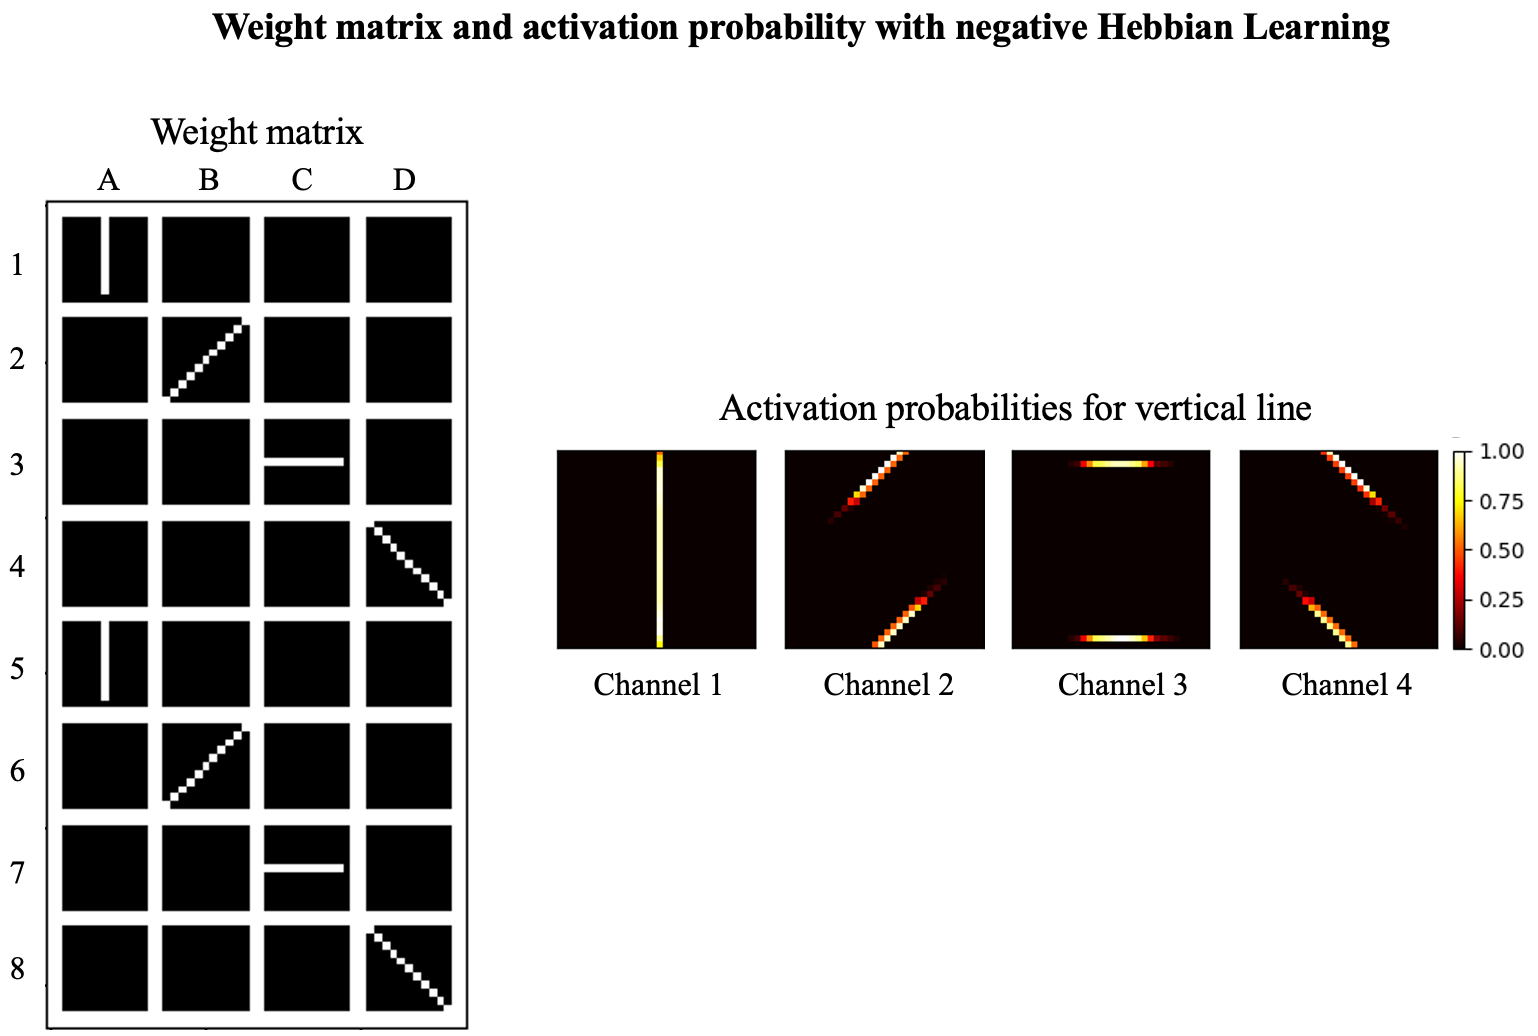
\includegraphics[width=0.99\textwidth]{neg_hebb_learning}
    \caption[Weight matrix and activations with negative Hebbian learning]{The weight matrix and the corresponding activation probabilities for a vertical line of a model trained with negative Hebbian learning.}
    \figlbl{neg_hebb_learning}
\end{figure}
%
This section examines the concept of negative Hebbian Learning in \emph{S1}, a learning paradigm designed to allow neural networks to forget unimportant or inconsistent features. 
In the conducted experiments, only positive Hebbian learning \sidecite{hebb_organization_1949} is used to strengthen connections between active cells.
Conversely, negative Hebbian learning additionally reduces the connection strength between cells that fire disjointly\sidenote{I.e. one cell is active while the other is inactive.}.
While negative Hebbian learning facilitates eliminating previously learned but inconsistent connections, it also poses challenges in maintaining desired lateral connections that are needed to provide support between feature cells.


\figref{neg_hebb_learning} visualises the weight matrix of a model trained with negative Hebbian updates and the activation probabilities if a vertical line fed is into the model.
Despite the divergence of the activation probabilities compared to those of positive Hebbian learning (c.f. \figref{S1_weight_analysis}), these activations are still considered valid representations of lines.
However, the major issue is that the output channels do not rely on multiple distinct features.

For instance, the output channel $A$ representing vertical lines only considers the input channels $1$ and $5$, whereby channel $1$ contains the ``vertical lines features'' from the sensory system, and channel $5$ is its own recurrent connection.
Regrettably, input channels $2$-$4$, which contain additional sensory signals, are disregarded by output channel $A$. Therefore, only cells representing vertical line features support this output channel.
In contrast, positive Hebbian learning considers all input channels, resulting in different features supporting each other.

Consequently, negative Hebbian learning leads to lower lateral support within the network.
This might not be an issue for the used line dataset but is crucial for real-world scenarios\sidenote{For example, one channel could represent eyes and another channel eyelashes. These features should support each other.}.
Negative Hebbian learning, while facilitating the filtering out of irrelevant features, also tends to make features mutually exclusive, which prevents learning adequate support between them.

\begin{figure}[h]
    \centering
    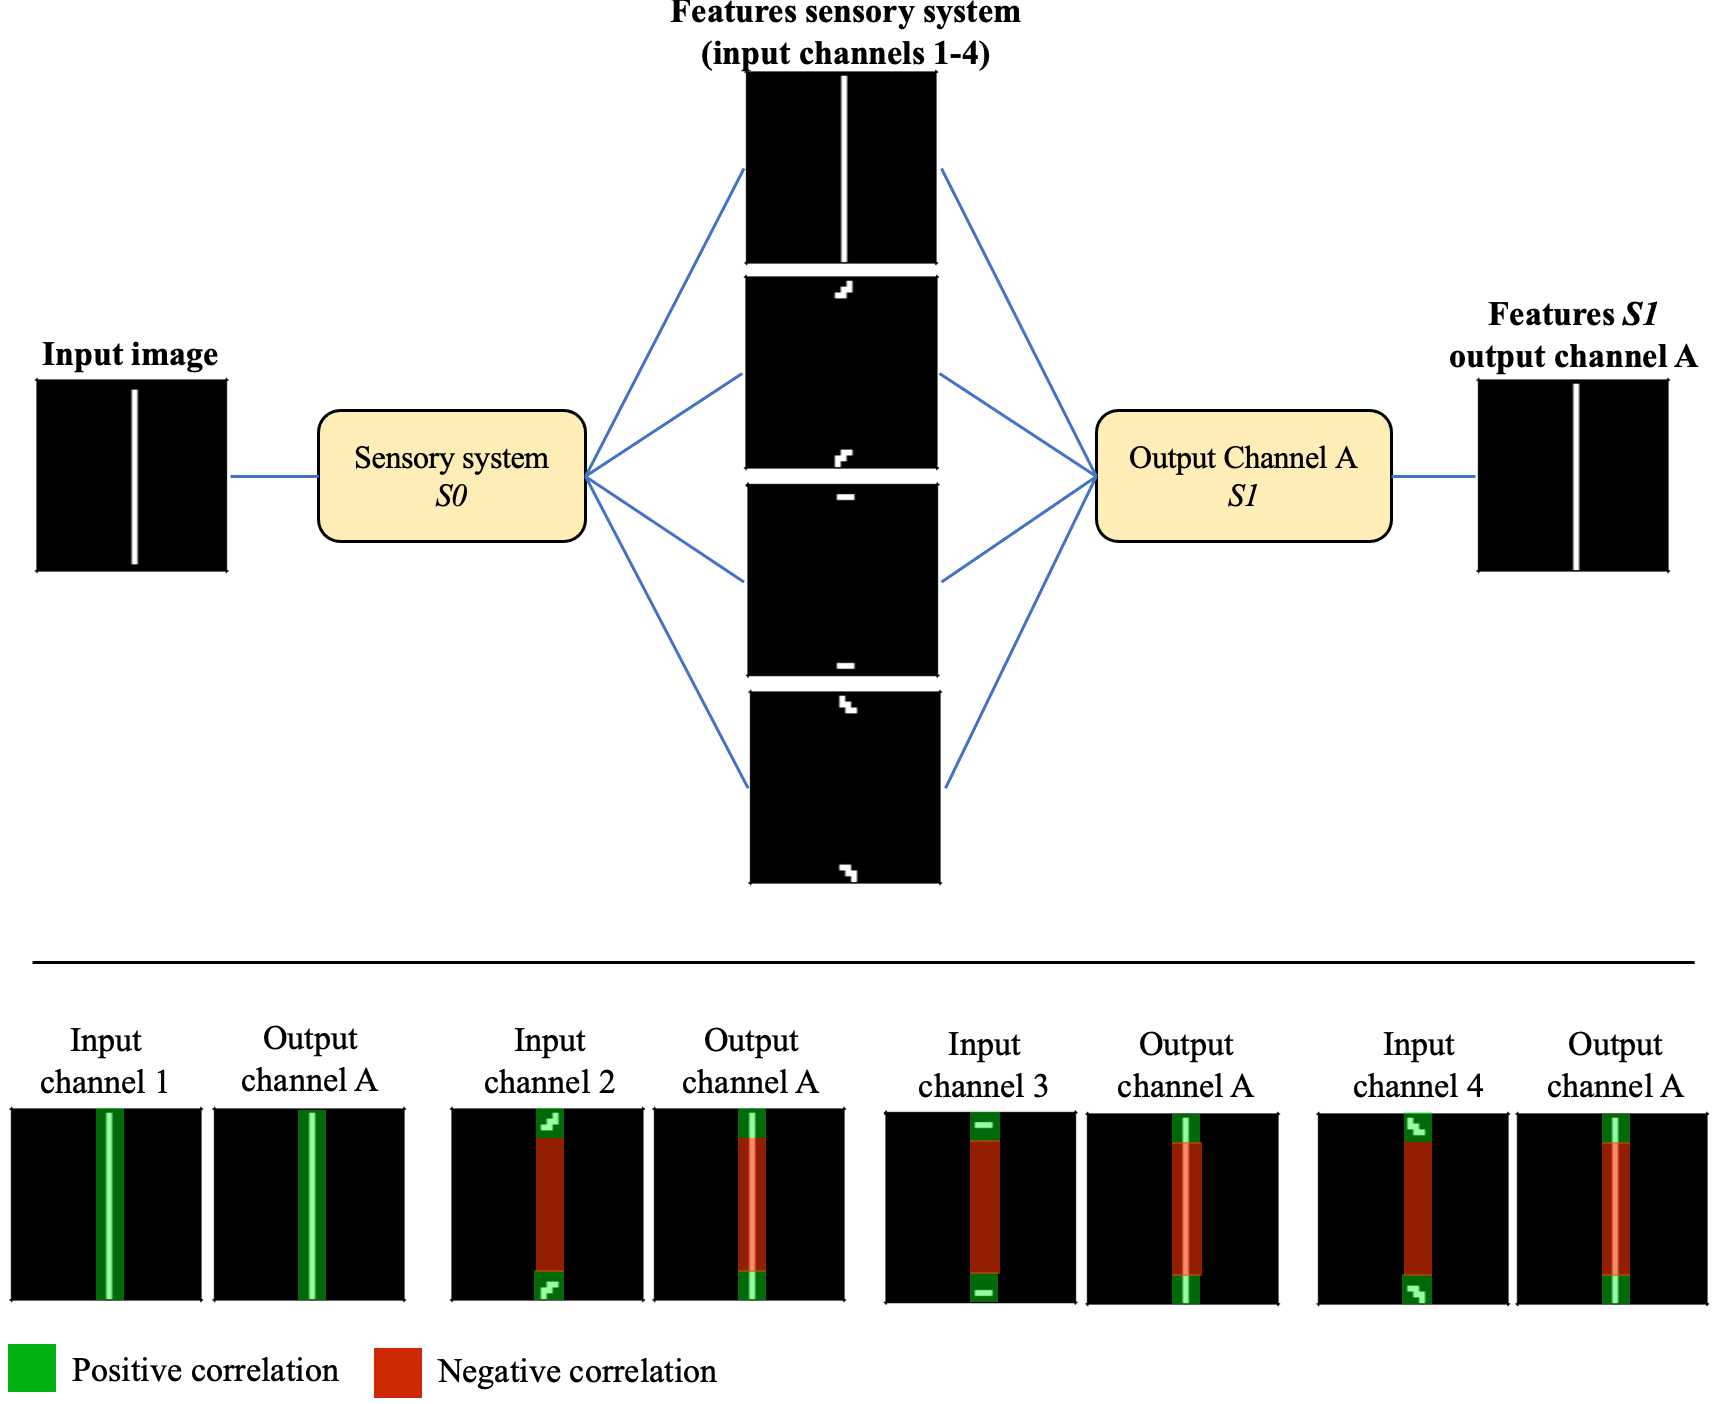
\includegraphics[width=0.99\textwidth]{correlations_hebb_learning}
    \caption[Feature correlation analysis]{Correlation between features from sensory input channels and the output channel $A$. The upper part of the images visualises the sensory features fed into output channel $A$ and the expected result. The lower part of the image indicates where positive and negative correlation occurs between sensory channels and output channel $A$.}
    \figlbl{correlations_hebb_learning}
\end{figure}
%
The primary issue is that, except for one input channel, there are more negative correlations between the input channels and a single output channel, as illustrated in \figref{correlations_hebb_learning}.
In this context, ``negative correlation'' refers to disjointly active cells, while ``positive correlation'' refers to cells that fire together.
In the case of the vertical line, the output channel $A$ is expected to reassemble the line roughly.

Hebbian learning compares this output with the input channels, strengthening the weights for positively correlated input-output pairs and weakening them for negatively correlated pairs.
These correlations are visualised in the lower part of \figref{correlations_hebb_learning}.
Input channel $1$ and output channel $A$ have high similarity. Therefore, the activations between input and output have a positive correlation, and the corresponding lateral connections undergo a positive Hebbian update.
However, all the other channels have a positive correlation only at the line ends and a negative correlation in the middle section of the line.
Consequently, there is more negative than positive correlation, and these features undergo more negative than positive updates.
This causes the lateral support learned at the line ends to be suppressed by the negative updates triggered by the negative correlation in the middle of the line.

The resolution to this issue remains unclear and requires additional experiments. One potential approach is to use a significantly lower learning rate for negative updates than for positive updates; another solution could be to introduce alternative cells (c.f. \secref{future_alt_cells})




%%%%%%%%%%%%%%%%%%%%%%%%%%%%%%%%%%%%%%%%%%%%%%%%%%%%%%%%%%%%%%%%%%%%%%%%%%%%%%%%
%%%%%%%%%%%%%%%%%%%%%%%%%%%%%%%%%%%%%%%%%%%%%%%%%%%%%%%%%%%%%%%%%%%%%%%%%%%%%%%%
\backmatter
\setchapterstyle{plain}


%%%%%%%%%%%%%%%%%%%%%%%%%%%%%%%%%%%%%%%%%%%%%%%%%%%%%%%%%%%%%%%%%%%%%%%%%%%%%%%%
\defbibnote{bibnote}{Here is the list of references in citation order.\par\bigskip}
\printbibliography[heading=bibintoc, title=Bibliography, prenote=bibnote]


%%%%%%%%%%%%%%%%%%%%%%%%%%%%%%%%%%%%%%%%%%%%%%%%%%%%%%%%%%%%%%%%%%%%%%%%%%%%%%%%
\printindex


%%%%%%%%%%%%%%%%%%%%%%%%%%%%%%%%%%%%%%%%%%%%%%%%%%%%%%%%%%%%%%%%%%%%%%%%%%%%%%%%
%\clearpage
%\thispagestyle{empty}
%\null%
%\clearpage
%\includepdf{cover-back.pdf}

%%%%%%%%%%%%%%%%%%%%%%%%%%%%%%%%%%%%%%%%%%%%%%%%%%%%%%%%%%%%%%%%%%%%%%%%%%%%%%%%
\end{document}
%%%%%%%%%%%%%%%%%%%%%%%%%%%%%%%%%%%%%%%%%%%%%%%%%%%%%%%%%%%%%%%%%%%%%%%%%%%%%%%%
